\documentclass[10pt]{article}
\usepackage{style/fullpage}
\usepackage{style/underscore}
\usepackage{style/environ}
\usepackage{color}
\usepackage{alltt}
\usepackage{graphicx}
\usepackage{etoolbox} % for @for \do ??
\usepackage[hidelinks]{hyperref} % for hyperref
\usepackage{xstring}
\usepackage{adjustbox}

%\IfFileExists{minted.sty}{
%\usepackage{minted}
%\newminted[ccode]{c}{}
%\newminted[cxxcode]{c++}{}
%\newminted[fcode]{fortran}{}
%\newminted[pycode]{python}{}
%\newmint[cfuncsig]{c}{}
%\newmint[cxxfuncsig]{c++}{}
%\newmint[ffuncsig]{fortran}{}
%\newmint[pyfuncsig]{python}{}
%}{
\usepackage{listings}
\lstnewenvironment{ccode}
    {\lstset{language=C, breaklines=true, breakautoindent=true}}
    {}
\lstnewenvironment{cxxcode}
    {\lstset{language=C++, breaklines=true, breakautoindent=true}}
    {}
\lstnewenvironment{fcode}
    {\lstset{language=Fortran, breaklines=true, breakautoindent=true}}
    {}
\lstnewenvironment{pycode}
    {\lstset{language=Python, breaklines=true, breakautoindent=true}}
    {}
%}

\newcommand{\apih}[2]{
\noindent
\section*{#1}
\label{api:#1}
\textit{#2}
}

%\newcommand{\optype}[1]{
%\newline
%\textbf{Operation Type:}#1
%\newline
%}

\newcommand{\wcoll}{
\noindent
\textcolor{blue}{Operation Type:} Collective on the world processor group
\newline
}
\newcommand{\dcoll}{
\noindent
\textcolor{blue}{Operation Type:} Collective on the default processor group
\newline
}
\newcommand{\gcoll}{
\noindent
\textcolor{blue}{Operation Type:} Collective on the processor group inferred from the arguments
\newline
}
\newcommand{\ncoll}{
\noindent
\textcolor{blue}{Operation Type:} One-sided (non-collective)
\newline
}
\newcommand{\local}{
\noindent
\textcolor{blue}{Operation Type:} Local
\newline
}

\newenvironment{desc}{
\noindent
\textcolor{blue}{API description:}\par}{}

\newenvironment{cdesc}{
\noindent
\textcolor{blue}{C API description:}\par}{}

\newenvironment{fdesc}{
\noindent
\textcolor{blue}{Fortran API description:}\par}{}

\newenvironment{cxxdesc}{
\noindent
\textcolor{blue}{C++ API description:}\par}{}

\newenvironment{fapi}{
\noindent
\textcolor{blue}{Fortran Interface}
\small
}{
}

\newenvironment{f2dapi}{
\noindent
\textcolor{blue}{Fortran 2D Interface}
\small
}{
}

\newenvironment{pydesc}{
\noindent
\textcolor{blue}{Python API description:}

}{}

\newenvironment{capi}{
\noindent
\textcolor{blue}{C Interface}
\small
}{
}

\newenvironment{cxxapi}{
\noindent
\textcolor{blue}{C++ Interface}
\small
}{
}

\newenvironment{pyapi}{
\noindent
\textcolor{blue}{Python Interface}
\small
}{
}

\newenvironment{funcargs}{\noindent\begin{tabular}{@{}p{0.16\textwidth}@{}p{0.14\textwidth}@{}p{0.58\textwidth}@{}p{0.08\textwidth}@{}}}{\end{tabular}}

\newcommand{\funcarg}[4]{\texttt{#1}&\texttt{#2}&\texttt{#3}&\texttt{#4}\\}

\newcommand{\inarg}[3]{\texttt{#1}&\texttt{#2}&\texttt{#3}&\textcolor{blue}{\texttt{input}}\\}

\newcommand{\inoutarg}[3]{\texttt{#1}&\texttt{#2}&\texttt{#3}&\texttt{\textcolor{blue}{in}/\textcolor{red}{out}}\\}

\newcommand{\outarg}[3]{\texttt{#1}&\texttt{#2}&\texttt{#3}&\textcolor{red}{\texttt{output}}\\}

\definecolor{copper}{RGB}{213,117,0}
\definecolor{silver}{RGB}{112,114,118}
\definecolor{bronze}{RGB}{168,60,15}
\definecolor{gold}{RGB}{241,171,0}
\definecolor{onyx}{RGB}{36,36,36}
\definecolor{platinum}{RGB}{178,179,181}

\newcounter{SeeAlsoCounter}
\makeatletter
\newcommand*{\seealso}[1]{%
\noindent
\textcolor{blue}{See Also:}
\newline
\def\mystring{#1}
\StrCount{\mystring}{,}[\commacount]
\setcounter{SeeAlsoCounter}{0}
\@for\arg:=#1\do{%
  \hyperref[api:\arg]{\nameref*{api:\arg}}\ifnum\value{SeeAlsoCounter}<\commacount,\fi
  \stepcounter{SeeAlsoCounter}
}%
}
\makeatother

\graphicspath{{./figures/}}


\begin{document}

\apih{INITIALIZE}{Initialize GA}

\begin{capi}
\begin{ccode}
void NGA_Initialize()
void GA_Initialize()
\end{ccode}
\end{capi}

\begin{fapi}
\begin{fcode}
subroutine nga_initialize()
subroutine ga_initialize()
\end{fcode}
\end{fapi}

\begin{cxxapi}
\begin{cxxcode}
void GA::Initialize(int argc, char *argv[], size_t limit=0)
\end{cxxcode}
\begin{funcargs}
\inarg{int}{argc}{number of command line arguments}
\inarg{char**}{argv}{command line arguments}
\inarg{size_t}{limit}{amount of memory in bytes per process}
\end{funcargs}
\end{cxxapi}

\begin{pyapi}
\begin{pycode}
from ga4py import ga
\end{pycode}
\end{pyapi}

\gcoll

\begin{desc}

Allocate and initialize internal data structures in Global Arrays.

\end{desc}

\seealso{INITIALIZE LTD}

\apih{INITIALIZE LTD}{Initialize GA with memory limit}

\begin{capi}
\begin{ccode}
void GA_Initialize_ltd(size_t limit)
\end{ccode}
\begin{funcargs}
\inarg{size_t}{limit}{amount of memory in bytes per process}
\end{funcargs}
\end{capi}

\begin{fapi}
\begin{fcode}
subroutine ga_initialize_ltd(limit)
\end{fcode}
\begin{funcargs}
\inarg{integer}{limit}{amount of memory in bytes per process}
\end{funcargs}
\end{fapi}

\begin{cxxapi}
\begin{cxxcode}
void GA::Initialize(int argc, char *argv[], unsigned long heapSize,
                    unsigned long stackSize, int type, size_t limit=0)
\end{cxxcode}
\begin{funcargs}
\inarg{int}{argc}{number of command line arguments}
\inarg{char**}{argv}{command line arguments}
\inarg{size_t}{limit}{amount of memory in bytes per process}
\inarg{unsigned long}{heapSize}{all of the dynamically allocated local memory}
\inarg{unsigned long}{stackSize}{all of the dynamically allocated local memory}
\inarg{int}{type}{data type}
\end{funcargs}
\end{cxxapi}

\begin{pyapi}
\begin{pycode}
ga.initialize_ltd(size_t limit)
\end{pycode}
\begin{funcargs}
\inarg{size_t}{limit}{amount of memory in bytes per process}
\end{funcargs}
\end{pyapi}

\gcoll

\begin{desc}

Allocate and initialize internal data structures and set the limit for memory
used in Global Arrays. The limit is per process: it is the amount of memory
that the given processor can contribute to collective allocation of Global
Arrays. It does not include temporary storage that GA might be allocating (and
releasing) during execution of a particular operation.

$*limit < 0$ means ``allow unlimited memory usage'' in which case this operation
is equivalent to GA_initialize.

\end{desc}

\seealso{SET MEMORY LIMIT,INITIALIZE}

\apih{PGROUP CREATE}{Create a GA processor group}

\begin{capi}
\begin{ccode}
int GA_Pgroup_create(int *list, int size)
\end{ccode}
\begin{funcargs}
\inarg{int*}{list[size]}{list of processor IDs in group}
\inarg{int}{size}{number of processors in group}
\outarg{int}{}{pgroup handle}
\end{funcargs}
\end{capi}

\begin{fapi}
\begin{fcode}
integer function ga_pgroup_create(list, size)
\end{fcode}
\begin{funcargs}
\inarg{integer}{size}{number of processors in group}
\inarg{integer}{list(size)}{list of processors in processor group}
\outarg{integer}{}{pgroup handle}
\end{funcargs}
\end{fapi}

\begin{cxxapi}
\begin{cxxcode}
PGroup::PGroup(int *plist, int size)
\end{cxxcode}
\begin{funcargs}
\inarg{int}{size}{number of processors in group}
\inarg{int*}{plist[size]}{list of processor IDs in group}
\outarg{PGroup}{}{pgroup object}
\end{funcargs}
\end{cxxapi}

\begin{pyapi}
\begin{pycode}
ret = ga.pgroup_create(list)
\end{pycode}
\begin{funcargs}
\inarg{1D array-like of ints}{list}{list of processor IDs in group}
\outarg{int}{pgroup}{pgroup handle}
\end{funcargs}
\end{pyapi}

\dcoll

\begin{desc}

This command is used to create a processor group. At present, it must be
invoked by all processors in the current default processor group. The list of
processors use the indexing scheme of the default processor group. If the
default processor group is the world group, then these indices are the usual
processor indices. This function returns a process group handle that can be
used to reference this group by other functions.

\end{desc}

\apih{PGROUP DESTROY}{Destroy a GA processor group}

\begin{capi}
\begin{ccode}
int GA_Pgroup_destroy(int p_handle)
\end{ccode}
\begin{funcargs}
\inarg{int}{p_handle}{processor group handle}
\outarg{int}{}{0 if processor group was not previously active}
\end{funcargs}
\end{capi}

\begin{fapi}
\begin{fcode}
logical function ga_pgroup_destroy(p_handle)
\end{fcode}
\begin{funcargs}
\inarg{integer}{p_handle}{processor group handle}
\outarg{integer}{}{.FALSE. if processor group was not previously active}
\end{funcargs}
\end{fapi}

\begin{cxxapi}
\begin{cxxcode}
PGroup::~PGroup()
\end{cxxcode}
\end{cxxapi}

\begin{pyapi}
\begin{pycode}
ret = ga.pgroup_destroy(int pgroup)
\end{pycode}
\begin{funcargs}
\inarg{int}{pgroup}{processor group handle}
\outarg{bool}{ret}{False if processor group was not previously active}
\end{funcargs}
\end{pyapi}

\gcoll

\begin{desc}

This command is used to free up a processor group handle. It returns 0 if the
processor group handle was not previously active.

\end{desc}

\apih{PGROUP SET DEFAULT}{Set a default GA processor group}

\begin{capi}
\begin{ccode}
void GA_Pgroup_set_default(int p_handle)
\end{ccode}
\begin{funcargs}
\inarg{int}{p_handle}{processor group handle}
\end{funcargs}
\end{capi}

\begin{fapi}
\begin{fcode}
subroutine ga_pgroup_set_default(p_handle)
\end{fcode}
\begin{funcargs}
\inarg{integer}{p_handle}{processor group handle}
\end{funcargs}
\end{fapi}

\begin{cxxapi}
\begin{cxxcode}
static void PGroup::setDefault(PGroup *p_handle)
\end{cxxcode}
\begin{funcargs}
\inarg{PGroup*}{p_handle}{processor group}
\end{funcargs}
\end{cxxapi}

\begin{pyapi}
\begin{pycode}
ga.pgroup_set_default(int pgroup)
\end{pycode}
\begin{funcargs}
\inarg{int}{pgroup}{processor group handle}
\end{funcargs}
\end{pyapi}

\gcoll

\begin{desc}

This function can be used to reset the default processor group on a collection
of processors. All processors in the group referenced by p_handle must make a
call to this function. Any standard global array call that is made after
resetting the default processor group will be restricted to processors in that
group. Global arrays that are created after resetting the default processor
group will only be defined on that group and global operations, such as GA_Sync
or GA_Igop, and will be restricted to processors in that group. The
GA_Pgroup_set_default call can be used to rapidly convert large applications,
written with GA, into routines that run on processor groups.

The default processor group can be overridden by using GA calls that require an
explicit group handle as one of the arguments.

\end{desc}

\apih{CREATE}{Create a global array}

\begin{capi}
\begin{ccode}
int NGA_Create(int type, int ndim, int dims[], char *array_name, int chunk[])
\end{ccode}
\begin{funcargs}
\inarg{char*}{array_name}{a unique character string}
\inarg{int}{type}{data type (MT_F_DBL,MT_F_INT,MT_F_DCPL)}
\inarg{int}{ndim}{number of array dimensions}
\inarg{int*}{dims[ndim]}{array of dimensions}
\inarg{int*}{chunk[ndim]}{array of chunks, each element specifies minimum size that given dimensions should be chunked up into}
\outarg{int}{}{handle for future references}
\end{funcargs}
\end{capi}

\begin{f2dapi}
\begin{fcode}
logical function ga_create(type, dim1, dim2, array_name, chunk1, chunk2, g_a)
\end{fcode}
\begin{funcargs}
\inarg{character*(*)}{array_name}{a unique character string}
\inarg{integer}{type}{MA type}
\inarg{integer}{dim1,dim2}{array (dim1,dim2) as in FORTRAN}
\inarg{integer}{chunk1,chunk2}{minimum size that dimensions should be chunked up into}
\outarg{integer}{g_a}{handle for future references}
\end{funcargs}
\end{f2dapi}

\begin{fapi}
\begin{fcode}
logical function nga_create(type, ndim, dims, array_name, chunk, g_a)
\end{fcode}
\begin{funcargs}
\inarg{character*(*)}{array_name}{a unique character string}
\inarg{integer}{type}{data type (MT_DBL,MT_INT,MT_DCPL)}
\inarg{integer}{ndim}{number of array dimensions}
\inarg{integer}{dims(ndim)}{array of dimensions}
\inarg{integer}{chunk(ndim)}{array of chunks, each element specifies minimum size that given dimensions should be chunked up into}
\outarg{integer}{g_a}{integer handle for future references}
\outarg{logical}{}{.TRUE. if array creation was successful}
\end{funcargs}
\end{fapi}

\begin{cxxapi}
\begin{cxxcode}
GlobalArray::GlobalArray(int type, int ndim, int dims[],
                         char *arrayname, int chunk[])
GlobalArray * GAServices::createGA(int type, int ndim, int dims[],
                                   char *arrayname, int chunk[])
\end{cxxcode}
\begin{funcargs}
\inarg{int}{type}{data type(MT_F_DBL,MT_F_INT,MT_F_DCPL)}
\inarg{int}{ndim}{number of array dimensions}
\inarg{int*}{dims[ndim]}{array of dimensions}
\inarg{char*}{arrayname}{a unique character string}
\inarg{int*}{chunk[ndim]}{array of chunks, each element specifies minimum size that given dimensions should be chunked up into}
\outarg{GlobalArray}{}{instance}
\end{funcargs}
\end{cxxapi}

\begin{pyapi}
\begin{pycode}
g_a = ga.create(int gtype, dims, char *name='', chunk=None)
\end{pycode}
\begin{funcargs}
\inarg{str}{name}{a unique character string}
\inarg{int}{type}{data type e.g. C_DBL, C_INT, C_DCPL}
\inarg{1D array-like of ints}{dims}{shape of array}
\inarg{1D array-like of ints}{chunk}{each element specifies minimum size that given dimensions should be chunked up into}
\outarg{int}{g_a}{global array handle}
\end{funcargs}
\end{pyapi}

\dcoll

\begin{desc}

Creates an ndim-dimensional array using the regular distribution model and
returns an integer handle representing the array.

The array can be distributed evenly or not. The control over the distribution
is accomplished by specifying chunk (block) size for all or some of array
dimensions. For example, for a 2-dimensional array, setting chunk[0]=dim[0]
gives distribution by vertical strips (chunk[0]*dims[0]); setting
chunk[1]=dim[1] gives distribution by horizontal strips (chunk[1]*dims[1]).
Actual chunks will be modified so that they are at least the size of the
minimum and each process has either zero or one chunk. Specifying chunk[i] as
less than 1 will cause that dimension to be distributed evenly.

As a convenience, when chunk is specified as NULL, the entire array is
distributed evenly.

Return value: a non-zero array handle means the call was succesful.

\end{desc}

\seealso{CREATE HANDLE}

\apih{CREATE CONFIG}{Create a GA with a specific configuration}

\begin{capi}
\begin{ccode}
int NGA_Create_config(int type, int ndim, int dims[], char *array_name,
                      int chunk[], int p_handle)
\end{ccode}
\begin{funcargs}
\inarg{char*}{array_name}{a unique character string}
\inarg{int}{type}{data type (MT_F_DBL,MT_F_INT,MT_F_DCPL)}
\inarg{int}{ndim}{number of array dimensions}
\inarg{int*}{dims[ndim]}{array of dimensions}
\inarg{int*}{chunk[ndim]}{array of chunks, each element specifies minimum size that given dimensions should be chunked up into}
\inarg{int}{p_handle}{processor list handle}
\outarg{int}{g_a}{global array handle}
\end{funcargs}
\end{capi}

\begin{fapi}
\begin{fcode}
logical function nga_create_config(type, ndim, dims, array_name, chunk,
                                   p_handle, g_a)
\end{fcode}
\begin{funcargs}
\inarg{character*(*)}{array_name}{a unique character string}
\inarg{integer}{type}{data type (MT_DBL,MT_INT,MT_DCPL)}
\inarg{integer}{ndim}{number of array dimensions}
\inarg{integer}{dims(ndim)}{array of dimensions}
\inarg{integer}{chunk(ndim)}{array of chunks, each element specifies minimum size that given dimensions should be chunked up into}
\inarg{integer}{p_handle}{processor group handle}
\outarg{integer}{g_a}{integer handle for future references}
\outarg{logical}{}{.TRUE. if array creation successful}
\end{funcargs}
\end{fapi}

\begin{cxxapi}
\begin{cxxcode}
GlobalArray::GlobalArray(int type, int ndim, int dims[], char *arrayname,
                         int chunk[],PGroup* p_handle)
GlobalArray::GlobalArray(int type, int ndim, int64_t dims[], char *arrayname,
                         int64_t chunk[], PGroup* p_handle)
\end{cxxcode}
\begin{funcargs}
\inarg{int}{type}{data type(MT_F_DBL,MT_F_INT,MT_F_DCPL)}
\inarg{int}{ndim}{number of array dimensions}
\inarg{int*}{dims[ndim]}{array of dimensions}
\inarg{char*}{arrayname}{a unique character string}
\inarg{int*}{chunk[ndim]}{array of chunks, each element specifies minimum size that given dimensions should be chunked up into}
\inarg{PGroup*}{p_handle}{processor group handle}
\outarg{GlobalArray}{}{instance}
\end{funcargs}
\end{cxxapi}

\begin{pyapi}
\begin{pycode}
g_a = ga.create(int gtype, dims, char *name='', chunk=None,
                int pgroup=-1)
\end{pycode}
\begin{funcargs}
\inarg{str}{name}{a unique character string}
\inarg{int}{type}{data type e.g. C_DBL, C_INT, C_DCPL}
\inarg{1D array-like of ints}{dims}{shape of array}
\inarg{1D array-like of ints}{chunk}{each element specifies minimum size that given dimensions should be chunked up into}
\inarg{int}{pgroup}{processor group handle}
\outarg{int}{g_a}{global array handle}
\end{funcargs}
\end{pyapi}

\dcoll

\begin{desc}

Creates an ndim-dimensional array using the regular distribution model but with
an explicitly specified processor list handle and returns an integer handle
representing the array.

This call is essentially the same as the NGA_Create call, except for the
processor list handle p_handle. It can be used to create mirrored arrays.

Return value: a non-zero array handle means the call was succesful.

\end{desc}

\seealso{CREATE,SET PGROUP}

\apih{CREATE GHOSTS}{Create a GA with ghost cells}

\begin{capi}
\begin{ccode}
int NGA_Create_ghosts(int type, int ndim, int dims[], int width[],
                      char *array_name, int chunk[])
\end{ccode}
\begin{funcargs}
\inarg{char*}{array_name}{a unique character string}
\inarg{int}{type}{data type (MT_DBL,MT_INT,MT_DCPL)}
\inarg{int}{ndim}{number of array dimensions}
\inarg{int*}{dims[ndim]}{array of dimensions}
\inarg{int*}{width[ndim]}{array of ghost cell widths}
\inarg{int*}{chunk[ndim]}{array of chunks, each element specifies minimum size that given dimensions should be chunked up into}
\outarg{int}{}{global array handle}
\end{funcargs}
\end{capi}

\begin{fapi}
\begin{fcode}
logical function nga_create_ghosts(type, ndim, dims, width, array_name,
                                   chunk, g_a)
\end{fcode}
\begin{funcargs}
\inarg{character*(*)}{array_name}{a unique character string}
\inarg{integer}{type}{data type (MT_DBL,MT_INT,MT_DCPL)}
\inarg{integer}{ndim}{number of array dimensions}
\inarg{integer}{dims(ndim)}{array of dimensions}
\inarg{integer}{width(ndim)}{array of ghost cell widths}
\inarg{integer}{chunk(ndim)}{array of chunks, each element specifies minimum size that given dimensions should be chunked up into}
\outarg{integer}{g_a}{integer handle for future references}
\outarg{logical}{}{.TRUE. if array creation succesful}
\end{funcargs}
\end{fapi}

\begin{cxxapi}
\begin{cxxcode}
GlobalArray::GlobalArray(int type, int ndim, int dims[], int width[],
                         char *arrayname, int chunk[], char ghosts)
GlobalArray::GlobalArray(int type, int ndim, int64_t dims[], int64_t width[],
                         char *arrayname, int64_t chunk[], char ghosts)
GlobalArray * GAServices::createGA_Ghosts(int type, int ndim, int dims[],
                                          int width[], char *array_name,
                                          int chunk[])
\end{cxxcode}
\begin{funcargs}
\inarg{int}{type}{data type (MT_DBL,MT_INT,MT_DCPL)}
\inarg{int}{ndim}{number of array dimensions}
\inarg{int*}{dims[ndim]}{array of dimensions}
\inarg{int*}{width[ndim]}{array of ghost cell widths}
\inarg{char*}{array_name}{a unique character string}
\inarg{int*}{chunk[ndim]}{array of chunks, each element specifies minimum size that given dimensions should be chunked up into}
\inarg{char}{ghosts}{this is a dummy parameter: added to increase the number of arguments, in order to avoid the conflicts among constructors. (ghosts = 'g' or 'G')}
\end{funcargs}
\end{cxxapi}

\begin{pyapi}
\begin{pycode}
g_a = ga.create_ghosts(int gtype, dims, width, char *name='',
                       chunk=None)
\end{pycode}
\begin{funcargs}
\inarg{int}{gtype}{data type (C_DBL,C_INT,C_DCPL)}
\inarg{1D array-like of ints}{dims}{array of dimensions}
\inarg{1D array-like of ints}{width}{array of ghost cell widths}
\inarg{char*}{name}{a unique character string}
\inarg{1D array-like of ints}{chunk}{array of chunks, each element specifies minimum size that given dimensions should be chunked up into}
\outarg{int}{}{global array handle}
\end{funcargs}
\end{pyapi}

\dcoll

\begin{desc}

Creates an ndim-dimensional array with a layer of ghost cells around the
visible data on each processor using the regular distribution model and returns
an integer handle representing the array.

The array can be distributed evenly or not evenly. The control over the
distribution is accomplished by specifying chunk (block) size for all or some
of the array dimensions. For example, for a 2-dimensional array, setting
chunk(1)=dim(1) gives distribution by vertical strips (chunk(1)*dims(1));
setting chunk(2)=dim(2) gives distribution by horizontal strips
(chunk(2)*dims(2)). Actual chunks will be modified so that they are at least
the size of the minimum and each process has either zero or one chunk.
Specifying chunk(i) as $< 1$ will cause that dimension (i-th) to be distributed
evenly. The width of the ghost cell layer in each dimension is specified using
the array width(). The local data of the global array residing on each
processor will have a layer width[n] ghosts cells wide on either side of the
visible data along the dimension n.

Return value: a non-zero array handle means the call was successful.

\end{desc}

\seealso{CREATE,SET GHOSTS}

\apih{CREATE GHOSTS CONFIG}{Create a GA with ghost cells and specific configuration}

\begin{capi}
\begin{ccode}
int NGA_Create_ghosts_config(int type, int ndim, int dims[],
                             int width[], char *array_name, int chunk[],
                             int p_handle)
\end{ccode}
\begin{funcargs}
\inarg{char*}{array_name}{a unique character string}
\inarg{int}{type}{data type (MT_DBL,MT_INT,MT_DCPL)}
\inarg{int}{ndim}{number of array dimensions}
\inarg{int*}{dims[ndim]}{array of dimensions}
\inarg{int*}{width[ndim]}{array of ghost cell widths}
\inarg{int*}{chunk[ndim]}{array of chunks, each element specifies minimum size that given dimensions should be chunked up into}
\inarg{int*}{p_handle}{processor list handle}
\outarg{int}{}{global array handle}
\end{funcargs}
\end{capi}

\begin{fapi}
\begin{fcode}
logical function nga_create_ghosts_config(type, ndim, dims, width, array_name,
                                          chunk, p_handle, g_a)
\end{fcode}
\begin{funcargs}
\inarg{character*(*)}{array_name}{a unique character string}
\inarg{integer}{type}{data type (MT_DBL,MT_INT,MT_DCPL)}
\inarg{integer}{ndim}{number of array dimensions}
\inarg{integer}{dims(ndim)}{array of dimensions}
\inarg{integer}{width(ndim)}{array of ghost cell widths}
\inarg{integer}{chunk(ndim)}{array of chunks, each element specifies minimum size that given dimensions should be chunked up into}
\inarg{integer}{p_handle}{processor group handle}
\outarg{integer}{g_a}{integer handle for future references}
\outarg{logical}{}{.TRUE. if array creation successful}
\end{funcargs}
\end{fapi}

\begin{cxxapi}
\begin{cxxcode}
GlobalArray::GlobalArray(int type, int ndim, int dims[], int width[],
                         char *arrayname, int chunk[], PGroup* p_handle,
                         char ghosts)
GlobalArray::GlobalArray(int type, int ndim, int64_t dims[], int64_t width[],
                         char *arrayname, int64_t chunk[], PGroup* p_handle,
                         char ghosts)
\end{cxxcode}
\begin{funcargs}
\inarg{int}{type}{data type (MT_DBL,MT_INT,MT_DCPL)}
\inarg{int}{ndim}{number of array dimensions}
\inarg{int*}{dims[ndim]}{array of dimensions}
\inarg{int*}{width[ndim]}{array of ghost cell widths}
\inarg{char*}{array_name}{a unique character string}
\inarg{int*}{chunk[ndim]}{array of chunks, each element specifies minimum size that given dimensions should be chunked up into}
\inarg{int}{p_handle}{processor group handle}
\inarg{char}{ghosts}{this is a dummy parameter: added to increase the number of arguments, inorder to avoid the conflicts among constructors. (ghosts = 'g' or 'G')}
\end{funcargs}
\end{cxxapi}

\begin{pyapi}
\begin{pycode}
g_a = ga.create_ghosts(int gtype, dims, width, char *name='',
                       chunk=None, int pgroup=-1)
\end{pycode}
\begin{funcargs}
\inarg{int}{gtype}{data type (C_DBL,C_INT,C_DCPL)}
\inarg{1D array-like of ints}{dims}{array of dimensions}
\inarg{1D array-like of ints}{width}{array of ghost cell widths}
\inarg{char*}{name}{a unique character string}
\inarg{1D array-like of ints}{chunk}{array of chunks, each element specifies minimum size that given dimensions should be chunked up into}
\inarg{int}{pgroup}{processor group handle}
\outarg{int}{}{global array handle}
\end{funcargs}
\end{pyapi}

\dcoll

\begin{desc}

Creates an ndim-dimensional array with a layer of ghost cells around the
visible data on each processor using the regular distribution model and an
explicitly specified processor list and returns an integer handle representing
the array.

This call is essentially the same as the NGA_Create_ghosts call, except for the
processor list handle p_handle. It can be used to create mirrored arrays.

Return value: a non-zero array handle means the call was successful.

\end{desc}

\seealso{CREATE,SET GHOSTS, SET PGROUP}

\apih{CREATE IRREG}{Create an irregular-distributed GA}

\begin{capi}
\begin{ccode}
int NGA_Create_irreg(int type, int ndim, int dims[], char *array_name,
                     int block[], int map[])
\end{ccode}
\begin{funcargs}
\inarg{char*}{array_name}{a unique character string}
\inarg{int}{type}{MA data type (MT_F_DBL,MT_F_INT,MT_F_DCPL)}
\inarg{int}{ndim}{number of array dimensions}
\inarg{int*}{dims}{array of dimension values}
\inarg{int*}{nblock[ndim]}{no. of blocks each dimension is divided into}
\inarg{int*}{map[s]}{starting index for for each block; the size s is a sum all elements of nblock array}
\outarg{int}{}{array handle}
\end{funcargs}
\end{capi}

\begin{f2dapi}
\begin{fcode}
logical function ga_create_irreg(type, dim1, dim2, array_name, map1,
                                 nblock1, map2, nblock2, g_a)
\end{fcode}
\begin{funcargs}
\inarg{character*(*)}{array_name}{a unique character string}
\inarg{integer}{type}{MA type}
\inarg{integer}{dim1,dim2}{array (dim1,dim2) as in FORTRAN}
\inarg{integer}{nblock1}{no. of blocks first dimension is divided into}
\inarg{integer}{nblock2}{no. of blocks second dimension is divided into}
\inarg{integer}{map1(*)}{ilo for each block}
\inarg{integer}{map2(*)}{jlo for each block}
\outarg{integer}{g_a}{integer handle for future references}
\outarg{logical}{}{.TRUE. if array creation successful}
\end{funcargs}
\end{f2dapi}

\begin{fapi}
\begin{fcode}
logical function nga_create_irreg(type, ndim, dims, array_name, map,
                                  nblock, g_a)
\end{fcode}
\begin{funcargs}
\inarg{character*(*)}{array_name}{a unique character string}
\inarg{integer}{type}{data type (MT_DBL,MT_INT,MT_DCPL)}
\inarg{integer}{ndim}{number of array dimensions}
\inarg{integer}{dims(ndim)}{array of dimensions}
\inarg{integer}{nblock(ndim)}{no. of blocks each dimension is divided into}
\inarg{integer}{map(s)}{starting index for for each block; the size s is a sum of all elements of nblock array}
\outarg{integer}{g_a}{integer handle for future references}
\end{funcargs}
\end{fapi}

\begin{cxxapi}
\begin{cxxcode}
GlobalArray * GAServices::createGA(int type, int ndim, int dims[],
                                   char *arrayname,
                                   int block[], int maps[])
GlobalArray::GlobalArray(int type, int ndim, int dims[], char *arrayname,
                         int block[],int maps[]);
GlobalArray::GlobalArray(int type, int ndim, int64_t dims[],
                         char *arrayname, int64_t block[],
                         int64_t maps[])
\end{cxxcode}
\begin{funcargs}
\inarg{int}{type}{MA data type (MT_F_DBL,MT_F_INT,MT_F_DCPL)}
\inarg{int}{ndim}{number of array dimensions}
\inarg{int*}{dims}{array of dimension values}
\inarg{char*}{arrayname}{a unique character string}
\inarg{int*}{block[ndim]}{no. of blocks each dimension is divided into}
\inarg{int*}{maps[s]}{starting index for for each block; the size s is a sum all elements of nblock array}
\end{funcargs}
\end{cxxapi}

\begin{pyapi}
\begin{pycode}
g_a = ga.create_irreg(int gtype, dims, block, map, char *name='')
\end{pycode}
\begin{funcargs}
\inarg{int}{gtype}{data type (C_DBL,C_INT,C_DCPL)}
\inarg{1D array-like of ints}{dims}{array of dimension values}
\inarg{1D array-like of ints}{block}{no. of blocks each dimension is divided into}
\inarg{1D array-like of ints}{map}{starting index for for each block; len(map) is a sum all elements of block array}
\inarg{char*}{name}{a unique character string}
\outarg{int}{}{array handle}
\end{funcargs}
\end{pyapi}

\dcoll

\begin{desc}

Creates an array by following the user-specified distribution and returns an
integer handle representing the array.

The distribution is specified as a Cartesian product of distributions for each
dimension. The array indices start at 0.  For example, Figure \ref{crirreg}
demonstrates the distribution of a 2-dimensional 8x10 array on 6 (or more)
processors.

nblock[2]=\{3,2\}, the size of the map array is s=5 and the array map contains
the following elements map=\{0,2,6, 0, 5\}. The distribution is nonuniform
because P1 and P4 get 20 elements each and processors P0, P2, P3, and P5 only
10 elements each.

\begin{figure}
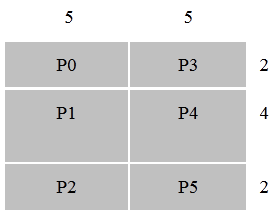
\includegraphics{create-irreg}
\centering
\caption{Creating an Irregular Array}
\label{crirreg}
\end{figure}

Return value: a non-zero array handle means the call was succesful.

\end{desc}

\seealso{CREATE,SET IRREG DISTR}


\apih{CREATE IRREG CONFIG}{Create an irregular-distributed GA with a specific configuration}

\begin{capi}
\begin{ccode}
int NGA_Create_irreg_config(int type, int ndim, int dims[],
                            char *array_name, int block[], int map[],
                            int p_handle)
\end{ccode}
\begin{funcargs}
\inarg{char*}{array_name}{a unique character string}
\inarg{int}{type}{MA data type (MT_F_DBL,MT_F_INT,MT_F_DCPL)}
\inarg{int}{ndim}{number of array dimensions}
\inarg{int*}{dims}{array of dimension values}
\inarg{int*}{nblock[ndim]}{no. of blocks each dimension is divided into}
\inarg{int*}{map[s]}{starting index for for each block; the size s is a sum all elements of nblock array}
\inarg{int}{p_handle}{processor list handle}
\outarg{int}{}{array handle}
\end{funcargs}
\end{capi}

\begin{fapi}
\begin{fcode}
logical function nga_create_irreg_config(type, ndim, dims, array_name,
                                         map, nblock, p_handle, g_a)
\end{fcode}
\begin{funcargs}
\inarg{character*(*)}{array_name}{a unique character string}
\inarg{integer}{type}{data type (MT_DBL,MT_INT,MT_DCPL)}
\inarg{integer}{ndim}{number of array dimensions}
\inarg{integer}{dims(ndim)}{array of dimensions}
\inarg{integer}{nblock(ndim)}{no. of blocks each dimension is divided into}
\inarg{integer}{map(s)}{starting index for for each block; the size s is a sum of all elements of nblock array}
\inarg{integer}{p_handle}{processor group handle}
\outarg{integer}{g_a}{integer handle for future references}
\end{funcargs}
\end{fapi}

\begin{cxxapi}
\begin{cxxcode}
GlobalArray::  GlobalArray(int type, int ndim, int dims[],
                           char *arrayname, int block[],
                           int maps[], PGroup* p_handle)
GlobalArray::  GlobalArray(int type, int ndim, int64_t dims[],
                           char *arrayname,
                           int64_t block[], int64_t maps[],
                           PGroup* p_handle)
\end{cxxcode}
\begin{funcargs}
\inarg{int}{type}{MA data type (MT_F_DBL,MT_F_INT,MT_F_DCPL)}
\inarg{int}{ndim}{number of array dimensions}
\inarg{int*}{dims}{array of dimension values}
\inarg{char*}{arrayname}{a unique character string}
\inarg{int*}{block[ndim]}{no. of blocks each dimension is divided into}
\inarg{int*}{maps[s]}{starting index for for each block; the size s is a sum all elements of nblock array}
\inarg{}{p_handle}{processor group handle}
\end{funcargs}
\end{cxxapi}

\begin{pyapi}
\begin{pycode}
g_a = ga.create_irreg(int gtype, dims, block, map, char *name='',
                      int pgroup=-1)
\end{pycode}
\begin{funcargs}
\inarg{int}{gtype}{data type (C_DBL,C_INT,C_DCPL)}
\inarg{1D array-like of ints}{dims}{array of dimension values}
\inarg{1D array-like of ints}{block}{no. of blocks each dimension is divided into}
\inarg{1D array-like of ints}{map}{starting index for for each block; len(map) is a sum all elements of block array}
\inarg{char*}{name}{a unique character string}
\inarg{int}{pgroup}{processor group handle}
\outarg{int}{}{array handle}
\end{funcargs}
\end{pyapi}

\dcoll

\begin{desc}

Creates an array by following the user-specified distribution and an explicitly
specified processor list handle and returns an integer handle representing the
array.

This call is essentially the same as the NGA_Create_irreg call, except for the
processor list handle p_handle. It can be used to create mirrored arrays.

Return value: a non-zero array handle means the call was succesful.

\end{desc}

\seealso{CREATE,SET IRREG DISTR, SET PGROUP}

\apih{CREATE GHOST IRREG}{Create an irregular-distributed GA with ghost cells}

\begin{capi}
\begin{ccode}
int NGA_Create_ghost_irreg(int type, int ndim, int dims[], width[],
                           char *array_name, nblock[], map[])
\end{ccode}
\begin{funcargs}
\inarg{char*}{array_name}{a unique character string}
\inarg{int}{type}{data type (MT_DBL,MT_INT,MT_DCPL)}
\inarg{int}{ndim}{number of array dimensions}
\inarg{int*}{dims[ndim]}{array of dimensions}
\inarg{int*}{width[ndim]}{array of ghost cell widths}
\inarg{int*}{nblock[ndim]}{no. of blocks each dimension is divided into}
\inarg{int*}{map[s]}{starting index for for each block; the size     s is a sum of all elements of nblock array}
\outarg{int}{}{array handle}
\end{funcargs}
\end{capi}

\begin{fapi}
\begin{fcode}
logical function nga_create_ghosts_irreg(type, ndim, dims, width, array_name, map, nblock, g_a)
\end{fcode}
\begin{funcargs}
\inarg{character*(*)}{array_name}{a unique character string}
\inarg{integer}{type}{data type (MT_DBL,MT_INT,MT_DCPL)}
\inarg{integer}{ndim}{number of array dimensions}
\inarg{integer}{dims(ndim)}{array of dimensions}
\inarg{integer}{width(ndim)}{array of ghost cell widths}
\inarg{integer}{nblock(ndim)}{no. of blocks each dimension is divided into}
\inarg{integer}{map(s)}{starting index for for each block; the size s is a sum of all elements of nblock array}
\outarg{integer}{g_a}{integer handle for future references}
\end{funcargs}
\end{fapi}

\begin{cxxapi}
\begin{cxxcode}
GlobalArray::GlobalArray(int type, int ndim, int dims[], int width[],
                         char *arrayname,
                         int block[], int maps[], char ghosts);
GlobalArray::GlobalArray(int type, int ndim, int64_t dims[],
                         int64_t width[], char *arrayname,
                         int64_t block[], int64_t maps[], char ghosts)
\end{cxxcode}
\begin{funcargs}
\inarg{int}{type}{data type (MT_DBL,MT_INT,MT_DCPL)}
\inarg{int}{ndim}{number of array dimensions}
\inarg{int*}{dims[ndim]}{array of dimensions}
\inarg{int*}{width[ndim]}{array of ghost cell widths}
\inarg{char*}{arrayname}{a unique character string}
\inarg{int*}{block[ndim]}{no. of blocks each dimension is divided into}
\inarg{int*}{maps[s]}{starting index for for each block; the size s is a sum of all elements of nblock array}
\inarg{char}{ghosts}{this is a dummy parameter: added to increase the number of arguments, inorder to avoid the conflicts among constructors. (ghosts = 'g' or 'G')}
\end{funcargs}
\end{cxxapi}

\begin{pyapi}
\begin{pycode}
g_a = ga.create_ghosts_irreg(int gtype, dims, width, block, map,
                             char *name='')
\end{pycode}
\begin{funcargs}
\inarg{int}{gtype}{data type (C_DBL,C_INT,C_DCPL)}
\inarg{1D array-like of ints}{dims}{array shape}
\inarg{1D array-like of ints}{width}{ghost cell widths per dimension}
\inarg{1D array-like of ints}{block}{no. of blocks each dimension is divided into}
\inarg{1D array-like of ints}{map}{starting index for for each block; len(map) is a sum all elements of block array}
\inarg{char*}{name}{a unique character string}
\outarg{int}{}{array handle}
\end{funcargs}
\end{pyapi}

\dcoll

\begin{desc}

Creates an array with ghost cells by following the user-specified distribution
and returns an integer handle representing the array.

The distribution is specified as a Cartesian product of distributions for each
dimension.

Figure \ref{crghostir} demonstrates distribution of a 2-dimensional array 8x10
on 6 (or more) processors.

nblock(2)=\{3,2\}, the size of map array is s=5 and the array map contains the
following elements map=\{1,3,7, 1, 6\}. The distribution is nonuniform because,
P1 and P4 get 20 elements each and processors P0, P2, P3, and P5 only 10
elements each.

The array width[] is used to control the width of the ghost cell boundary
around the visible data on each processor. The local data of the Global Array
residing on each processor will have a layer width[n] ghosts cells wide on
either side of the visible data along the dimension n.

Return value: a non-zero array handle means the call was succesful.

\begin{figure}
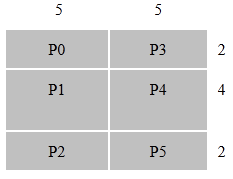
\includegraphics{create-ghosts-irreg}
\centering
\caption{Creating an Array with Ghost Cells}
\label{crghostir}
\end{figure}

\end{desc}

\seealso{CREATE,SET GHOSTS,SET IRREG DISTR}

\apih{CREATE GHOSTS IRREG CONFIG}{Create an irregular-distributed GA with ghost cells and a specific configuration}

\begin{capi}
\begin{ccode}
int NGA_Create_ghost_irreg_config(int type, int ndim, int dims[],
                                  width [], char*array_name,nblock[],
                                  map[], int p_handle)
\end{ccode}
\begin{funcargs}
\inarg{char*}{array_name}{a unique character string}
\inarg{int}{type}{data type (MT_DBL,MT_INT,MT_DCPL)}
\inarg{int}{ndim}{number of array dimensions}
\inarg{int*}{dims[ndim]}{array of dimensions}
\inarg{int*}{width[ndim]}{array of ghost cell widths}
\inarg{int*}{nblock[ndim]}{no. of blocks each dimension is divided into}
\inarg{int*}{map[s]}{starting index for for each block; the size s is a sum of all elements of nblock array}
\inarg{int}{p_handle}{processor list handle}
\end{funcargs}
\end{capi}

\begin{fapi}
\begin{fcode}
logical function nga_create_ghosts_irreg_config(type, ndim,
                                                dims, width, array_name,
                                                map, nblock,
                                                p_handle, g_a)
\end{fcode}
\begin{funcargs}
\inarg{character*(*)}{array_name}{a unique character string}
\inarg{integer}{type}{data type (MT_DBL,MT_INT,MT_DCPL)}
\inarg{integer}{ndim}{number of array dimensions}
\inarg{integer}{dims(ndim)}{array of dimensions}
\inarg{integer}{width(ndim)}{array of ghost cell widths}
\inarg{integer}{nblock(ndim)}{no. of blocks each dimension is divided into}
\inarg{integer}{map(s)}{starting index for for each block; the size s is a sum of all elements of nblock array}
\inarg{integer}{p_handle}{processor group handle}
\outarg{integer}{g_a}{integer handle for future references}
\end{funcargs}
\end{fapi}

\begin{cxxapi}
\begin{cxxcode}
GlobalArray::GlobalArray(int type, int ndim, int dims[], int width[],
                         char *arrayname, int block[], int maps[],
                         PGroup* p_handle, char ghosts)
GlobalArray::GlobalArray(int type, int ndim, int64_t dims[],
                         int64_t width[], char *arrayname,
                         int64_t block[], int64_t maps[],
                         PGroup* p_handle,char ghosts)
\end{cxxcode}
\begin{funcargs}
\inarg{int}{type}{data type (MT_DBL,MT_INT,MT_DCPL)}
\inarg{int}{ndim}{number of array dimensions}
\inarg{int*}{dims[ndim]}{array of dimensions}
\inarg{int*}{width[ndim]}{array of ghost cell widths}
\inarg{char*}{arrayname}{a unique character string}
\inarg{int*}{block[ndim]}{no. of blocks each dimension is divided into}
\inarg{int*}{maps[s]}{starting index for for each block; the size s is a sum of all elements of nblock array}
\inarg{PGroup*}{p_handle}{processor group handle}
\inarg{char}{ghosts}{this is a dummy parameter: added to increase the number of arguments, inorder to avoid the conflicts among constructors. (ghosts = 'g' or 'G')}
\end{funcargs}
\end{cxxapi}

\begin{pyapi}
\begin{pycode}
g_a = ga.create_ghosts_irreg(int gtype, dims, width, block, map,
                             char *name='', int pgroup=-1)
\end{pycode}
\begin{funcargs}
\inarg{int}{gtype}{data type (C_DBL,C_INT,C_DCPL)}
\inarg{1D array-like of ints}{dims}{array shape}
\inarg{1D array-like of ints}{width}{ghost cell widths per dimension}
\inarg{1D array-like of ints}{block}{no. of blocks each dimension is divided into}
\inarg{1D array-like of ints}{map}{starting index for for each block; len(map) is a sum all elements of block array}
\inarg{char*}{name}{a unique character string}
\inarg{int}{pgroup}{processor group handle}
\outarg{int}{}{array handle}
\end{funcargs}
\end{pyapi}

\dcoll

\begin{desc}

Creates an array with ghost cells by following the user-specified distribution
and returns integer handle representing the array.

This call is essentially the same as the NGA_Create_ghosts_irreg call, except
for the processor list handle p_handle. It can be used to create mirrored
arrays.

Return value: a non-zero array handle means the call was succesful.

\end{desc}

\seealso{CREATE,SET GHOSTS,SET IRREG DISTR,SET PGROUP}

\apih{CREATE HANDLE}{Create a handle to a global array}

\begin{capi}
\begin{ccode}
int GA_Create_handle()
\end{ccode}
\end{capi}

\begin{fapi}
\begin{fcode}
integer function ga_create_handle()
\end{fcode}
\end{fapi}

\begin{cxxapi}
\begin{cxxcode}
GlobalArray::GlobalArray()
\end{cxxcode}
\end{cxxapi}

\begin{pyapi}
\begin{pycode}
ret = ga.create_handle()
\end{pycode}
\end{pyapi}

\dcoll

\begin{desc}

This function returns a Global Array handle that can then be used to create a
new Global Array. This is part of a new API for creating Global Arrays that is
designed to replace the old interface built around the NGA_Create_xxx calls.
The sequence of operations is to begin with a call to GA_Greate_handle to get a
new array handle. The attributes of the array, such as dimension, size, type,
etc., can then be set using successive calls to the GA_Set_xxx subroutines.
When all array attributes have been set, the GA_Allocate subroutine is called
and the Global Array is actually created and memory for it is allocated.

\end{desc}


\apih{SET ARRAY NAME}{Set the array name for a GA handle}

\begin{capi}
\begin{ccode}
void GA_Set_array_name (int g_a, char *name)
\end{ccode}
\begin{funcargs}
\inarg{int}{g_a}{array handle}
\inarg{char*}{name}{array name}
\end{funcargs}
\end{capi}

\begin{fapi}
\begin{fcode}
subroutine ga_set_array_name(g_a, name)
\end{fcode}
\begin{funcargs}
\inarg{integer}{g_a}{global array handle}
\inarg{character*(*)}{name}{a unique character string}
\end{funcargs}
\end{fapi}

\begin{cxxapi}
\begin{cxxcode}
void GlobalArray::setArrayName(char *name) const
\end{cxxcode}
\begin{funcargs}
\inarg{char*}{name}{array name}
\end{funcargs}
\end{cxxapi}

\begin{pyapi}
\begin{pycode}
ga.set_array_name(int g_a, char *name)
\end{pycode}
\begin{funcargs}
\inarg{int}{g_a}{array handle}
\inarg{char*}{name}{array name}
\end{funcargs}
\end{pyapi}

\gcoll

\begin{desc}

This function can be used to assign a unique character string name to a Global
Array handle that was obtained using the GA_Create_handle function.

\end{desc}


\apih{SET DATA}{Set the data properties for a GA handle}

\begin{capi}
\begin{ccode}
void GA_Set_data (int g_a, int ndim, int dims[], int type)
\end{ccode}
\begin{funcargs}
\inarg{int}{g_a}{array handle}
\inarg{int}{ndim}{dimension of global array}
\inarg{int*}{dims[]}{dimensions of global array}
\inarg{int}{type}{data type of global array}
\end{funcargs}
\end{capi}

\begin{fapi}
\begin{fcode}
subroutine ga_set_data (g_a, ndim, dims, type)
\end{fcode}
\begin{funcargs}
\inarg{integer}{g_a}{global array handle}
\inarg{integer}{ndim}{dimension of array}
\inarg{integer}{dims(ndim)}{array dimensions}
\inarg{integer}{type}{data type (MT_DBL,MT_INT,etc.)}
\end{funcargs}
\end{fapi}

\begin{cxxapi}
\begin{cxxcode}
void GlobalArray::setData(int ndim, int dims[], int type) const
void GlobalArray::setData(int ndim, int64_t dims[], int type) const
\end{cxxcode}
\begin{funcargs}
\inarg{int}{ndim}{dimension of global array}
\inarg{int*}{dims}{dimensions of global array}
\inarg{int}{type}{data type of global array}
\end{funcargs}
\end{cxxapi}

\begin{pyapi}
\begin{pycode}
ga.set_data(int g_a, dims, int type)
\end{pycode}
\begin{funcargs}
\inarg{int}{g_a}{array handle}
\inarg{1D array-like of ints}{dims}{shape of global array}
\inarg{int}{type}{data type of global array}
\end{funcargs}
\end{pyapi}

\gcoll

\begin{desc}

This function can be used to set the array dimension, the coordinate
dimensions, and the data type assigned to a Global Array handle obtained using
the GA_Create_handle function.

\end{desc}


\apih{SET IRREG DISTR}{Specify irregular distribution for a GA handle}

\begin{capi}
\begin{ccode}
void GA_Set_irreg_distr(int g_a, int mapc[], int nblock[])
\end{ccode}
\begin{funcargs}
\inarg{int}{g_a}{array handle}
\inarg{int*}{mapc[s]}{starting index for each block; the size s is the sum of all elements of the array nblock}
\inarg{int*}{nblock[ndim]}{number of blocks that each dimension is divided into}
\end{funcargs}
\end{capi}

\begin{fapi}
\begin{fcode}
subroutine ga_set_irreg_distr(g_a, mapc, nblock)
\end{fcode}
\begin{funcargs}
\inarg{integer}{g_a}{global array handle}
\inarg{integer}{map(s)}{starting index for for each block; the size s is a sum of all elements of nblock array}
\inarg{integer}{nblock(ndim)}{no. of blocks each dimension is divided into}
\end{funcargs}
\end{fapi}

\begin{cxxapi}
\begin{cxxcode}
void GlobalArray::setIrregDistr(int mapc[], int nblock[]) const
void GlobalArray::setIrregDistr(int64_t mapc[], int64_t nblock[]) const
\end{cxxcode}
\begin{funcargs}
\inarg{}{mapc[s]}{starting index for each block; the size s is the sum of all elements of the array nblock}
\inarg{}{nblock[ndim]}{number of blocks that each dimension is divided into}
\end{funcargs}
\end{cxxapi}

\begin{pyapi}
\begin{pycode}
ga.set_irreg_distr(int g_a, mapc, nblock)
\end{pycode}
\begin{funcargs}
\inarg{int}{g_a}{array handle}
\inarg{1D array-like of ints}{mapc}{starting index for for each block; len(map) is a sum all elements of block array}
\inarg{1D array-like of ints}{nblock}{no. of blocks each dimension is divided into}
\end{funcargs}
\end{pyapi}

\gcoll

\begin{desc}

This function can be used to partition the array data among the individual
processors for a global array handle obtained using the GA_Create_handle
function.

The distribution is specified as a Cartesian product of distributions for each
dimension. For example, the following figure demonstrates distribution of a
2-dimensional array 8x10 on 6 (or more) processors. nblock(2)=\{3,2\}, the size
of mapc array is s=5 and array mapc contains the following elements mapc=\{1,
3, 7, 1, 6\}. The distribution is nonuniform because, P1 and P4 get 20 elements
each and processors P0, P2, P3, and P5 only 10 elements each.

The array width() is used to control the width of the ghost cell boundary
around the visible data on each processor. The local data of the global array
residing on each processor will have a layer width(n) ghosts cells wide on
either side of the visible data along the dimension n.

An example is shown in Figure \ref{setirregdist}.

\begin{figure}
\centering
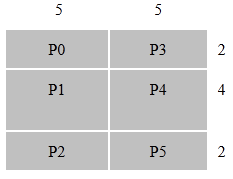
\includegraphics{set-irreg-dist}
\caption{Set an Irregular Distribution}
\label{setirregdist}
\end{figure}

\end{desc}

\apih{SET PGROUP}{Set the processor group for a GA handle}

\begin{capi}
\begin{ccode}
void GA_Set_pgroup(int g_a, int p_handle)
\end{ccode}
\begin{funcargs}
\inarg{int}{g_a}{array handle}
\inarg{int}{p_handle}{processor group handle}
\end{funcargs}
\end{capi}

\begin{fapi}
\begin{fcode}
subroutine ga_set_pgroup(g_a, p_handle)
\end{fcode}
\begin{funcargs}
\inarg{integer}{g_a}{global array handle}
\inarg{integer}{p_handle}{processor group handle}
\end{funcargs}
\end{fapi}

\begin{cxxapi}
\begin{cxxcode}
void GlobalArray::setPGroup(PGroup *pHandle) const
\end{cxxcode}
\begin{funcargs}
\inarg{PGroup*}{pHandle}{processor group instance}
\end{funcargs}
\end{cxxapi}

\begin{pyapi}
\begin{pycode}
ga.set_pgroup(int g_a, int pgroup)
\end{pycode}
\begin{funcargs}
\inarg{int}{g_a}{array handle}
\inarg{int}{p_handle}{processor group handle}
\end{funcargs}
\end{pyapi}

\gcoll

\begin{desc}

This function can be used to set the processor configuration assigned to a
global array handle that was obtained using the GA_Create_handle function. It
can be used to create mirrored arrays by using the mirrored array processor
configuration in this function call. It can also be used to create an array on
a processor group by using a processor group handle in this call.

\end{desc}

\apih{SET RESTRICTED}{Specify a GA handle to be allocated on a subset of processors}

\begin{capi}
\begin{ccode}
void GA_Set_restricted(int g_a, int list[], int nproc)
\end{ccode}
\begin{funcargs}
\inarg{int}{g_a}{global array handle}
\inarg{int*}{list[nproc]}{list of processor IDs that contain data}
\inarg{int}{nproc}{number of processors that contain data}
\end{funcargs}
\end{capi}

\begin{fapi}
\begin{fcode}
subroutine ga_set_restricted(g_a, list, nproc)
\end{fcode}
\begin{funcargs}
\inarg{integer}{g_a}{global array handle}
\inarg{integer}{list(nproc)}{list of processor IDs that contain data}
\inarg{integer}{nproc}{number of processors that contain data}
\end{funcargs}
\end{fapi}

\begin{cxxapi}
\begin{cxxcode}
void GlobalArray::setRestricted(int list[], int nprocs) const
\end{cxxcode}
\begin{funcargs}
\inarg{int*}{list}{list of processors that should contain data}
\inarg{int}{nprocs}{number of processors in list}
\end{funcargs}
\end{cxxapi}

\begin{pyapi}
\begin{pycode}
ga.set_restricted(int g_a, list)
\end{pycode}
\begin{funcargs}
\inarg{int}{g_a}{global array handle}
\inarg{1D array-like of ints}{list}{list of processor IDs that contain data}
\end{funcargs}
\end{pyapi}

\gcoll

\begin{desc}

This function restricts data in the global array g_a to only the nproc
processors listed in the array list. The value of nproc must be less than or
equal to the number of available processors. If this call is used in
conjunction with GA_Set_irreg_distr, then the decomposition in the
GA_Set_irreg_distr call must be done assuming that the number of processors is
nproc. The data that ordinarily would be mapped to process 0 is mapped to the
process in list[0], the data that would be mapped to process 1 will be mapped
to list[1], etc. This can be used to remap the data distribution to different
processors, even if nproc equals the number of available processors.

\end{desc}

\apih{SET RESTRICTED RANGE}{Specify a GA handle to be created on a subset (as a range) of processors}

\begin{capi}
\begin{ccode}
void GA_set_restricted_range(int g_a, int lo_proc, int hi_proc)
\end{ccode}
\begin{funcargs}
\inarg{int}{g_a}{global array handle}
\inarg{int}{lo_proc}{range of processors (inclusive) that contain data}
\inarg{int}{hi_proc}{range of processors (inclusive) that contain data}
\end{funcargs}
\end{capi}

\begin{fapi}
\begin{fcode}
subroutine ga_set_restricted_range(g_a, lo_proc, hi_proc)
\end{fcode}
\begin{funcargs}
\inarg{integer}{g_a}{global array handle}
\inarg{integer}{lo_proc}{range of processors (inclusive) that contain data}
\inarg{integer}{hi_proc}{range of processors (inclusive) that contain data}
\end{funcargs}
\end{fapi}

\begin{cxxapi}
\begin{cxxcode}
void GlobalArray::setRestrictedRange(int lo_proc, int hi_proc) const
\end{cxxcode}
\begin{funcargs}
\inarg{int}{lo_proc}{low end of processor range}
\inarg{int}{hi_proc}{high end of processor range}
\end{funcargs}
\end{cxxapi}

\begin{pyapi}
\begin{pycode}
ga.set_restricted_range(int g_a, int lo_proc, int hi_proc)
\end{pycode}
\begin{funcargs}
\inarg{int}{g_a}{global array handle}
\inarg{int}{lo_proc}{range of processors (inclusive) that contain data}
\inarg{int}{hi_proc}{range of processors (inclusive) that contain data}
\end{funcargs}
\end{pyapi}

\gcoll

\begin{desc}

This function restricts data in the global array to the range of processors
beginning with lo_proc and ending with hi_proc. Both lo_proc and hi_proc must
be less than or equal to the total number of processors minus one (e.g., in the
range [0,N-1], where N is the total number of processors) and lo_proc must be
less than or equal to hi_proc. If lo_proc = 0 and hi_proc = N-1 then this call
has no effect on the data distribution.

\end{desc}

\apih{SET GHOSTS}{Specify ghost cells for a GA handle}

\begin{capi}
\begin{ccode}
void GA_Set_ghosts(int g_a, int width[])
\end{ccode}
\begin{funcargs}
\inarg{int}{g_a}{array handle}
\inarg{int*}{width[ndim]}{array of ghost cell widths}
\end{funcargs}
\end{capi}

\begin{fapi}
\begin{fcode}
subroutine ga_set_ghosts(g_a, width)
\end{fcode}
\begin{funcargs}
\inarg{integer}{g_a}{global array handle}
\inarg{integer}{width(ndim)}{array of ghost cell widths}
\end{funcargs}
\end{fapi}

\begin{cxxapi}
\begin{cxxcode}
void GlobalArray::setGhosts(int width[]) const
void GlobalArray::setGhosts(int64_t width[]) const
\end{cxxcode}
\begin{funcargs}
\inarg{}{width[ndim]}{array of ghost cell widths}
\end{funcargs}
\end{cxxapi}

\begin{pyapi}
\begin{pycode}
ga.set_ghosts(int g_a, width)
\end{pycode}
\begin{funcargs}
\inarg{int}{g_a}{array handle}
\inarg{1D array-like of ints}{width}{ghost cell widths}
\end{funcargs}
\end{pyapi}

\gcoll

\begin{desc}

This function can be used to set the ghost cell widths for a global array
handle that was obtained using the GA_Create_handle function.  The ghosts cells
widths indicate how many ghost cells are used to pad the locally held array
data along each dimension. The padding can be set independently for each
coordinate dimension.

\end{desc}

\apih{SET CHUNK}{Specify chunk size for a GA handle}

\begin{capi}
\begin{ccode}
void GA_Set_chunk(int g_a, int chunk[])
\end{ccode}
\begin{funcargs}
\inarg{int}{g_a}{array handle}
\inarg{int*}{chunk[]}{array of chunk widths}
\end{funcargs}
\end{capi}

\begin{fapi}
\begin{fcode}
subroutine ga_set_chunk(g_a, chunk)
\end{fcode}
\begin{funcargs}
\inarg{integer}{g_a}{global array handle}
\inarg{integer}{chunk(ndim)}{array of chunk widths}
\end{funcargs}
\end{fapi}

\begin{cxxapi}
\begin{cxxcode}
void GlobalArray::setChunk(int chunk[]) const
void GlobalArray::setChunk(int64_t chunk[]) const
\end{cxxcode}
\begin{funcargs}
\inarg{int*}{chunk}{array of chunk widths}
\end{funcargs}
\end{cxxapi}

\begin{pyapi}
\begin{pycode}
ga.set_chunk(int g_a, chunk)
\end{pycode}
\begin{funcargs}
\inarg{int}{g_a}{array handle}
\inarg{1D array-like of ints}{chunk}{chunk widths}
\end{funcargs}
\end{pyapi}

\gcoll

\begin{desc}

This function is used to set the chunk array for a global array handle that was
obtained using the GA_Create_handle function. The chunk array is used to
determine the minimum number of array elements assigned to each processor along
each coordinate direction.

\end{desc}

\apih{SET BLOCK CYCLIC}{Specify round-robin distribution for a GA handle}

\begin{capi}
\begin{ccode}
void GA_Set_block_cyclic(int g_a, int dims[])
\end{ccode}
\begin{funcargs}
\inarg{int}{g_a}{global array handle}
\inarg{int*}{dims[]}{array of block dimensions}
\end{funcargs}
\end{capi}

\begin{fapi}
\begin{fcode}
subroutine ga_set_block_cyclic(g_a, dims)
\end{fcode}
\begin{funcargs}
\inarg{integer}{g_a}{global array handle}
\inarg{integer}{dims(ndim)}{array of block dimensions}
\end{funcargs}
\end{fapi}

\begin{cxxapi}
\begin{cxxcode}
void GlobalArray::setBlockCyclic(int dims[]) const
\end{cxxcode}
\begin{funcargs}
\inarg{int*}{dims}{array of block dimensions}
\end{funcargs}
\end{cxxapi}

\begin{pyapi}
\begin{pycode}
ga.set_block_cyclic(int g_a, dims)
\end{pycode}
\begin{funcargs}
\inarg{int}{g_a}{global array handle}
\inarg{1D array-like of ints}{dims}{block dimensions}
\end{funcargs}
\end{pyapi}

\gcoll

\begin{desc}

This subroutine is used to create a global array with a simple block-cyclic
data distribution. The array is broken up into blocks of size dims and each
block is numbered sequentially using a column major indexing scheme. The blocks
are then assigned in a simple round-robin fashion to processors.

Figure \ref{stblkcy} illustrates an array containing 25 blocks distributed on 4
processors.

Blocks at the edge of the array may be smaller than the block size specified in
dims. In the example below, blocks 4, 9, 14, 19, 20, 21, 22, 23, and 24 might
be smaller than the remaining blocks. Most global array operations are
insensitive to whether or not a block-cyclic data distribution is used,
although performance may be slower in some cases if the global array is using a
block-cyclic data distribution. Individual data blocks can be accessesed using
the block-cyclic access functions.

\begin{figure}
\centering
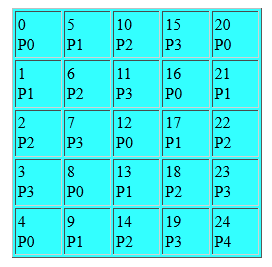
\includegraphics{set-block-cyclic}
\caption{Set Block Cyclic Data Distribution}
\label{stblkcy}
\end{figure}

\end{desc}

\apih{SET BLOCK CYCLIC PROC GRID}{Specify block-cyclic processor distribution for a GA handle}

\begin{capi}
\begin{ccode}
void GA_Set_block_cyclic(int g_a, int dims[], int proc_grid[])
\end{ccode}
\begin{funcargs}
\inarg{int}{g_a}{global array handle}
\inarg{int*}{dims[]}{array of block dimensions}
\inarg{int*}{proc_grid[]}{processor grid dimensions}
\end{funcargs}
\end{capi}

\begin{fapi}
\begin{fcode}
subroutine ga_set_block_cyclic_proc_grid(g_a, dims, proc_grid)
\end{fcode}
\begin{funcargs}
\inarg{integer}{g_a}{global array handle}
\inarg{integer}{dims(ndim)}{array of block dimensions}
\end{funcargs}
\end{fapi}

\begin{cxxapi}
\begin{cxxcode}
void GlobalArray::setBlockCyclicProcGrid(int dims[], int proc_grid[]) const
\end{cxxcode}
\begin{funcargs}
\inarg{int*}{dims}{array of block dimensions}
\inarg{int*}{proc_grid}{processor grid dimensions}
\end{funcargs}
\end{cxxapi}

\begin{pyapi}
\begin{pycode}
ga.set_block_cyclic_proc_grid(int g_a, block, proc_grid)
\end{pycode}
\begin{funcargs}
\inarg{int}{g_a}{global array handle}
\inarg{1D array-like of ints}{dims}{block dimensions}
\inarg{1D array-like of ints}{proc_grid}{processor grid dimensions}
\end{funcargs}
\end{pyapi}

\gcoll

\begin{desc}

This subroutine is used to create a global array with a SCALAPACK-type block
cyclic data distribution. The user specifies the dimensions of the processor
grid in the array proc_grid. The product of the processor grid dimensions must
equal the number of total number of processors and the number of dimensions in
the processor grid must be the same as the number of dimensions in the global
array. The data blocks are mapped onto the processor grid in a cyclic manner
along each of the processor grid axes.

Figure \ref{setblkcyprocgrid} illustrates an array consisting of 25 data blocks
distributed on 6 processors.

The 6 processors are configured in a 3 by 2 processor grid. Blocks at the edge
of the array may be smaller than the block size specified in dims.  Most global
array operations  are insensitive to whether or not a block-cyclic data
distribution is used, although performance may be slower in some cases if the
global array is using a block-cyclic data distribution. Individual data blocks
can be accessesed using the block-cyclic access functions.

\begin{figure}
\centering
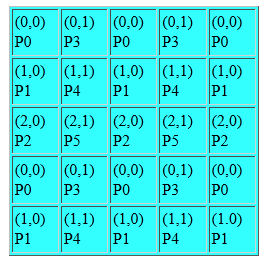
\includegraphics{set-block-cyclic-proc-grid}
\caption{Creating a SCALAPACK-type Block Cyclic Data Distribution}
\label{setblkcyprocgrid}
\end{figure}

\end{desc}

\apih{ALLOCATE}{Allocate the array specified by a GA handle}

\begin{capi}
\begin{ccode}
int GA_Allocate(int g_a)
\end{ccode}
\begin{funcargs}
\inarg{int}{g_a}{array handle}
\outarg{int}{}{1 if allocation of g_a was successful}
\end{funcargs}
\end{capi}

\begin{fapi}
\begin{fcode}
logical function ga_allocate(g_a)
\end{fcode}
\begin{funcargs}
\inarg{integer}{g_a}{global array handle}
\outarg{logical}{}{.TRUE. if allocation of g_a was successful}
\end{funcargs}
\end{fapi}

\begin{cxxapi}
\begin{cxxcode}
int GlobalArray::allocate() const
\end{cxxcode}
\end{cxxapi}

\begin{pyapi}
\begin{pycode}
ret = ga.allocate(int g_a)
\end{pycode}
\begin{funcargs}
\inarg{int}{g_a}{array handle}
\outarg{bool}{ret}{True if allocation of g_a was successful}
\end{funcargs}
\end{pyapi}

\gcoll

\begin{desc}

This function allocates the memory for the global array handle originally
obtained using the GA_Create_handle function. At a minimum, the GA_Set_data
function must be called before the memory is allocated. Other GA_Set_xxx
functions can also be called before invoking this function.

Returns True if allocation of g_a was successful.

\end{desc}

\apih{UPDATE GHOSTS}{Update ghost cells}

\begin{capi}
\begin{ccode}
void GA_Update_ghosts(int g_a)
\end{ccode}
\begin{funcargs}
\inarg{int}{g_a}{array handle}
\end{funcargs}
\end{capi}

\begin{fapi}
\begin{fcode}
subroutine ga_update_ghosts(g_a)
\end{fcode}
\begin{funcargs}
\inarg{integer}{g_a}{array handle}
\end{funcargs}
\end{fapi}

\begin{cxxapi}
\begin{cxxcode}
void GlobalArray::updateGhosts() const
\end{cxxcode}
\end{cxxapi}

\begin{pyapi}
\begin{pycode}
ga.update_ghosts(int g_a)
\end{pycode}
\begin{funcargs}
\inarg{int}{g_a}{array handle}
\end{funcargs}
\end{pyapi}

\gcoll

\begin{desc}

This call updates the ghost cell regions on each processor with the
corresponding neighbor data from other processors. The operation assumes that
all data is wrapped around using periodic boundary data so that ghost cell data
that goes beyound an array boundary is wrapped around to the other end of the
array. The GA_Update_ghosts call contains two GA_Sync calls before and after
the actual update operation. For some applications these calls may be
unecessary, if so they can be removed using the GA_Mask_sync subroutine.

\end{desc}

\apih{UPDATE GHOST DIR}{Update ghost cells along a specific direction}

\begin{capi}
\begin{ccode}
int NGA_Update_ghost_dir(int g_a, int dimension, int idir, int cflag)
\end{ccode}
\begin{funcargs}
\inarg{int}{g_a}{array handle}
\inarg{int}{dimension}{array dimension that is to be updated}
\inarg{int}{idir}{direction of update (+/- 1)}
\inarg{int}{cflag}{flag (0/1) to include corners in update}
\end{funcargs}
\end{capi}

\begin{fapi}
\begin{fcode}
logical function nga_update_ghost_dir(g_a,dimension,idir,cflag)
\end{fcode}
\begin{funcargs}
\inarg{integer}{g_a}{array handle}
\inarg{integer}{dimension}{array dimension that is to be updated}
\inarg{integer}{idir}{direction of update (+/-1)}
\inarg{logical}{cflag}{flag to include corners in update}
\end{funcargs}
\end{fapi}

\begin{cxxapi}
\begin{cxxcode}
int GlobalArray::updateGhostDir(int dimension, int idir, int cflag) const
\end{cxxcode}
\begin{funcargs}
\inarg{int}{dimension}{array dimension that is to be updated}
\inarg{int}{idir}{direction of update (+/- 1)}
\inarg{int}{cflag}{flag (0/1) to include corners in update}
\end{funcargs}
\end{cxxapi}

\begin{pyapi}
\begin{pycode}
ga.update_ghost_dir(int g_a, int dimension, int dir, int flag)
\end{pycode}
\begin{funcargs}
\inarg{int}{g_a}{array handle}
\inarg{int}{dimension}{array dimension that is to be updated}
\inarg{int}{dir}{direction of update (+/- 1)}
\inarg{int}{flag}{flag (0/1) to include corners in update}
\end{funcargs}
\end{pyapi}

\gcoll

\begin{desc}

This function can be used to update the ghost cells along individual
directions. It is designed for algorithms that can overlap updates with
computation. The variable dimension indicates which coordinate direction is to
be updated (e.g. dimension = 1 would correspond to the y axis in a two or three
dimensional system), the variable idir can take the values +/-1 and indicates
whether the side that is to be updated lies in the positive or negative
direction, and cflag indicates whether or not the corners on the side being
updated are to be included in the update. The following calls would be
equivalent to a call to GA_Update_ghosts for a 2-dimensional system:

\begin{verbatim}
     status = NGA_Update_ghost_dir(g_a,0,-1,1);
     status = NGA_Update_ghost_dir(g_a,0,1,1);
     status = NGA_Update_ghost_dir(g_a,1,-1,0);
     status = NGA_Update_ghost_dir(g_a,1,1,0);
\end{verbatim}

The variable cflag is set equal to 1 (or non-zero) in the first two calls so
that the corner ghost cells are update, it is set equal to 0 in the second two
calls to avoid redundant updates of the corners. Note that updating the ghosts
cells using several independent calls to the nga_update_ghost_dir functions is
generally not as efficient as using GA_Update_ghosts unless the individual
calls can be effectively overlapped with computation.

\end{desc}

\apih{HAS GHOSTS}{Check whether a GA has ghost cells}

\begin{capi}
\begin{ccode}
int GA_Has_ghosts(int g_a)
\end{ccode}
\begin{funcargs}
\inarg{int}{g_a}{array handle}
\outarg{int}{}{1 if array has ghost cells}
\end{funcargs}
\end{capi}

\begin{fapi}
\begin{fcode}
logical function ga_has_ghosts(g_a)
\end{fcode}
\begin{funcargs}
\inarg{integer}{g_a}{array handle}
\outarg{logical}{}{.TRUE. if array has ghost cells}
\end{funcargs}
\end{fapi}

\begin{cxxapi}
\begin{cxxcode}
int GlobalArray::hasGhosts() const
\end{cxxcode}
\begin{funcargs}
\outarg{int}{}{1 if array has ghost cells}
\end{funcargs}
\end{cxxapi}

\begin{pyapi}
\begin{pycode}
ret = ga.has_ghosts(int g_a)
\end{pycode}
\begin{funcargs}
\inarg{int}{g_a}{array handle}
\outarg{int}{ret}{True if array has ghost cells}
\end{funcargs}
\end{pyapi}

\gcoll

\begin{desc}

This function returns 1 if the global array has some dimensions for which the
ghost cell width is greater than zero, it returns 0 otherwise.

\end{desc}

\apih{ACCESS GHOSTS}{Access the ghost cells allocated locally on a GA}

\begin{capi}
\begin{ccode}
void NGA_Access_ghosts(int g_a, int dims[], void *ptr, int ld[])
\end{ccode}
\begin{funcargs}
\inarg{int}{g_a}{array handle}
\outarg{int*}{dims[ndim]}{array of dimensions of local patch, including ghost cells}
\outarg{void**}{ptr}{returns a pointer corresponding to the origin the global array patch held locally on the processor}
\outarg{int*}{ld[ndim-1]}{physical dimenstions of the local array patch, including ghost cells}
\end{funcargs}
\end{capi}

\begin{fapi}
\begin{fcode}
subroutine nga_access_ghosts(g_a, dims, index, ld)
\end{fcode}
\begin{funcargs}
\inarg{integer}{g_a}{array handle}
\outarg{integer}{dims(ndim)}{array of dimensions of local patch, including ghost cells}
\outarg{integer}{index}{returns an index corresponding to the origin the global array patch held locally on the processor}
\outarg{integer}{ld(ndim)}{physical dimenstions of the local array patch, including ghost cells}
\end{funcargs}
\end{fapi}

\begin{cxxapi}
\begin{cxxcode}
void GlobalArray::accessGhosts(int dims[], void *ptr, int ld[]) const
void GlobalArray::accessGhosts(int64_t dims[], void *ptr, int64_t ld[]) const
\end{cxxcode}
\begin{funcargs}
\outarg{int*}{dims[ndim]}{array of dimensions of local patch, including ghost cells}
\outarg{void**}{ptr}{returns an index corresponding to the origin the global array patch held locally on the processor}
\outarg{int*}{ld[ndim-1]}{physical dimensions of the local array patch, including ghost cells}
\end{funcargs}
\end{cxxapi}

\begin{pyapi}
\begin{pycode}
ret = ga.access_ghosts(int g_a)
\end{pycode}
\begin{funcargs}
\inarg{int}{g_a}{the array handle}
\outarg{ndarray}{ret}{appropriately shaped, possibly non-contiguous ndarray corresponding to global array patch held locally on the processor}
\end{funcargs}
\end{pyapi}

\local

\begin{desc}

Provides access to the local patch of the global array. Returns leading
dimension ld and and pointer for the data.  This routine will provide access to
the ghost cell data residing on each processor. Calls to NGA_Access_ghosts
should normally follow a call to NGA_Distribution that returns coordinates of
the visible data patch associated with a processor. You need to make sure that
the coordinates of the patch are valid (test values returned from
NGA_Distribution).

You can only access local data.

\end{desc}

\seealso{ACCESS,RELEASE GHOSTS,RELEASE UPDATE GHOSTS}

\apih{ACCESS GHOST ELEMENT}{Access a specific ghost element locally allocated on a GA}

\begin{capi}
\begin{ccode}
void NGA_Access_ghost_element(int g_a, void *ptr, int subscript[],
                              int ld[])
\end{ccode}
\begin{funcargs}
\inarg{int}{g_a}{array handle}
\outarg{void**}{ptr}{pointer to location of element indexed by subscript[]}
\inarg{int*}{subscript[ndim]}{array of integers that index desired element}
\outarg{int*}{ld[ndim-1]}{array of strides for local data patch.  These include ghost cell widths.}
\end{funcargs}
\end{capi}

\begin{fapi}
\begin{fcode}
subroutine nga_access_ghost_element(g_a, index, subscript, ld)
\end{fcode}
\begin{funcargs}
\inarg{integer}{g_a}{array handle}
\outarg{integer}{index}{index pointing to location of element indexed by subscript()}
\inarg{integer}{subscript(ndim)}{array of integers that index desired element}
\outarg{integer}{ld(ndim-1)}{array of strides for local data patch. These include ghost cell widths.}
\end{funcargs}
\end{fapi}

\begin{cxxapi}
\begin{cxxcode}
void GlobalArray::accessGhostElement(void *ptr, int subscript[],
                                     int ld[]) const
void GlobalArray::accessGhostElement(void *ptr, int64_t subscript[],
                                     int64_t ld[]) const
\end{cxxcode}
\begin{funcargs}
\outarg{void**}{ptr}{index pointing to location of element indexed by subscript[]}
\inarg{int*}{subscript[ndim]}{array of integers that index desired element}
\outarg{int*}{ld[ndim-1]}{array of strides for local data patch.  These include ghost cell widths.}
\end{funcargs}
\end{cxxapi}

\begin{pyapi}
\begin{pycode}
ret = ga.access_ghost_element(int g_a, subscript)
\end{pycode}
\begin{funcargs}
\inarg{int}{g_a}{the array handle}
\inarg{1D array-like of ints}{subscript}{index of desired element}
\outarg{ndarray}{ret}{appropriately shaped, possibly non-contiguous ndarray corresponding to global array patch held locally on the processor}
\end{funcargs}
\end{pyapi}

\local

\begin{desc}

This function can be used to return a pointer to any data element in the
locally held portion of the global array and can be used to directly access
ghost cell data. The array subscript refers to the local index of the element
relative to the origin of the local patch (which is assumed to be indexed by
(0,0,...)).

\end{desc}

\seealso{ACCESS,RELEASE GHOST ELEMENT,RELEASE UPDATE GHOST ELEMENT}

\apih{TOTAL BLOCKS}{Number of blocks allocated when using block-cyclic distribution}

\begin{capi}
\begin{ccode}
int GA_Total_blocks(int g_a)
\end{ccode}
\begin{funcargs}
\inarg{int}{g_a}{array handle}
\outarg{int}{}{total number of blocks in the block-cyclic distribution}
\end{funcargs}
\end{capi}

\begin{fapi}
\begin{fcode}
integer function ga_total_blocks(g_a)
\end{fcode}
\begin{funcargs}
\inarg{integer}{g_a}{array handle}
\outarg{integer}{}{total number of blocks in the block-cyclic distribution}
\end{funcargs}
\end{fapi}

\begin{cxxapi}
\begin{cxxcode}
int GlobalArray::totalBlocks() const
\end{cxxcode}
\begin{funcargs}
\outarg{int}{}{total number of blocks in the block-cyclic distribution}
\end{funcargs}
\end{cxxapi}

\begin{pyapi}
\begin{pycode}
ret = ga.total_blocks(int g_a)
\end{pycode}
\begin{funcargs}
\inarg{int}{g_a}{array handle}
\outarg{int}{ret}{total number of blocks in the block-cyclic distribution}
\end{funcargs}
\end{pyapi}

\local

\begin{desc}

This function returns the total number of blocks contained in a global array
with a block-cyclic data distribution.

\end{desc}

\seealso{SET BLOCK CYCLIC,SET BLOCK CYCLIC PROC GRID}

\apih{GET BLOCK INFO}{Information on block-cyclic information for a GA}

\begin{capi}
\begin{ccode}
void GA_Get_block_info(int g_a, int num_blocks[], int block_dims[])
\end{ccode}
\begin{funcargs}
\inarg{int}{g_a}{array handle}
\outarg{int*}{num_blocks[ndim]}{number of blocks along each axis}
\outarg{int*}{block_dims[ndim]}{dimensions of block}
\end{funcargs}
\end{capi}

\begin{fapi}
\begin{fcode}
subroutine ga_get_block_info(g_a, num_blocks, block_dims)
\end{fcode}
\begin{funcargs}
\inarg{integer}{g_a}{array handle}
\outarg{integer}{num_blocks(ndim)}{number of blocks along each axis}
\outarg{integer}{block_dims(ndim)}{dimensions of block}
\end{funcargs}
\end{fapi}

\begin{cxxapi}
\begin{cxxcode}
void GlobalArray::getBlockInfo(int num_blocks[], int block_dims[])
\end{cxxcode}
\begin{funcargs}
\outarg{int*}{num_blocks[ndim]}{array containing number of blocks along each coordinate direction}
\outarg{int*}{block_dims[ndim]}{array containing block dimensions}
\end{funcargs}
\end{cxxapi}

\begin{pyapi}
\begin{pycode}
num_blocks,block_dims = get_block_info(int g_a)
\end{pycode}
\begin{funcargs}
\inarg{int}{g_a}{array handle}
\outarg{1D ndarray of ints}{num_blocks}{number of blocks along each axis}
\outarg{1D ndarray of ints}{block_dims}{dimensions of block}
\end{funcargs}
\end{pyapi}

\local

\begin{desc}

This subroutine returns information about the block-cyclic distribution
associated with global array g_a. The number of blocks along each of the array
axes are returned in the array num_blocks and the dimensions of the individual
blocks, specified in the GA_Set_block_cyclic or GA_Set_block_cyclic_proc_grid
subroutines, are returned in block_dims.

This is a local function.

\end{desc}

\seealso{SET BLOCK CYCLIC,SET BLOCK CYCLIC PROC GRID}

\apih{DUPLICATE}{Duplicate a GA}

\begin{capi}
\begin{ccode}
int GA_Duplicate(int g_a, char* array_name)
\end{ccode}
\begin{funcargs}
\inarg{char*}{array_name}{a character string}
\inarg{int}{g_a}{integer handle for reference array}
\outarg{int}{}{integer handle for duplicated array}
\end{funcargs}
\end{capi}

\begin{fapi}
\begin{fcode}
logical function ga_duplicate(g_a, g_b, array_name)
\end{fcode}
\begin{funcargs}
\inarg{character*(*)}{array_name}{a character string}
\inarg{integer}{g_a}{Integer handle for reference array}
\outarg{integer}{g_b}{Integer handle for new array}
\outarg{logical}{}{.TRUE. if array creation successful}
\end{funcargs}
\end{fapi}

\begin{cxxapi}
\begin{cxxcode}
GlobalArray::GlobalArray(const GlobalArray &g_a, char *arrayname)
GlobalArray::GlobalArray(const GlobalArray &g_a)
GlobalArray * GAServices::createGA(const GlobalArray *g_b, char *arrayname)
GlobalArray * GAServices::createGA(const GlobalArray &g_b)
\end{cxxcode}
\begin{funcargs}
\inarg{int}{g_b}{integer handle for reference array}
\inarg{char*}{arrayname}{a character string}
\end{funcargs}
\end{cxxapi}

\begin{pyapi}
\begin{pycode}
ret = ga.duplicate(int g_a, char *name='')
\end{pycode}
\begin{funcargs}
\inarg{int}{g_a}{integer handle for reference array}
\inarg{char*}{array_name}{a character string}
\outarg{int}{ret}{integer handle for duplicated array}
\end{funcargs}
\end{pyapi}

\gcoll

\begin{desc}

Creates a new array by applying all the properties of another existing array.
It returns an array handle.

Return value: a non-zero array handle means the call was succesful.

\end{desc}

\apih{DESTROY}{Destroy a global array}

\begin{capi}
\begin{ccode}
void GA_Destroy(int g_a)
\end{ccode}
\begin{funcargs}
\inarg{int}{g_a}{array handle}
\end{funcargs}
\end{capi}

\begin{fapi}
\begin{fcode}
logical function ga_destroy(g_a)
\end{fcode}
\begin{funcargs}
\inarg{integer}{g_a}{array handle}
\end{funcargs}
\end{fapi}

\begin{cxxapi}
\begin{cxxcode}
GlobalArray::~GlobalArray()
void GlobalArray::destroy()
\end{cxxcode}
\end{cxxapi}

\begin{pyapi}
\begin{pycode}
ga.destroy(int g_a)
\end{pycode}
\begin{funcargs}
\inarg{int}{g_a}{array handle}
\end{funcargs}
\end{pyapi}

\gcoll

\begin{desc}

Deallocates the array and frees any associated resources.

\end{desc}

\apih{TERMINATE}{Terminate GA}

\begin{capi}
\begin{ccode}
void GA_Terminate()
\end{ccode}
\end{capi}

\begin{fapi}
\begin{fcode}
subroutine ga_terminate()
\end{fcode}
\end{fapi}

\begin{cxxapi}
\begin{cxxcode}
void GA::Terminate()
\end{cxxcode}
\end{cxxapi}

\begin{pyapi}
\begin{pycode}
ga.terminate()
\end{pycode}
\end{pyapi}

\wcoll

\begin{desc}

Delete all active arrays and destroy internal data structures.

\end{desc}

\begin{pydesc}

This functions is automatically called during atexit(). There is no need (and
is an error) to call this function explicitly.

\end{pydesc}

\apih{SYNC}{Synchronize all processes in the default processor group}

\begin{capi}
\begin{ccode}
void GA_Sync()
\end{ccode}
\end{capi}

\begin{fapi}
\begin{fcode}
subroutine ga_sync()
\end{fcode}
\end{fapi}

\begin{cxxapi}
\begin{cxxcode}
GAServices::sync()
GA::sync()
\end{cxxcode}
\end{cxxapi}

\begin{pyapi}
\begin{pycode}
ga.sync()
\end{pycode}
\end{pyapi}

\dcoll

\begin{desc}

Synchronize processes (a barrier) and ensure that all GA operations completed.

\end{desc}

\apih{MASK SYNC}{Mask GA synchronization operations}

\begin{capi}
\begin{ccode}
void GA_Mask_sync(int first, int last)
\end{ccode}
\begin{funcargs}
\inarg{int}{first}{mask (0/1) for prior internal synchronization}
\inarg{int}{last}{mask (0/1) for post internal synchronization}
\end{funcargs}
\end{capi}

\begin{fapi}
\begin{fcode}
subroutine ga_mask_sync(first,last)
\end{fcode}
\begin{funcargs}
\inarg{logical}{first}{mask for prior internal synchronization}
\inarg{logical}{last}{mask for post internal synchronization}
\end{funcargs}
\end{fapi}

\begin{cxxapi}
\begin{cxxcode}
void GAServices::maskSync(int first, int last)
void GA::maskSync(int first, int last)
\end{cxxcode}
\begin{funcargs}
\inarg{int}{first}{masks the sync at the begining of the collective call}
\inarg{int}{last}{masks the sync at the end of the collective call}
\end{funcargs}
\end{cxxapi}

\begin{pyapi}
\begin{pycode}
ga.mask_sync(int first, int last)
\end{pycode}
\end{pyapi}
\begin{funcargs}
\inarg{bool}{first}{mask for prior internal synchronization}
\inarg{bool}{last}{mask for post internal synchronization}
\end{funcargs}

\dcoll

\begin{desc}

This subroutine can be used to remove synchronization calls from around
collective operations. Setting the parameter first = .false. removes the
synchronization prior to the collective operation, setting last = .false.
removes the synchronization call after the collective operation. This call is
applicable to all collective operations.  It most be invoked before each
collective operation.

\end{desc}

\seealso{SYNC}

\apih{ZERO}{Zero a global array}

\begin{capi}
\begin{ccode}
void GA_Zero(int g_a)
\end{ccode}
\begin{funcargs}
\inarg{int}{g_a}{array handle}
\end{funcargs}
\end{capi}

\begin{fapi}
\begin{fcode}
subroutine ga_zero(g_a)
\end{fcode}
\begin{funcargs}
\inarg{integer}{g_a}{array handle}
\end{funcargs}
\end{fapi}

\begin{cxxapi}
\begin{cxxcode}
void GlobalArray::zero() const
\end{cxxcode}
\end{cxxapi}

\begin{pyapi}
\begin{pycode}
ga.zero(int g_a)
\end{pycode}
\begin{funcargs}
\inarg{int}{g_a}{array handle}
\end{funcargs}
\end{pyapi}

\gcoll

\begin{desc}

Sets value of all elements in the array to zero.

\end{desc}

\apih{FILL}{Fill a global array with a specific value}

\begin{capi}
\begin{ccode}
void GA_Fill(int g_a, void *value)
\end{ccode}
\begin{funcargs}
\inarg{int}{g_a}{array handle}
\inarg{void*}{value}{pointer to the value of appropriate type (double/double complex/long) that matches array type}
\end{funcargs}
\end{capi}

\begin{fapi}
\begin{fcode}
subroutine ga_fill(g_a, s)
\end{fcode}
\begin{funcargs}
\inarg{integer}{g_a}{array handle}
\inarg{double precision/complex/integer}{s}{fill value}
\end{funcargs}
\end{fapi}

\begin{cxxapi}
\begin{cxxcode}
void GlobalArray::fill(void *value) const
\end{cxxcode}
\begin{funcargs}
\inarg{void*}{value}{pointer to the value of appropriate type (double/double complex/long) that matches array type.}
\end{funcargs}
\end{cxxapi}

\begin{pyapi}
\begin{pycode}
ga.fill(int g_a, value)
\end{pycode}
\begin{funcargs}
\inarg{int}{g_a}{array handle}
\inarg{object}{value}{object of the value of appropriate type (double/double complex/long) that matches array type}
\end{funcargs}
\end{pyapi}

\gcoll

\begin{desc}

Assign a single value to all elements in the array.

\end{desc}

\apih{DOT}{Dot product of two global arrays}

\begin{capi}
\begin{ccode}
int GA_Idot(int g_a, int g_b)
long GA_Ldot(int g_a, int g_b)
float GA_Fdot(int g_a, int g_b)
double GA_Ddot(int g_a, int g_b)
SingleComplex GA_Cdot(int g_a, int g_b)
DoubleComplex GA_Zdot(int g_a, int g_b)
\end{ccode}
\begin{funcargs}
\inarg{int}{g_a}{array handle}
\inarg{int}{g_b}{array handle}
\end{funcargs}
\end{capi}

\begin{fapi}
\begin{fcode}
double precision function ga_ddot(g_a, g_b)
double complex function ga_zdot(g_a, g_b)
\end{fcode}
\begin{funcargs}
\inarg{integer}{g_a}{array handle}
\inarg{integer}{g_b}{array handle}
\end{funcargs}
\end{fapi}

\begin{cxxapi}
\begin{cxxcode}
int GlobalArray::idot(const GlobalArray * g_a) const
long GlobalArray::ldot(const GlobalArray * g_a) const
float GlobalArray::fdot(const GlobalArray * g_a) const
double GlobalArray::ddot(const GlobalArray * g_a) const
double complex GlobalArray::zdot(const GlobalArray * g_a) const
\end{cxxcode}
\begin{funcargs}
\inarg{GlobalArray*}{g_a}{the other array}
\end{funcargs}
\end{cxxapi}

\begin{pyapi}
\begin{pycode}
ret = ga.dot(int g_a, int g_b)
\end{pycode}
\begin{funcargs}
\inarg{int}{g_a}{the array handle}
\inarg{int}{g_b}{the array handle}
\end{funcargs}
\end{pyapi}

\gcoll

\begin{desc}

Computes the element-wise dot product of the two arrays which must be of the
same types and same number of elements.

Return value = SUM_ij a(i,j)*b(i,j)

\end{desc}

\apih{SCALE}{Scale a global array with a specified value}

\begin{capi}
\begin{ccode}
void GA_Scale(int g_a, void *value)
\end{ccode}
\begin{funcargs}
\inarg{int}{g_a}{array handle}
\inarg{void*}{value}{pointer to the value of appropriate type (double/double complex/long) that matches array type}
\end{funcargs}
\end{capi}

\begin{fapi}
\begin{fcode}
subroutine ga_scale(g_a, s)
\end{fcode}
\begin{funcargs}
\inarg{integer}{g_a}{array handle}
\inarg{double precision/complex/integer}{s}{TODO}
\end{funcargs}
\end{fapi}

\begin{cxxapi}
\begin{cxxcode}
void GlobalArray::scale(void *value) const
\end{cxxcode}
\begin{funcargs}
\inarg{void*}{value}{pointer to the value of appropriate type}
\end{funcargs}
\end{cxxapi}

\begin{pyapi}
\begin{pycode}
ga.scale(int g_a, value)
\end{pycode}
\begin{funcargs}
\inarg{int}{g_a}{array handle}
\inarg{object}{value}{object of the value of appropriate type (double/double complex/long) that matches array type}
\end{funcargs}
\end{pyapi}

\gcoll

\begin{desc}

Scales an array by the constant s. Note that the library is unable to detect
errors when the pointed value is of a different type than the array.

\end{desc}

\apih{ADD}{Add corresponding values in two global arrays}

\begin{capi}
\begin{ccode}
void GA_Add(void *alpha, int g_a, void* beta, int g_b, int g_c)
\end{ccode}
\begin{funcargs}
\inarg{int}{g_a}{array handle}
\inarg{int}{g_b}{array handle}
\inarg{int}{g_c}{array handle}
\inarg{double/complex/int*}{alpha}{scale factor}
\inarg{double/complex/int*}{beta}{scale factor}
\end{funcargs}
\end{capi}

\begin{fapi}
\begin{fcode}
subroutine ga_add(alpha, g_a, beta, g_b, g_c)
\end{fcode}
\begin{funcargs}
\inarg{integer}{g_a}{array handle}
\inarg{integer}{g_b}{array handle}
\inarg{integer}{g_c}{array handle}
\inarg{double precision/complex/integer}{alpha,beta}{}
\end{funcargs}
\end{fapi}

\begin{cxxapi}
\begin{cxxcode}
void GlobalArray::add(void *alpha, const GlobalArray * g_a, void *beta, const GlobalArray * g_b) const
\end{cxxcode}
\begin{funcargs}
\inarg{void*}{alpha}{scale factor}
\inarg{int}{g_a}{array}
\inarg{void*}{beta}{scale factor}
\inarg{int}{g_b}{array}
\end{funcargs}
\end{cxxapi}

\begin{pyapi}
\begin{pycode}
ga.add(int g_a, int g_b, int g_c, alpha=None, beta=None)
\end{pycode}
\begin{funcargs}
\inarg{int}{g_a}{the array handle}
\inarg{int}{g_b}{the array handle}
\inarg{int}{g_c}{the array handle}
\inarg{object}{alpha}{multiplier (converted to appropriate type)}
\inarg{object}{beta}{multiplier (converted to appropriate type)}
\end{funcargs}
\end{pyapi}

\gcoll

\begin{desc}

The arrays (which must be the same shape and identically aligned) are added
together element-wise.

\begin{verbatim}
        c = alpha * a  +  beta * b;
\end{verbatim}

The result (c) may replace one of the input arrays (a/b).

\end{desc}

\apih{COPY}{Copy a global array}

\begin{capi}
\begin{ccode}
void GA_Copy(int g_a, int g_b)
\end{ccode}
\begin{funcargs}
\inarg{int}{g_a}{array handle}
\inarg{int}{g_b}{array handle}
\end{funcargs}
\end{capi}

\begin{fapi}
\begin{fcode}
subroutine ga_copy(g_a, g_b)
\end{fcode}
\begin{funcargs}
\inarg{integer}{g_a}{array handle}
\inarg{integer}{g_b}{array handle}
\end{funcargs}
\end{fapi}

\begin{cxxapi}
\begin{cxxcode}
void GlobalArray::copy(const GlobalArray *g_a) const
\end{cxxcode}
\begin{funcargs}
\inarg{const GlobalArray*}{g_a}{GlobalArray to copy}
\end{funcargs}
\end{cxxapi}

\begin{pyapi}
\begin{pycode}
ga.copy(int g_a, int g_b)
\end{pycode}
\begin{funcargs}
\inarg{int}{g_a}{the array handle copying from}
\inarg{int}{g_b}{the array handle copying to}
\end{funcargs}
\end{pyapi}

\gcoll

\begin{desc}

Copies elements in array represented by g_a into the array represented by g_b.
The arrays must be the same type, shape, and identically aligned.

For patch operations, the patches of arrays may be of different shapes but must
have the same number of elements. Patches must be nonoverlapping (if g_a=g_b).
Transposes are allowed for patch operations.

\end{desc}

\apih{SET MEMORY LIMIT}{Limit the internal memory used by the GA runtime}

\begin{capi}
\begin{ccode}
void GA_Set_memory_limit(size_t limit)
\end{ccode}
\begin{funcargs}
\inarg{size_t}{limit}{the amount of memory in bytes per process}
\end{funcargs}
\end{capi}
\begin{fapi}
\begin{fcode}
subroutine ga_set_memory_limit(limit)
\end{fcode}
\begin{funcargs}
\inarg{integer}{limit}{the amount of memory in bytes per process}
\end{funcargs}
\end{fapi}

\begin{cxxapi}
\begin{cxxcode}
void GlobalArray::setMemoryLimit(size_t limit);
\end{cxxcode}
\begin{funcargs}
\inarg{size_t}{limit}{the amount of memory in bytes per process}
\end{funcargs}
\end{cxxapi}

\begin{pyapi}
\begin{pycode}
ga.set_memory_limit(size_t limit)
\end{pycode}
\begin{funcargs}
\inarg{size_t}{limit}{the amount of memory in bytes per process}
\end{funcargs}
\end{pyapi}

\local

\begin{desc}

Sets the amount of memory to be used (in bytes) per process

\end{desc}

\seealso{INITIALIZE LTD}

\apih{GET}{Get data from a global array}

\begin{capi}
\begin{ccode}
void NGA_Get(int g_a, int lo[], int hi[], void* buf, int ld[])
\end{ccode}
\begin{funcargs}
\inarg{int}{g_a}{global array handle}
\inarg{int}{ndim}{number of dimensions of the global array}
\inarg{int*}{lo[ndim]}{array of starting indices for global array section}
\inarg{int*}{hi[ndim]}{array of ending indices for global array section}
\outarg{void*}{buf}{pointer to the local buffer array where the data goes}
\inarg{int*}{ld[ndim-1]}{array specifying leading dimensions/strides/extents for buffer array}
\end{funcargs}
\end{capi}

\begin{f2dapi}
\begin{fcode}
subroutine ga_get(g_a, ilo, ihi, jlo, jhi, buf, ld)
\end{fcode}
\begin{funcargs}
\inarg{integer}{g_a}{array handle}
\inarg{integer}{ilo, ihi, jlo, jhi}{}
\outarg{double precision/complex/integer}{buf}{TODO}
\inarg{integer}{ld}{leading dimension}
\end{funcargs}
\end{f2dapi}

\begin{fapi}
\begin{fcode}
subroutine nga_get(g_a, lo, hi, buf, ld)
\end{fcode}
\begin{funcargs}
\inarg{integer}{g_a}{global array handle}
\inarg{integer}{ndim}{number of dimensions of the global array}
\inarg{integer}{lo(ndim)}{array of starting indices for global array section}
\inarg{integer}{hi(ndim)}{array of ending indices for global array section}
\outarg{type}{buf}{local buffer array where the data goes to}
\inarg{integer}{ld(ndim-1)}{array specifying leading dimensions for buffer array}
\end{funcargs}
\end{fapi}

\begin{pyapi}
\begin{pycode}
ret = ga.get(int g_a, lo=None, hi=None, ndarray buffer=None)
\end{pycode}
\begin{funcargs}
\inarg{int}{g_a}{the array handle}
\inarg{1D array-like of ints}{lo}{lower bound patch coordinates, inclusive}
\inarg{1D array-like of ints}{hi}{higher bound patch coordinates, exclusive}
\inarg{ndarray}{buffer}{an ndarray of the appropriate type, large enough to hold lo,hi}
\outarg{ndarray}{ret}{local buffer array where the data goes to}
\end{funcargs}
\end{pyapi}

\ncoll

\begin{desc}

Copies data from global array section to the local array buffer. The local
array is assumed to be have the same number of dimensions as the global array.
Any detected inconsistencies or errors in the input arguments are fatal.

Example: For the ga_get operation transfering data from the [10:14, 0:4]
section of 2-dimensional 15x10 global array into a local buffer 5x10 array we
have:

\begin{verbatim}
lo={10,0,} hi={14,4}, ld={10}
\end{verbatim}

Figure \ref{get} shows the GET operation.

\begin{figure}
\centering
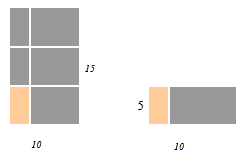
\includegraphics{get}
\caption{Copying Data from 2-dimensional 15x10 Global Array into Local Buffer 5x10 Array}
\label{get}
\end{figure}

Return: The local array buffer.

\end{desc}

\begin{pydesc}
If buffer is None, then a new ndarray will be allocated. Otherwise, the same
buffer that was passed in will be updated and returned.
\end{pydesc}

\apih{PERIODIC GET}{Get, with periodic boundary conditions, data from a global array}

\begin{capi}
\begin{ccode}
void NGA_Periodic_get(int g_a, int lo[], int hi[], void* buf, int ld[])
\end{ccode}
\begin{funcargs}
\inarg{int}{g_a}{global array handle}
\inarg{int}{ndim}{number of dimensions of the global array}
\inarg{int*}{lo[ndim]}{array of starting indices for global array section}
\inarg{int*}{hi[ndim]}{array of ending indices for global array section}
\outarg{void*}{buf}{pointer to the local buffer array where the data goes}
\inarg{int*}{ld[ndim-1]}{array specifying leading dimensions/strides/extents for buffer array}
\end{funcargs}
\end{capi}

\begin{fapi}
\begin{fcode}
subroutine nga_periodic_get(g_a, lo, hi,  buf, ld)
\end{fcode}
\begin{funcargs}
\inarg{integer}{g_a}{global array handle}
\inarg{integer}{ndim}{number of dimensions of the global array}
\inarg{integer}{lo(ndim)}{array of starting indices for global array section}
\inarg{integer}{hi(ndim)}{array of ending indices for global array section}
\outarg{type}{buf}{local buffer array where the data goes  to}
\inarg{integer}{ld(ndim-1)}{array specifying leading dimensions for buffer array}
\end{funcargs}
\end{fapi}

\begin{cxxapi}
\begin{cxxcode}
void GlobalArray::periodicGet(int lo[], int hi[], void* buf, int ld[]) const
void GlobalArray::periodicGet(int64_t lo[], int64_t hi[], void* buf,
								  int64_t ld[]) const
\end{cxxcode}
\begin{funcargs}
\inarg{int*}{lo[ndim]}{array of starting indices for global array section}
\inarg{int*}{hi[ndim]}{array of ending indices for global array section}
\outarg{void*}{buf}{pointer to the local buffer array where the data goes}
\inarg{int*}{ld[ndim-1]}{array specifying leading dimensions/strides/extents for buffer array}
\end{funcargs}
\end{cxxapi}

\begin{pyapi}
\begin{pycode}
ret = ga.periodic_get(int g_a, lo, hi, buffer, alpha=None)
\end{pycode}
\begin{funcargs}
\inarg{int}{g_a}{the array handle}
\inarg{1D array-like of ints}{lo}{lower bound patch coordinates, inclusive}
\inarg{1D array-like of ints}{hi}{higher bound patch coordinates, exclusive}
\inarg{ndarray}{buffer}{an ndarray of the appropriate type, large enough to hold lo,hi}
\outarg{ndarray}{ret}{local buffer array where the data goes to}
\end{funcargs}
\end{pyapi}

\ncoll

\begin{desc}

Same as nga_get except the indices can extend beyond the array
boundary/dimensions in which case the library wraps them around.

The local array is assumed to be have the same number of dimensions as the
global array. Any detected inconsitencies/errors in the input arguments are
fatal.

Returns: The local Array buffer.

\end{desc}

\seealso{GET}

\apih{STRIDED GET}{Get strided data from a global array }

\begin{capi}
\begin{ccode}
void NGA_Strided_get(int g_a, int lo[], int hi[], int skip[],
                     void* buf, int ld[])
\end{ccode}
\begin{funcargs}
\inarg{int}{g_a}{global array handle}
\inarg{int}{ndim}{number of dimensions of the global array}
\inarg{int*}{lo[ndim]}{array of starting indices for global array section}
\inarg{int*}{hi[ndim]}{array of ending indices for global array section}
\inarg{int*}{skip[ndim]}{array of strides for each dimension}
\outarg{void*}{buf}{pointer to the local buffer array where the data goes}
\inarg{int*}{ld[ndim-1]}{array specifying leading dimensions/strides/extents for buffer array}
\end{funcargs}
\end{capi}

\begin{fapi}
\begin{fcode}
subroutine nga_strided_get(g_a, lo, hi, skip, buf, ld)
\end{fcode}
\begin{funcargs}
\inarg{integer}{g_a}{global array handle}
\inarg{integer}{ndim}{number of dimensions of the global array}
\inarg{integer}{lo(ndim)}{array of starting indices for global array section}
\inarg{integer}{hi(ndim)}{array of ending indices for global array section}
\inarg{integer}{skip(ndim)}{array of strides for each dimension}
\outarg{type}{buf}{local buffer array where the data comes from}
\inarg{integer}{ld(ndim-1)}{array specifying leading dimensions for buffer array}
\end{funcargs}
\end{fapi}

\begin{cxxapi}
\begin{cxxcode}
void GlobalArray::stridedGet(int lo[], int hi[], int skip[],
                             void *buf, int ld[]) const
void GlobalArray::stridedGet(int64_t lo[], int64_t hi[], int64_t skip[],
                             void *buf, int64_t ld[]) const
\end{cxxcode}
\begin{funcargs}
\inarg{int*}{lo[ndim]}{array of starting indices for glob array section}
\inarg{int*}{hi[ndim]}{array of ending indices for global array section}
\inarg{int*}{skip[ndim]}{array of strides for each dimension}
\outarg{void*}{buf}{pointer to local buffer array where data goes}
\inarg{int*}{ld[ndim-1]}{array specifying leading dimensions/strides/extents for buffer array}
\end{funcargs}
\end{cxxapi}

\begin{pyapi}
\begin{pycode}
ret = ga.strided_get(int g_a, lo=None, hi=None, skip=None, ndarray buffer=None)
\end{pycode}
\begin{funcargs}
\inarg{int}{g_a}{the array handle}
\inarg{1D array-like of ints}{lo}{lower bound patch coordinates, inclusive}
\inarg{1D array-like of ints}{hi}{higher bound patch coordinates, exclusive}
\inarg{1D array-like of ints}{skip}{strides for each dimension}
\inarg{ndarray}{buffer}{an ndarray of the appropriate type, large enough to hold lo,hi}
\outarg{ndarray}{ret}{local buffer array where the data goes to}
\end{funcargs}
\end{pyapi}

\ncoll

\begin{desc}

This operation is the same as NGA_Get, except that the values corresponding to
dimension n in buf correspond to every skip[n] values of the global array g_a.

The local array is assumed to be have the same number of dimensions as the
global array. Any detected inconsitencies/errors in the input arguments are
fatal.

Returns: The local array buffer.

\end{desc}

\seealso{GET}

\apih{PUT}{Put data into a global array}

\begin{capi}
\begin{ccode}
void NGA_Put(int g_a, int lo[], int hi[], void* buf, int ld[])
\end{ccode}
\begin{funcargs}
\inarg{int}{g_a}{global array handle}
\inarg{int}{ndim}{number of dimensions of the global array}
\inarg{int*}{lo[ndim]}{array of starting indices for global array section}
\inarg{int*}{hi[ndim]}{array of ending indices for global array section}
\inarg{void*}{buf}{pointer to the local buffer array where the data is}
\inarg{int*}{ld[ndim-1]}{array specifying leading dimensions/strides/extents for buffer array}
\end{funcargs}
\end{capi}

\begin{f2dapi}
\begin{fcode}
subroutine ga_put(g_a, ilo, ihi, jlo, jhi, buf, ld)
\end{fcode}
\begin{funcargs}
\inarg{integer}{g_a}{}
\inarg{integer}{ilo, ihi, jlo, jhi}{}
\outarg{double precision/complex/integer}{buf}{TODO}
\inarg{integer}{ld}{}
\end{funcargs}
\end{f2dapi}

\begin{fapi}
\begin{fcode}
subroutine nga_put(g_a, lo, hi, buf, ld)
\end{fcode}
\begin{funcargs}
\inarg{integer}{g_a}{global array handle}
\inarg{integer}{ndim}{number of dimensions of the global array}
\inarg{integer}{lo(ndim)}{array of starting indices for global array section}
\inarg{integer}{hi(ndim)}{array of ending indices for global array section}
\outarg{type}{buf}{local buffer array where the data comes from}
\inarg{integer}{ld(ndim-1)}{array specifying leading dimensions for buffer array}
\end{funcargs}
\end{fapi}

\begin{cxxapi}
\begin{cxxcode}
void GlobalArray::put(int lo[], int hi[], void *buf, int ld[]) const
void GlobalArray::put(int64_t lo[], int64_t hi[], void *buf,
                      int64_t ld[]) const
\end{cxxcode}
\begin{funcargs}
\inarg{int*}{lo[ndim]}{array of starting indices for global array section}
\inarg{int*}{hi[ndim]}{array of ending indices for global array section}
\inarg{void*}{buf}{pointer to the local buffer array where the data is}
\inarg{int*}{ld[ndim-1]}{array specifying leading dimensions/strides/extents for buffer array}
\end{funcargs}
\end{cxxapi}

\begin{pyapi}
\begin{pycode}
ga.put(int g_a, buffer, lo=None, hi=None)
\end{pycode}
\begin{funcargs}
\inarg{int}{g_a}{the array handle}
\inarg{array-like}{buffer}{the data to put}
\inarg{1D array-like of ints}{lo}{lower bound patch coordinates, inclusive}
\inarg{1D array-like of ints}{hi}{higher bound patch coordinates, exclusive}
\end{funcargs}
\end{pyapi}

\ncoll

\begin{desc}

Copies data from the local array buffer to the global array section. The local
array is assumed to have the same number of dimensions as the global array.
Any detected inconsistencies or errors in input arguments are fatal.

\end{desc}

\apih{PERIODIC PUT}{Put, with periodic boundary conditions, data into a global array}

\begin{capi}
\begin{ccode}
void NGA_Periodic_put(int g_a, int lo[], int hi[], void* buf, int ld[])
\end{ccode}
\begin{funcargs}
\inarg{int}{g_a}{global array handle}
\inarg{int}{ndim}{number of dimensions of the global array}
\inarg{int*}{lo[ndim]}{array of starting indices for global array section}
\inarg{int*}{hi[ndim]}{array of ending indices for global array section}
\inarg{void*}{buf}{pointer to the local buffer array where the data is}
\inarg{int*}{ld[ndim-1]}{array specifying leading dimensions/strides/extents for buffer array}
\end{funcargs}
\end{capi}

\begin{fapi}
\begin{fcode}
subroutine nga_periodic_put(g_a, lo, hi,  buf, ld)
\end{fcode}
\begin{funcargs}
\inarg{integer}{g_a}{global array handle}
\inarg{integer}{ndim}{number of dimensions of the global array}
\inarg{integer}{lo(ndim)}{array of starting indices for global array section}
\inarg{integer}{hi(ndim)}{array of ending indices for global array section}
\outarg{type}{buf}{local buffer array where the data comes from}
\inarg{integer}{ld(ndim-1)}{array specifying leading dimensions for buffer array}
\end{funcargs}
\end{fapi}

\begin{cxxapi}
\begin{cxxcode}
void GlobalArray::periodicPut(int lo[], int hi[], void* buf, int ld[]) const
void GlobalArray::periodicPut(int64_t lo[], int64_t hi[], void* buf, int64_t ld[]) const
\end{cxxcode}
\begin{funcargs}
\inarg{int*}{lo[ndim]}{array of starting indices for global array section}
\inarg{int*}{hi[ndim]}{array of ending indices for global array section}
\inarg{void*}{buf}{pointer to the local buffer array where the data goes}
\inarg{int*}{ld[ndim-1]}{array specifying leading dimensions/strides/extents for buffer array}
\end{funcargs}
\end{cxxapi}

\begin{pyapi}
\begin{pycode}
ga.periodic_put(int g_a, buffer, lo=None, hi=None)
\end{pycode}
\begin{funcargs}
\inarg{int}{g_a}{the array handle}
\inarg{array-like}{buffer}{the data to put}
\inarg{1D array-like of ints}{lo}{lower bound patch coordinates, inclusive}
\inarg{1D array-like of ints}{hi}{higher bound patch coordinates, exclusive}
\end{funcargs}
\end{pyapi}

\ncoll

\begin{desc}

Same as nga_put except the indices can extend beyond the array
boundary/dimensions in which case the library wraps them around.  The indices
can extend beyond the array boundary/dimensions in which case the libray wraps
them around.  Copies data from local array buffer to the global array section.
The local array is assumed to be have the same number of dimensions as the
global array. Any detected inconsitencies/errors in input arguments are fatal.

\end{desc}

\seealso{PUT}

\apih{STRIDED PUT}{Put strided data into a global array}

\begin{capi}
\begin{ccode}
void NGA_Strided_put(int g_a, int lo[], int hi[], int skip[],
                     void* buf, int ld[])
\end{ccode}
\begin{funcargs}
\inarg{}{g_a}{global array handle}
\inarg{}{ndim}{number of dimensions of the global array}
\inarg{}{lo[ndim]}{array of starting indices for global array section}
\inarg{}{hi[ndim]}{array of ending indices for global array section}
\inarg{}{skip[ndim]}{array of strides for each dimension}
\outarg{}{buf}{pointer to the local buffer array where the data goes}
\inarg{}{ld[ndim-1]}{array specifying leading dimensions/strides/extents for buffer array}
\end{funcargs}
\end{capi}

\begin{fapi}
\begin{fcode}
subroutine nga_strided_put(g_a, lo, hi, skip, buf, ld)
\end{fcode}
\begin{funcargs}
\inarg{integer}{g_a}{global array handle}
\inarg{integer}{ndim}{number of dimensions of the global array}
\inarg{integer}{lo(ndim)}{array of starting indices for global}
\inarg{integer}{hi(ndim)}{array of ending indices for global array}
\inarg{integer}{skip(ndim)}{array of strides for each dimension}
\outarg{type}{buf}{local buffer array where the data comes from}
\inarg{integer}{ld(ndim-1)}{array specifying leading dimensions for array section}
\end{funcargs}
\end{fapi}

\begin{cxxapi}
\begin{cxxcode}
void GlobalArray::stridedPut(int lo[], int hi[], int skip[],
                             void*buf, int ld[]) const
void GlobalArray::stridedPut(int64_t lo[], int64_t hi[], int64_t skip[],
                             void *buf, int64_t ld[]) const
\end{cxxcode}
\begin{funcargs}
\inarg{int*}{lo[ndim]}{array of starting indices for glob array section}
\inarg{int*}{hi[ndim]}{array of ending indices for global array section}
\inarg{int*}{skip[ndim]}{array of strides for each dimension}
\inarg{void*}{buf}{pointer to local buffer array where data goes}
\inarg{int*}{ld[ndim-1]}{array specifying leading dimensions/strides/extents for buffer array}
\end{funcargs}
\end{cxxapi}

\begin{pyapi}
\begin{pycode}
ga.strided_put(int g_a, buffer, lo=None, hi=None, skip=None)
\end{pycode}
\begin{funcargs}
\inarg{int}{g_a}{the array handle}
\inarg{array-like}{buffer}{the data to put}
\inarg{1D array-like of ints}{lo}{lower bound patch coordinates, inclusive}
\inarg{1D array-like of ints}{hi}{higher bound patch coordinates, exclusive}
\end{funcargs}
\end{pyapi}

\ncoll

\begin{desc}

Strided version of put.  This operation is the same as NGA_Put, except that the
values corresponding to dimension n in buf are copied to every skip[n] values
of the global array g_a.

Copies data from local array buffer to the global array section.

The local array is assumed to be have the same number of dimensions as the
global array.

Any detected inconsitencies/errors in input arguments are fatal.

\end{desc}

\seealso{PUT}

\apih{ACC}{Accumulate data into a global array}

\begin{capi}
\begin{ccode}
void NGA_Acc(int g_a, int lo[], int hi[], void* buf, int ld[],
             void* alpha)
\end{ccode}
\begin{funcargs}
\inarg{int}{g_a}{global array handle}
\inarg{int}{ndim}{number of dimensions of the global array}
\inarg{int*}{lo[ndim]}{array of starting indices for array section}
\inarg{int*}{hi[ndim]}{array of ending indices for array section}
\inarg{void*}{buf}{pointer to the local buffer array}
\inarg{int*}{ld[ndim-1]}{array specifying leading dimensions/strides/extents for buffer array}
\inarg{double/double complex/long*}{alpha}{scale factor}
\end{funcargs}
\end{capi}

\begin{f2dapi}
\begin{fcode}
subroutine ga_acc(g_a, ilo, ihi, jlo, jhi, buf, ld, alpha)
\end{fcode}
\begin{funcargs}
\inarg{integer}{g_a}{}
\inarg{integer}{ilo, ihi, jlo, jhi}{}
\inarg{double precision/complex}{buf}{TODO}
\inarg{integer}{ld}{}
\inarg{double precision/complex}{alpha}{TODO}
\end{funcargs}
\end{f2dapi}

\begin{fapi}
\begin{fcode}
subroutine nga_acc(g_a, lo, hi, buf, ld, alpha)
\end{fcode}
\begin{funcargs}
\inarg{integer}{g_a}{global array handle}
\inarg{integer}{ndim}{number of dimensions of the global array}
\inarg{integer}{lo(ndim)}{array of starting indices for global array section}
\inarg{integer}{hi(ndim)}{array of ending indices for global array section}
\outarg{type}{buf}{local buffer array where the local data is}
\inarg{integer}{ld(ndim-1)}{array specifying leading dimensions for buffer array}
\inarg{type}{alpha}{scale argument for accumulate}
\end{funcargs}
\end{fapi}

\begin{cxxapi}
\begin{cxxcode}
void GlobalArray::acc(int lo[], int hi[], void *buf,
                      int ld[], void *alpha) const
void GlobalArray::acc(int64_t lo[], int64_t hi[], void *buf,
                      int64_t ld[], void *alpha) const
\end{cxxcode}
\begin{funcargs}
\inarg{int*}{lo[ndim]}{array of starting indices for array section}
\inarg{int*}{hi[ndim]}{array of ending indices for array section}
\inarg{void*}{buf}{pointer to the local buffer array}
\inarg{int*}{ld[ndim-1]}{array specifying leading dimensions/strides/extents for buffer array}
\inarg{void*}{alpha}{scale factor (double/double complex/long *)}
\end{funcargs}
\end{cxxapi}

\begin{pyapi}
\begin{pycode}
ga.acc(int g_a, buffer, lo=None, hi=None, alpha=None)
\end{pycode}
\begin{funcargs}
\inarg{int}{g_a}{the array handle}
\inarg{array-like}{buffer}{the data to put}
\inarg{1D array-like of ints}{lo}{lower bound patch coordinates, inclusive}
\inarg{1D array-like of ints}{hi}{higher bound patch coordinates, exclusive}
\inarg{object}{alpha}{scale factor, cast to the appropriate type}
\end{funcargs}
\end{pyapi}

\ncoll

\begin{desc}

Combines data from local array buffer with data in the global array section.
The local array is assumed to be have the same number of dimensions as the
global array.

global array section (lo[],hi[]) += *alpha * buffer

\end{desc}

\apih{PERIODIC ACC}{Accumulate, with periodic boundary conditions, data into a global array}

\begin{capi}
\begin{ccode}
void NGA_Periodic_acc(int g_a, int lo[], int hi[], void* buf, int ld[],
                      void* alpha)
\end{ccode}
\begin{funcargs}
\inarg{int}{g_a}{global array handle}
\inarg{int}{ndim}{number of dimensions of the global array}
\inarg{int*}{lo[ndim]}{array of starting indices for array section}
\inarg{int*}{hi[ndim]}{array of ending indices for array section}
\inarg{void*}{buf}{pointer to the local buffer array}
\inarg{int*}{ld[ndim-1]}{array specifying leading dimensions/strides/extents for buffer array}
\inarg{double/double complex/long*}{alpha}{scale factor}
\end{funcargs}
\end{capi}

\begin{fapi}
\begin{fcode}
subroutine nga_periodic_acc(g_a, lo, hi, buf, ld, alpha)
\end{fcode}
\begin{funcargs}
\inarg{integer}{g_a}{global array handle}
\inarg{integer}{ndim}{number of dimensions of the global array}
\inarg{integer}{lo(ndim)}{array of starting indices for global array section}
\inarg{integer}{hi(ndim)}{array of ending indices for global array section}
\outarg{type}{buf}{local buffer array where the local data is}
\inarg{integer}{ld(ndim-1)}{array specifying leading dimensions for buffer array}
\inarg{type}{alpha}{scale argument for accumulate}
\end{funcargs}
\end{fapi}

\begin{cxxapi}
\begin{cxxcode}
void GlobalArray::periodicAcc(int lo[], int hi[], void* buf,
                              int ld[], void* alpha) const
void GlobalArray::periodicAcc(int64_t lo[], int64_t hi[], void* buf,
                              int64_t ld[], void* alpha) const
\end{cxxcode}
\begin{funcargs}
\inarg{int*}{lo[ndim]}{array of starting indices for array section}
\inarg{int*}{hi[ndim]}{array of ending indices for array section}
\inarg{void*}{buf}{pointer to the local buffer array}
\inarg{int*}{ld[ndim-1]}{array specifying leading dimensions/strides/extents for buffer array}
\inarg{}{alpha}{double/double complex/long scale factor}
\end{funcargs}
\end{cxxapi}

\begin{pyapi}
\begin{pycode}
ga.periodic_acc(int g_a, buffer, lo=None, hi=None, alpha=None)
\end{pycode}
\begin{funcargs}
\inarg{int}{g_a}{the array handle}
\inarg{array-like}{buffer}{the data to put}
\inarg{1D array-like of ints}{lo}{lower bound patch coordinates, inclusive}
\inarg{1D array-like of ints}{hi}{higher bound patch coordinates, exclusive}
\inarg{object}{alpha}{scale factor, cast to the appropriate type}
\end{funcargs}
\end{pyapi}

\ncoll

\begin{desc}

Same as nga_acc except the indices can extend beyond the array
boundary/dimensions in which case the library wraps them around. For Python,
this is the periodic version of ga.acc.

Combines data from buffer with data in the global array patch.

The buffer array is assumed to be have the same number of dimensions as the
global array. If the buffer is not contiguous, a contiguous copy will be made.

global array section (lo[],hi[]) += alpha * buffer

\end{desc}

\seealso{ACC}

\apih{STRIDED ACC}{Accumulate strided data into a global array}

\begin{capi}
\begin{ccode}
void NGA_Strided_acc(int g_a, int lo[], int hi[], int skip[], void* buf,
                     int ld[])
\end{ccode}
\begin{funcargs}
\inarg{int}{g_a}{global array handle}
\inarg{int}{ndim}{number of dimensions of the global array}
\inarg{int*}{lo[ndim]}{array of starting indices for global array section}
\inarg{int*}{hi[ndim]}{array of ending indices for global array section}
\inarg{int*}{skip[ndim]}{array of strides for each dimension}
\inarg{void*}{buf}{pointer to the local buffer array where the data goes}
\inarg{int*}{ld[ndim-1]}{array specifying leading dimensions/strides/extents for buffer array}
\inarg{double/DoubleComplex/long*}{alpha}{scale factor}
\end{funcargs}
\end{capi}

\begin{fapi}
\begin{fcode}
subroutine nga_strided_acc(g_a, lo, hi, skip, buf, ld, alpha)
\end{fcode}
\begin{funcargs}
\inarg{integer}{g_a}{global array handle}
\inarg{integer}{ndim}{number of dimensions of the global array}
\inarg{integer}{lo(ndim)}{array of starting indices for global array section}
\inarg{integer}{hi(ndim)}{array of ending indices for global array section}
\inarg{integer}{skip(ndim)}{array of strides for each dimension}
\inarg{type}{buf}{local buffer array where the data comes from}
\inarg{integer}{ld(ndim-1)}{array specifying leading dimensions for buffer array}
\inarg{type}{alpha}{scale argument for accumulate}
\end{funcargs}
\end{fapi}

\begin{cxxapi}
\begin{cxxcode}
void GlobalArray::stridedAcc(int lo[], int hi[], int skip[], void *buf,
                             int ld[], void *alpha) const;
void GlobalArray::stridedAcc(int64_t lo[], int64_t hi[], int64_t skip[],
                             void *buf, int64_t ld[], void *alpha) const;
\end{cxxcode}
\begin{funcargs}
\inarg{int*}{lo[ndim]}{array of starting indices for glob array section}
\inarg{int*}{hi[ndim]}{array of ending indices for global array section}
\inarg{int*}{skip[ndim]}{array of strides for each dimension}
\inarg{void*}{buf}{pointer to local buffer array where data goes}
\inarg{int*}{ld[ndim-1]}{array specifying leading dimensions/strides/extents for buffer array}
\inarg{void*}{alpha}{double/DoubleComplex/long scale factor}
\end{funcargs}
\end{cxxapi}

\begin{pyapi}
\begin{pycode}
ga.strided_acc(int g_a, buffer, lo=None, hi=None, skip=None, alpha=None)
\end{pycode}
\begin{funcargs}
\inarg{int}{g_a}{the array handle}
\inarg{array-like}{buffer}{the data to put}
\inarg{1D array-like of ints}{lo}{lower bound patch coordinates, inclusive}
\inarg{1D array-like of ints}{hi}{higher bound patch coordinates, exclusive}
\inarg{1D array-like of ints}{skip}{strides for each dimension}
\inarg{object}{alpha}{scale factor, cast to the appropriate type}
\end{funcargs}
\end{pyapi}

\ncoll

\begin{desc}

This operation is the same as NGA_Acc, except that the values corresponding to
dimension n in buf are accumulated to every skip[n] values of the global array
g_a.

Combines data from buffer with data in the global array patch.

The buffer array is assumed to be have the same number of dimensions as the
global array.

global array section (lo[],hi[]) += alpha * buffer

\end{desc}

\seealso{ACC}

\apih{DISTRIBUTION}{Inquire data range on a specified processor}

\begin{capi}
\begin{ccode}
void NGA_Distribution(int g_a, int iproc, int lo[], int hi[])
\end{ccode}
\begin{funcargs}
\inarg{int}{g_a}{array handle}
\inarg{int}{iproc}{process number}
\inarg{int}{ndim}{number of dimensions of the global array}
\outarg{int*}{lo[ndim]}{array of starting indices for array section}
\outarg{int*}{hi[ndim]}{array of ending indices for array section}
\end{funcargs}
\end{capi}

\begin{f2dapi}
\begin{fcode}
subroutine ga_distribution(g_a, iproc, ilo, ihi, jlo, jhi)
\end{fcode}
\begin{funcargs}
\inarg{integer}{g_a}{array handle}
\inarg{integer}{iproc}{process number}
\outarg{integer}{ilo,ihi,jlo,jhi}{range held by process iproc}
\end{funcargs}
\end{f2dapi}

\begin{fapi}
\begin{fcode}
subroutine nga_distribution(g_a, iproc, lo, hi)
\end{fcode}
\begin{funcargs}
\inarg{integer}{g_a}{array handle}
\inarg{integer}{iproc}{process number}
\inarg{integer}{ndim}{number of dimensions}
\outarg{integer}{lo(ndim),hi(ndim)}{range held by process iproc}
\end{funcargs}
\end{fapi}

\begin{cxxapi}
\begin{cxxcode}
void GlobalArray::distribution(int me, int* lo, int* hi) const
void GlobalArray::distribution(int me, int64_t* lo, int64_t* hi) const
\end{cxxcode}
\begin{funcargs}
\inarg{int}{iproc}{process number}
\outarg{int*}{lo[ndim]}{array of starting indices for array section}
\outarg{int*}{hi[ndim]}{array of ending indices for array section}
\end{funcargs}
\end{cxxapi}

\begin{pyapi}
\begin{pycode}
lo,hi = ga.distribution(int g_a, int iproc=-1)
\end{pycode}
\begin{funcargs}
\inarg{int}{g_a}{array handle}
\inarg{int}{iproc}{process number}
\outarg{1D ndarray of ints}{lo}{array of starting indices for array section}
\outarg{1D ndarray of ints}{hi}{array of ending indices for array section}
\end{funcargs}
\end{pyapi}

\local

\begin{desc}

If no array elements are owned by process iproc, the range is returned as
lo[ ]=0 and hi[ ]= -1 for all dimensions.

Return the distribution given to iproc. If iproc is not specified, then
ga.nodeid() is used. The range is returned as -1 for lo and -2 for hi if no
elements are owned by iproc.

\end{desc}

\apih{COMPARE DISTR}{Compare distribution of two global arrays}

\begin{capi}
\begin{ccode}
int GA_Compare_distr(int g_a, int g_b)
\end{ccode}
\begin{funcargs}
\inarg{int}{g_a, g_b}{array handles}
\outarg{int}{}{0 if distributions are identical}
\end{funcargs}
\end{capi}

\begin{fapi}
\begin{fcode}
logical function ga_compare_distr(g_a, g_b)
\end{fcode}
\begin{funcargs}
\inarg{integer}{g_a, g_b}{array handles}
\outarg{logical}{}{.TRUE. if distributions are identical}
\end{funcargs}
\end{fapi}

\begin{cxxapi}
\begin{cxxcode}
int GlobalArray::compareDistr(const GlobalArray *g_a) const
\end{cxxcode}
\begin{funcargs}
\inarg{int}{g_a}{GlobalArray to compare against}
\outarg{int}{}{0 if distributions are identical}
\end{funcargs}
\end{cxxapi}

\begin{pyapi}
\begin{pycode}
ret = ga.compare_distr(int g_a, int g_b)
\end{pycode}
\begin{funcargs}
\inarg{int}{g_a}{array handle}
\inarg{int}{g_b}{array handle}
\outarg{bool}{ret}{True if distributions are identical}
\end{funcargs}
\end{pyapi}

\gcoll

\begin{desc}

Compares distributions of two global arrays. Returns 0 if distributions are
identical and 1 when they are not.

\end{desc}

\apih{ACCESS}{Access data locally allocated for a global array}

\begin{capi}
\begin{ccode}
void NGA_Access(int g_a, int lo[], int hi[], void *ptr, int ld[])
\end{ccode}
\begin{funcargs}
\inarg{int}{g_a}{global array handle}
\inarg{int}{ndim}{number of dimensions of the global array}
\inarg{int*}{lo[ndim]}{array of starting indices for array section}
\inarg{int*}{hi[ndim]}{array of ending indices for array section}
\outarg{void**}{ptr}{points to location of first element in patch}
\outarg{int*}{ld[ndim-1]}{leading dimensions for the pacth elements}
\end{funcargs}
\end{capi}

\begin{f2dapi}
\begin{fcode}
subroutine ga_access(g_a, ilo, ihi, jlo, jhi, index, ld)
\end{fcode}
\begin{funcargs}
\inarg{integer}{g_a}{}
\inarg{integer}{ilo, ihi, jlo, jhi}{}
\outarg{integer}{index}{}
\outarg{integer}{ld}{}
\end{funcargs}
\end{f2dapi}

\begin{fapi}
\begin{fcode}
subroutine nga_access(g_a, lo, hi, index, ld)
\end{fcode}
\begin{funcargs}
\inarg{integer}{g_a}{array handle}
\inarg{integer}{ndim}{number of array dimensions}
\inarg{integer}{lo(ndim),hi(ndim)}{patch specification}
\outarg{integer}{index}{reference to local data}
\outarg{integer}{ld(ndim-1)}{array of leading dimensions}
\end{funcargs}
\end{fapi}

\begin{cxxapi}
\begin{cxxcode}
void GlobalArray::access(int lo[], int hi[], void *ptr, int ld[]) const
void GlobalArray::access(int64_t lo[], int64_t hi[], void *ptr, int64_t ld[]) cons
\end{cxxcode}
\begin{funcargs}
\inarg{int*}{lo[ndim]}{array of starting indices for array section}
\inarg{int*}{hi[ndim]}{array of ending indices for array section}
\outarg{void**}{ptr}{points to location of first element in patch}
\outarg{int*}{ld[ndim-1]}{leading dimensions for the pacth elements}
\end{funcargs}
\end{cxxapi}

\begin{pyapi}
\begin{pycode}
ret = ga.access(int g_a, lo=None, hi=None)
\end{pycode}
\begin{funcargs}
\inarg{int}{g_a}{the array handle}
\inarg{1D array-like of ints}{lo}{lower bound patch coordinates, inclusive}
\inarg{1D array-like of ints}{hi}{higher bound patch coordinates, exclusive}
\end{funcargs}
\end{pyapi}

\local

\begin{desc}

Provides access to the specified patch of a global array. Returns array of
leading dimensions ld and a pointer to the first element in the patch.  This
routine allows to access directly, in place elements in the local section of a
global array. It useful for writing new GA operations. A call to ga_access
normally follows a previous call to ga_distribution that returns coordinates of
the patch associated with a processor. You need to make sure that the
coordinates of the patch are valid (test values returned from ga_distribution).

Each call to ga_access has to be followed by a call to either ga_release or
ga_release_update. You can access in this fashion only local data.  Since the
data is shared with other processes, you need to consider issues of mutual
exclusion.

\end{desc}

\begin{pydesc}
Note: The entire local data is always accessed, but if a smaller patch is
requested, an appropriately sliced ndarray is returned.
\end{pydesc}

\begin{fdesc}

Provides access to the specified patch of array. Returns leading dimension ld
and and MA-like index for the data. This routine is intended for writing new GA
operations. Call to ga_access should normally follow a call to ga_distribution
that returns coordinates of the patch associated with a processor. You need to
make sure that the coordinates of the patch are valid (test values returned
from ga_distribution).

Your code should include a MA include file, mafdecls.h.
\begin{verbatim}
          dbl_mb(index)  - for double precision data
          int_mb(index)  - for integer data
          dcpl_mb(index) - for double complex data
\end{verbatim}

The addressing convention refers the first element (ilo,jlo) of the patch.
However, you can only pass that reference to another subroutine where it could
be used like a normal array, see the following example. This constraint caused
by the HP fortran compiler inability to reference shared memory data properly.
The C interface has no such restrictions.

Example

For a given subroutine:
\begin{verbatim}
          subroutine foo(A,  nrows, ncols lda)
          double precision A(lda,*)
          integer nrows, ncols
             ....
          end
\end{verbatim}
you can reference A(ilo:ihi,jlo:jhi) in the following way:

\begin{verbatim}
          call foo(dbl_mb(index), ihi-ilo+1, jhi-jlo+1, lda)
\end{verbatim}

\end{fdesc}


\apih{ACCESS BLOCK SEGMENT}{Access local data for a specific global array block}

\begin{capi}
\begin{ccode}
void NGA_Access_block_segment(int g_a, int proc, void *ptr, int *len)
\end{ccode}
\begin{funcargs}
\inarg{int}{g_a}{array handle}
\inarg{int}{proc}{processor ID}
\outarg{void**}{ptr}{pointer to locally held data}
\outarg{int*}{len}{length of data on processor}
\end{funcargs}
\end{capi}

\begin{fapi}
\begin{fcode}
subroutine nga_access_block_segment(g_a, proc, index, len)
\end{fcode}
\begin{funcargs}
\inarg{integer}{g_a}{array handle}
\inarg{integer}{proc}{processor ID}
\outarg{integer}{index}{reference to local data}
\outarg{integer}{len}{length of data on processor}
\end{funcargs}
\end{fapi}

\begin{cxxapi}
\begin{cxxcode}
void GlobalArray::accessBlockSegment(int index, void *ptr,
                                     int *len) const
void GlobalArray::accessBlockSegment(int index, void *ptr,
                                     int64_t *len) const
\end{cxxcode}
\begin{funcargs}
\inarg{int}{index}{processor ID}
\outarg{void**}{ptr}{points to location of first element}
\outarg{int*}{len}{length of locally held data}
\end{funcargs}
\end{cxxapi}

\begin{pyapi}
\begin{pycode}
ret = ga.access_block(int g_a, int proc)
\end{pycode}
\begin{funcargs}
\inarg{int}{g_a}{array handle}
\inarg{int}{proc}{processor ID}
\outarg{ndarray}{ret}{locally held data}
\end{funcargs}
\end{pyapi}

\local

\begin{desc}

This function can be used to gain access to the all the locally held data on a
particular processor that is associated with a block-cyclic distributed array.
Once the index has been returned, local data can be accessed as described in
the documentation for NGA_Access. The parameter len is the number of data
elements that are held locally. The data inside this segment has a lot of
additional structure so this function is not generally useful to developers. It
is primarily used inside the GA library to implement other GA routines. Each
call to ga_access_block_segment should be followed by a call to either
NGA_Release_block_segment or NGA_Release_update_block_segment.

\end{desc}

\seealso{ACCESS,RELEASE BLOCK SEGMENT,RELEASE UPDATE BLOCK SEGMENT}

\apih{ACCESS BLOCK}{Access a block in a block-cyclic distributed global array}

\begin{capi}
\begin{ccode}
void NGA_Access_block(int g_a, int idx, void *ptr, int ld[])
\end{ccode}
\begin{funcargs}
\inarg{int}{g_a}{array handle}
\inarg{int}{ndim}{number of array dimensions}
\inarg{int}{idx}{block index}
\outarg{void**}{ptr}{pointer to locally held block}
\outarg{int*}{ld[ndim-1]}{array of leading dimensions}
\end{funcargs}
\end{capi}

\begin{fapi}
\begin{fcode}
subroutine nga_access_block(g_a, idx, index, ld)
\end{fcode}
\begin{funcargs}
\inarg{integer}{g_a}{array handle}
\inarg{integer}{ndim}{number of array dimensions}
\inarg{integer}{idx}{block index}
\outarg{integer}{index}{reference to local data}
\outarg{integer}{ld(ndim-1)}{array of leading dimensions}
\end{funcargs}
\end{fapi}

\begin{cxxapi}
\begin{cxxcode}
void GlobalArray::accessBlock(int idx, void *ptr, int ld[]) const
void GlobalArray::accessBlock(int64_t idx, void *ptr, int64_t ld[]) const
\end{cxxcode}
\begin{funcargs}
\inarg{int}{idx}{index of block}
\outarg{void**}{ptr}{points to location of first element in patch}
\outarg{int*}{ld[ndim-1]}{leading dimensions for the pacth elements}
\end{funcargs}
\end{cxxapi}

\begin{pyapi}
\begin{pycode}
ret = ga.access_block_grid(int g_a, int idx)
\end{pycode}
\begin{funcargs}
\inarg{int}{g_a}{array handle}
\inarg{int}{idx}{block index}
\outarg{ndarray}{ret}{array representing the block at index idx}
\end{funcargs}
\end{pyapi}

\local

\begin{desc}

This function can be used to gain direct access to the data represented by a
single block in a global array with a block-cyclic data distribution.  The
index idx is the index of the block in the array assuming that blocks are
numbered sequentially in a column-major order. A quick way of determining
whether a block with index idx is held locally on a processor is to calculate
whether mod(idx,nproc) equals the processor ID, where nproc is the total number
of processors. Once the index has been returned, local data can be accessed as
described in the documentation for NGA_Access. Each call to ga_access_block
should be followed by a call to either NGA_Release_block or
NGA_Release_update_block.

\end{desc}

\seealso{ACCESS,RELEASE BLOCK,RELEASE UPDATE BLOCK}

\apih{ACCESS BLOCK GRID}{Access data block in a block-cyclic distributed global array}

\begin{capi}
\begin{ccode}
void NGA_Access_block_grid(int g_a, int subscript[], void *ptr, int ld[])
\end{ccode}
\begin{funcargs}
\inarg{int}{g_a}{array handle}
\inarg{int}{ndim}{number of array dimensions}
\inarg{int*}{subscript[ndim]}{subscript of block in array}
\outarg{void**}{ptr}{pointer to locally held bloc}
\outarg{int*}{ld[ndim-1]}{array of leading dimensions}
\end{funcargs}
\end{capi}

\begin{fapi}
\begin{fcode}
subroutine nga_access_block_grid(g_a, subscript, index, ld)
\end{fcode}
\begin{funcargs}
\inarg{integer}{g_a}{array handle}
\inarg{integer}{ndim}{number of array dimensions}
\inarg{integer}{subscript(ndim)}{subscript of block in array}
\outarg{integer}{index}{reference to local data}
\outarg{integer}{ld(ndim-1)}{array of leading dimensions}
\end{funcargs}
\end{fapi}

\begin{cxxapi}
\begin{cxxcode}
void GlobalArray::accessBlockGrid(int index[], void *ptr, int ld[]) const
void GlobalArray::accessBlockGrid(int64_t index[], void *ptr, int64_t ld[])
                                  const
\end{cxxcode}
\begin{funcargs}
\inarg{int*}{index[ndim]}{indices of block in processor grid}
\outarg{void**}{ptr}{points to location of first element in patch}
\outarg{int*}{ld[ndim-1]}{leading dimensions for the pacth elements}
\end{funcargs}
\end{cxxapi}

\begin{pyapi}
\begin{pycode}
ret = ga.access_block_grid(int g_a, subscript)
\end{pycode}
\begin{funcargs}
\inarg{int}{g_a}{array handle}
\inarg{1D array-like of ints}{subscript}{subscript of block in array}
\outarg{void**}{ret}{pointer to locally held bloc}
\end{funcargs}
\end{pyapi}

\local

\begin{desc}

This function can be used to gain direct access to the data represented by a
single block in a global array with a SCALAPACK block-cyclic data distribution
that is based on an underlying processor grid. The subscript array contains the
subscript of the block in the array of blocks. This subscript is based on the
location of the block in a grid, each of whose dimensions is equal to the
number of blocks that fit along that dimension. Once the index has been
returned, local data can be accessed as described in the documentation for
NGA_Access. Each call to ga_access_block_grid should be followed by a call to
either NGA_Release_block_grid or NGA_Release_update_block_grid.

Returns: ndarray representing local block

\end{desc}

\seealso{ACCESS,RELEASE BLOCK GRID,RELEASE UPDATE BLOCK GRID}

\apih{RELEASE}{Release access to a global array}

\begin{capi}
\begin{ccode}
void NGA_Release(int g_a, int lo[], int hi[])
\end{ccode}
\begin{funcargs}
\inarg{int}{g_a}{global array handle}
\inarg{int}{ndim}{number of dimensions of the global array}
\inarg{int*}{lo[ndim]}{array of starting indices for array section}
\inarg{int*}{hi[ndim]}{array of ending indices for array section}
\end{funcargs}
\end{capi}

\begin{f2dapi}
\begin{fcode}
subroutine ga_release(g_a, ilo, ihi, jlo, jhi)
\end{fcode}
\begin{funcargs}
\inarg{integer}{g_a}{}
\inarg{integer}{ilo, ihi, jlo, jhi}{}
\end{funcargs}
\end{f2dapi}

\begin{fapi}
\begin{fcode}
subroutine nga_release(g_a, lo, hi)
\end{fcode}
\begin{funcargs}
\inarg{integer}{g_a}{array handle}
\inarg{integer}{ndim}{number of array dimensions}
\inarg{integer}{lo(ndim),hi(ndim)}{patch specification}
\end{funcargs}
\end{fapi}

\begin{cxxapi}
\begin{cxxcode}
void GlobalArray::release(int lo[], int hi[]) const
void GlobalArray::release(int64_t lo[], int64_t hi[]) const
\end{cxxcode}
\begin{funcargs}
\inarg{int*}{lo[ndim]}{array of starting indices for array section}
\inarg{int*}{hi[ndim]}{array of ending indices for array section}
\end{funcargs}
\end{cxxapi}

\begin{pyapi}
\begin{pycode}
ga.release(int g_a, lo=None, hi=None)
\end{pycode}
\begin{funcargs}
\inarg{int}{g_a}{the array handle}
\inarg{1D array-like of ints}{lo}{lower bound patch coordinates, inclusive}
\inarg{1D array-like of ints}{hi}{higher bound patch coordinates, exclusive}
\end{funcargs}
\end{pyapi}

\local

\begin{desc}

Releases access to a global array when the data was read only.

Your code should look like:
\begin{verbatim}
        NGA_Distribution(g_a, myproc, lo,hi);
        NGA_Access(g_a, lo, hi, \&ptr, ld);

             <operate on the data referenced by ptr>
        GA_Release(g_a, lo, hi);
\end{verbatim}
NOTE: see restrictions specified for ga_access.

\end{desc}

\seealso{ACCESS}

\apih{RELEASE UPDATE}{Release access to a global array after an update}

\begin{capi}
\begin{ccode}
void NGA_Release_update(int g_a, int lo[], int hi[])
\end{ccode}
\begin{funcargs}
\inarg{int}{g_a}{global array handle}
\inarg{int}{ndim}{number of dimensions of the global array}
\inarg{int*}{lo[ndim]}{array of starting indices for array section}
\inarg{int*}{hi[ndim]}{array of ending indices for array section}
\end{funcargs}
\end{capi}

\begin{f2dapi}
\begin{fcode}
subroutine ga_release_update(g_a, ilo, ihi, jlo, jhi)
\end{fcode}
\begin{funcargs}
\inarg{integer}{g_a}{}
\inarg{integer}{ilo, ihi, jlo, jhi}{}
\end{funcargs}
\end{f2dapi}

\begin{fapi}
\begin{fcode}
subroutine nga_release_update(g_a, lo, hi)
\end{fcode}
\begin{funcargs}
\inarg{integer}{g_a}{array handle}
\inarg{integer}{ndim}{number of array dimensions}
\inarg{integer}{lo(ndim),hi(ndim)}{patch specification}
\end{funcargs}
\end{fapi}

\begin{cxxapi}
\begin{cxxcode}
void GlobalArray::releaseUpdate(int lo[], int hi[]) const
void GlobalArray::releaseUpdate(int64_t lo[], int64_t hi[]) const
\end{cxxcode}
\begin{funcargs}
\inarg{int*}{lo[ndim]}{array of starting indices for array section}
\inarg{int*}{hi[ndim]}{array of ending indices for array section}
\end{funcargs}
\end{cxxapi}

\begin{pyapi}
\begin{pycode}
ga.release_update(int g_a, lo=None, hi=None)
\end{pycode}
\begin{funcargs}
\inarg{int}{g_a}{the array handle}
\inarg{1D array-like of ints}{lo}{lower bound patch coordinates, inclusive}
\inarg{1D array-like of ints}{hi}{higher bound patch coordinates, exclusive}
\end{funcargs}
\end{pyapi}

\local

\begin{desc}

Releases access to the data. It must be used if the data was accessed for
writing.

NOTE: see restrictions specified for ga_access.

\end{desc}

\seealso{ACCESS}

\apih{RELEASE BLOCK}{Release access to a block of a global array}

\begin{capi}
\begin{ccode}
void NGA_Release_block(int g_a, int index)
\end{ccode}
\begin{funcargs}
\inarg{int}{g_a}{array handle}
\inarg{int}{index}{block index}
\end{funcargs}
\end{capi}

\begin{fapi}
\begin{fcode}
subroutine nga_release_block(g_a, index)
\end{fcode}
\begin{funcargs}
\inarg{integer}{g_a}{array handle}
\inarg{integer}{index}{block index}
\end{funcargs}
\end{fapi}

\begin{cxxapi}
\begin{cxxcode}
void GlobalArray::releaseBlock(int index) const
\end{cxxcode}
\begin{funcargs}
\inarg{int}{index}{block index}
\end{funcargs}
\end{cxxapi}

\begin{pyapi}
\begin{pycode}
ga.release_block(int g_a, int index)
\end{pycode}
\begin{funcargs}
\inarg{int}{g_a}{array handle}
\inarg{int}{index}{block index}
\end{funcargs}
\end{pyapi}

\local

\begin{desc}

Releases access to the block of data specified by the integer index when data
was accessed as read only. This is only applicable to block-cyclic data
distributions created using the simple block-cyclic distribution.

\end{desc}

\seealso{ACCESS BLOCK}

\apih{RELEASE UPDATE BLOCK}{Release after update access to a block in a global array}

\begin{capi}
\begin{ccode}
void NGA_Release_update_block(int g_a, int index)
\end{ccode}
\begin{funcargs}
\inarg{int}{g_a}{array handle}
\inarg{int}{index}{block index}
\end{funcargs}
\end{capi}

\begin{fapi}
\begin{fcode}
subroutine nga_release_update_block(g_a, index)
\end{fcode}
\begin{funcargs}
\inarg{integer}{g_a}{array handle}
\inarg{integer}{index}{block index}
\end{funcargs}
\end{fapi}

\begin{cxxapi}
\begin{cxxcode}
void GlobalArray::releaseUpdateBlock(int index) const
\end{cxxcode}
\begin{funcargs}
\inarg{int}{index}{block index}
\end{funcargs}
\end{cxxapi}

\begin{pyapi}
\begin{pycode}
ga.release_update_block(int g_a, int index)
\end{pycode}
\begin{funcargs}
\inarg{int}{g_a}{array handle}
\inarg{int}{index}{block index}
\end{funcargs}
\end{pyapi}

\local

\begin{desc}

Releases access to the block of data specified by the integer index when data
was accessed in read-write mode. This is only applicable to block-cyclic data
distributions created using the simple block-cyclic distribution.

\end{desc}

\seealso{ACCESS BLOCK}

\apih{RELEASE BLOCK GRID}{Release access to a block-cyclic distributed global array}

\begin{capi}
\begin{ccode}
void NGA_Release_block_grid(int g_a, int subscript[])
\end{ccode}
\begin{funcargs}
\inarg{int}{g_a}{array handle}
\inarg{int}{ndim}{number of dimensions of the global array}
\inarg{int*}{subscript[ndim]}{indices of block in array}
\end{funcargs}
\end{capi}

\begin{fapi}
\begin{fcode}
subroutine nga_release_block_grid(g_a, subscript)
\end{fcode}
\begin{funcargs}
\inarg{integer}{g_a}{array handle}
\inarg{integer}{subscript(ndim)}{indices of block in array}
\end{funcargs}
\end{fapi}

\begin{cxxapi}
\begin{cxxcode}
void GlobalArray::releaseBlockGrid(int index[]) const
\end{cxxcode}
\begin{funcargs}
\inarg{int*}{index[ndim]}{indices of block in array}
\end{funcargs}
\end{cxxapi}

\begin{pyapi}
\begin{pycode}
ga.release_block_grid(int g_a, subscript)
\end{pycode}
\begin{funcargs}
\inarg{int}{g_a}{array handle}
\inarg{1D array-like of ints}{subscript}{indices of block in array}
\end{funcargs}
\end{pyapi}

\local

\begin{desc}

Releases access to the block of data specified by the subscript array when data
was accessed as read only. This is only applicable to block-cyclic data
distributions created using the SCALAPACK data distribution.

\end{desc}

\seealso{ACCESS BLOCK GRID}

\apih{RELEASE UPDATE BLOCK GRID}{Release after update access to a block in a block-cyclic distributed global array}

\begin{capi}
\begin{ccode}
void NGA_Release_update_block_grid(int g_a, int subscript[])
\end{ccode}
\begin{funcargs}
\inarg{int}{g_a}{array handle}
\inarg{int}{ndim}{number of dimensions of the global array}
\inarg{int*}{subscript[ndim]}{indices of block in array}
\end{funcargs}
\end{capi}

\begin{fapi}
\begin{fcode}
subroutine nga_release_update_block_grid(g_a, subscript)
\end{fcode}
\begin{funcargs}
\inarg{integer}{g_a}{array handle}
\inarg{integer}{subscript(ndim)}{indices of block in array}
\end{funcargs}
\end{fapi}

\begin{cxxapi}
\begin{cxxcode}
void GlobalArray::releaseUpdateBlockGrid(int index[]) const
\end{cxxcode}
\begin{funcargs}
\inarg{int*}{index[ndim]}{indices of block in array}
\end{funcargs}
\end{cxxapi}

\begin{pyapi}
\begin{pycode}
ga.release_update_block_grid(int g_a, subscript)
\end{pycode}
\begin{funcargs}
\inarg{int}{g_a}{array handle}
\inarg{1D array-like of ints}{subscript}{indices of block in array}
\end{funcargs}
\end{pyapi}

\local

\begin{desc}

Releases access to the block of data specified by the subscript array when data
was accessed in read-write mode. This is only applicable to block-cyclic data
distributions created using the SCALAPACK data distribution.

\end{desc}

\seealso{ACCESS BLOCK GRID}

\apih{RELEASE BLOCK SEGMENT}{Release access to a block in a GA}

\begin{capi}
\begin{ccode}
void NGA_Release_block_segment(int g_a, int iproc)
\end{ccode}
\begin{funcargs}
\inarg{int}{g_a}{array handle}
\inarg{int}{iproc}{processor ID}
\end{funcargs}
\end{capi}

\begin{fapi}
\begin{fcode}
subroutine nga_release_block_segment(g_a, iproc)
\end{fcode}
\begin{funcargs}
\inarg{integer}{g_a}{array handle}
\inarg{integer}{iproc}{processor ID}
\end{funcargs}
\end{fapi}

\begin{cxxapi}
\begin{cxxcode}
void GlobalArray::releaseBlockSegment(int proc) const
\end{cxxcode}
\begin{funcargs}
\inarg{int}{proc}{process ID/rank}
\end{funcargs}
\end{cxxapi}

\begin{pyapi}
\begin{pycode}
ga.release_block_segment(int g_a, int iproc)
\end{pycode}
\begin{funcargs}
\inarg{int}{g_a}{array handle}
\inarg{int}{iproc}{processor ID}
\end{funcargs}
\end{pyapi}

\local

\begin{desc}

Releases access to the block of locally held data for a block-cyclic array,
when data was accessed as read-only.

\end{desc}

\seealso{ACCESS BLOCK SEGMENT}

\apih{RELEASE UPDATE BLOCK SEGMENT}{Release access to a block of a GA}

\begin{capi}
\begin{ccode}
void NGA_Release_block_segment(int g_a, int iproc)
\end{ccode}
\begin{funcargs}
\inarg{int}{g_a}{array handle}
\inarg{int}{iproc}{processor ID}
\end{funcargs}
\end{capi}

\begin{fapi}
\begin{fcode}
subroutine nga_release_update_block_segment(g_a, iproc)
\end{fcode}
\begin{funcargs}
\inarg{integer}{g_a}{array handle}
\inarg{integer}{iproc}{processor ID}
\end{funcargs}
\end{fapi}

\begin{cxxapi}
\begin{cxxcode}
void GlobalArray::releaseUpdateBlockSegment(int proc) const
\end{cxxcode}
\begin{funcargs}
\inarg{int}{proc}{process ID/rank}
\end{funcargs}
\end{cxxapi}

\begin{pyapi}
\begin{pycode}
ga.release_update_block_segment(int g_a, int iproc)
\end{pycode}
\begin{funcargs}
\inarg{int}{g_a}{array handle}
\inarg{int}{iproc}{processor ID}
\end{funcargs}
\end{pyapi}

\local

\begin{desc}

Releases access to the block of locally held data for a block-cyclic array,
when data was accessed as read-only.

\end{desc}

\seealso{ACCESS BLOCK SEGMENT}

\apih{RELEASE GHOST ELEMENT}{Release access to ghost cells in a GA}

\begin{capi}
\begin{ccode}
void NGA_Release_ghost_element(int g_a, int subscript[])
\end{ccode}
\begin{funcargs}
\inarg{int}{g_a}{array handle}
\inarg{int*}{subscript[ndim]}{element subscript}
\end{funcargs}
\end{capi}

\begin{fapi}
\begin{fcode}
subroutine nga_release_ghost_element(g_a, subscript)
\end{fcode}
\begin{funcargs}
\inarg{integer}{g_a}{array handle}
\inarg{integer}{subscript(ndim)}{element subscript}
\end{funcargs}
\end{fapi}

\begin{cxxapi}
\begin{cxxcode}
void GlobalArray::releaseGhostElement(int subscript[]) const
void GlobalArray::releaseGhostElement(int64_t subscript[]) const
\end{cxxcode}
\begin{funcargs}
\inarg{int*}{subscript[ndim]}{indices of element}
\end{funcargs}
\end{cxxapi}

\begin{pyapi}
\begin{pycode}
ga.release_ghost_element(int g_a, subscript)
\end{pycode}
\begin{funcargs}
\inarg{int}{g_a}{array handle}
\inarg{1D array-like of ints}{subscript}{element subscript}
\end{funcargs}
\end{pyapi}

\local

\begin{desc}

Releases access to the locally held data for an array with ghost elements, when
data was accessed as read-only.

\end{desc}

\seealso{ACCESS GHOST ELEMENT}

\apih{RELEASE UPDATE GHOST ELEMENT}{Release after update access to ghost cells in a GA}

\begin{capi}
\begin{ccode}
void NGA_Release_update_ghost_element(int g_a, int subscript[])
\end{ccode}
\begin{funcargs}
\inarg{int}{g_a}{array handle}
\inarg{int*}{subscript[ndim]}{element subscript}
\end{funcargs}
\end{capi}

\begin{fapi}
\begin{fcode}
subroutine nga_release_update_ghost_element(g_a, subscript)
\end{fcode}
\begin{funcargs}
\inarg{integer}{g_a}{array handle}
\inarg{integer}{subscript(ndim)}{element subscript}
\end{funcargs}
\end{fapi}

\begin{cxxapi}
\begin{cxxcode}
void GlobalArray::releaseUpdateGhostElement(int subscript[]) const
void GlobalArray::releaseUpdateGhostElement(int64_t subscript[]) const
\end{cxxcode}
\begin{funcargs}
\inarg{int*}{subscript[ndim]}{indices of element}
\end{funcargs}
\end{cxxapi}

\begin{pyapi}
\begin{pycode}
ga.release_update_ghost_element(int g_a, subscript)
\end{pycode}
\begin{funcargs}
\inarg{int}{g_a}{array handle}
\inarg{1D array-like of ints}{subscript}{element subscript}
\end{funcargs}
\end{pyapi}

\local

\begin{desc}

Releases access to the locally held data for an array with ghost elements, when
data was accessed in read-write mode.

\end{desc}

\seealso{ACCESS GHOST ELEMENT}

\apih{RELEASE GHOSTS}{Release access to ghost cells}

\begin{capi}
\begin{ccode}
void NGA_Release_ghosts(int g_a)
\end{ccode}
\begin{funcargs}
\inarg{int}{g_a}{array handle}
\end{funcargs}
\end{capi}

\begin{fapi}
\begin{fcode}
subroutine nga_release_ghosts(g_a)
\end{fcode}
\begin{funcargs}
\inarg{integer}{g_a}{array handle}
\end{funcargs}
\end{fapi}

\begin{cxxapi}
\begin{cxxcode}
void GlobalArray::releaseGhosts() const
\end{cxxcode}
\end{cxxapi}

\begin{pyapi}
\begin{pycode}
ga.release_ghosts(int g_a)
\end{pycode}
\begin{funcargs}
\inarg{int}{g_a}{array handle}
\end{funcargs}
\end{pyapi}

\local

\begin{desc}

Releases access to the locally held block of data containing ghost elements,
when data was accessed as read-only.

\end{desc}

\seealso{ACCESS GHOSTS}

\apih{RELEASE UPDATE GHOSTS}{Release after access to ghosts}

\begin{capi}
\begin{ccode}
void NGA_Release_update_ghosts(int g_a)
\end{ccode}
\begin{funcargs}
\inarg{int}{g_a}{array handle}
\end{funcargs}
\end{capi}

\begin{fapi}
\begin{fcode}
subroutine nga_release_update_ghosts(g_a)
\end{fcode}
\begin{funcargs}
\inarg{integer}{g_a}{array handle}
\end{funcargs}
\end{fapi}

\begin{cxxapi}
\begin{cxxcode}
void GlobalArray::releaseUpdateGhosts() const
\end{cxxcode}
\end{cxxapi}

\begin{pyapi}
\begin{pycode}
ga.release_update_ghosts(int g_a)
\end{pycode}
\begin{funcargs}
\inarg{int}{g_a}{array handle}
\end{funcargs}
\end{pyapi}

\local

\begin{desc}

Releases access to the locally held block of data containing ghost elements,
when data was accessed in read-write mode.

\end{desc}

\seealso{ACCESS GHOSTS}

\apih{READ INC}{Atomically read and increment an element in a global array}

\begin{capi}
\begin{ccode}
long NGA_Read_inc(int g_a, int subscript[], long inc)
\end{ccode}
\begin{funcargs}
\inarg{int}{g_a}{global array handle}
\inarg{int*}{subscript[ndim]}{subscript array for the referenced element}
\inarg{long}{inc}{amount element is incremented after read}
\end{funcargs}
\end{capi}

\begin{f2dapi}
\begin{fcode}
integer function ga_read_inc(g_a, i, j, inc)
\end{fcode}
\begin{funcargs}
\inarg{integer}{g_a}{}
\inarg{integer}{i, j, inc}{}
\end{funcargs}
\end{f2dapi}

\begin{fapi}
\begin{fcode}
integer function nga_read_inc(g_a, subscript, inc)
\end{fcode}
\begin{funcargs}
\inarg{integer}{g_a}{}
\inarg{subscript}{(ndim)}{subscript array for the referenced element}
\inarg{inc}{}{amount element is incremented after read}
\end{funcargs}
\end{fapi}

\begin{cxxapi}
\begin{cxxcode}
long GlobalArray::readInc(int subscript[], long inc)
long GlobalArray::readInc(int64_t subscript[], long inc)
\end{cxxcode}
\begin{funcargs}
\inarg{int*}{subscript[ndim]}{subscript array for the referenced element}
\inarg{long}{inc}{amount element is incremented after read}
\end{funcargs}
\end{cxxapi}

\begin{pyapi}
\begin{pycode}
ret = ga.read_inc(int g_a, subscript, long inc=1)
\end{pycode}
\begin{funcargs}
\inarg{int}{g_a}{the array handle}
\inarg{1D array-like of ints}{subscript}{index for the referenced element}
\inarg{long}{inc}{the increment}
\end{funcargs}
\end{pyapi}

\ncoll

\begin{desc}

Atomically read and increment an element in an integer array.

\begin{verbatim}
   *BEGIN CRITICAL SECTION*
   old_value = a(subscript)
   a(subscript) += inc
   *END CRITICAL SECTION*
   return old_value
\end{verbatim}

\end{desc}

\apih{SCATTER}{Scatter elements into a global array}

\begin{capi}
\begin{ccode}
void NGA_Scatter(int g_a, void *v, int* subsArray[], int n)
void NGA_Scatter_flat(int g_a, void *v, int* subsArray, int n)
\end{ccode}
\begin{funcargs}
\inarg{int}{g_a}{global array handle}
\inarg{void*}{v[n]}{array containing values}
\inarg{int**}{subsArray[n][ndim]}{array of subscripts for each element}
\inarg{int*}{subsArray[n*ndim]}{(flat) array of subscripts for each element}
\inarg{int}{n}{number of elements}
\end{funcargs}
\end{capi}

\begin{f2dapi}
\begin{fcode}
subroutine ga_scatter(g_a, v, i, j, n)
\end{fcode}
\begin{funcargs}
\inarg{integer}{g_a}{}
\inarg{double precision}{v(n)}{TODO}
\inarg{integer}{i(n), j(n), n}{TODO}
\end{funcargs}
\end{f2dapi}

\begin{fapi}
\begin{fcode}
subroutine nga_scatter(g_a, v, subsArray, n)
\end{fcode}
\begin{funcargs}
\inarg{integer}{g_a}{global array handle}
\inarg{integer}{n}{number of elements}
\inarg{type}{v(n)}{array containing values}
\inarg{integer}{ndim}{number of array dimensions}
\inarg{integer}{subsArray(ndim,n)}{array of subscripts for each element}
\end{funcargs}
\end{fapi}

\begin{cxxapi}
\begin{cxxcode}
void GlobalArray::scatter(void *v, int *subsarray[], int n) const
void GlobalArray::scatter(void *v, int64_t *subsarray[], int64_t n) const
\end{cxxcode}
\begin{funcargs}
\inarg{int}{n}{number of elements}
\inarg{void*}{v[n]}{array containing values}
\inarg{int**}{subsarray[n][ndim]}{array of subscripts for each element}
\end{funcargs}
\end{cxxapi}

\begin{pyapi}
\begin{pycode}
ga.scatter(int g_a, values, subsarray)
\end{pycode}
\begin{funcargs}
\inarg{int}{g_a}{global array handle}
\inarg{1D array-like}{values}{array containing values}
\inarg{1D or 2D array-like of ints}{subsarray}{array of subscripts for each element}
\end{funcargs}
\end{pyapi}

\ncoll

\begin{desc}

Scatters array elements into a global array. The contents of the input arrays
(v,subsArray) are preserved.

\begin{verbatim}
for (k=0; k<= n; k++)
   {a[[subsArray[k][0]][subsArray[k][1]][subsArray[k][2]]... = v[k];}
\end{verbatim}

\end{desc}

\begin{pydesc}

subsarray will be converted to an ndarray if it is not one already.  A
two-dimensional array is allowed so long as its shape is (n,ndim) where n is
the number of elements to gather and ndim is the number of dimensions of the
target array. Also, subsarray must be contiguous.

For example, if the subsarray were two-dimensional:

for k in range(n):
    v[k] = g_a[subsarray[k,0],subsarray[k,1],subsarray[k,2]...]

For example, if the subsarray were one-dimensional:

for k in range(n):
    base = n*ndim
    v[k] = g_a[subsarray[base+0],subsarray[base+1],subsarray[base+2]...]

\end{pydesc}

\seealso{PUT}


\apih{GATHER}{Gather elements from a global array}

\begin{capi}
\begin{ccode}
void NGA_Gather(int g_a, void *v, int* subsArray[], int n)
void NGA_Gather_flat(int g_a, void *v, int* subsArray, int n)
\end{ccode}
\begin{funcargs}
\inarg{int}{g_a}{global array handle}
\inarg{void*}{v[n]}{array containing values}
\inarg{int**}{subsArray[n][ndim]}{array of subscripts for each element}
\inarg{int*}{subsArray[n*ndim]}{(flat) array of subscripts for each element}
\inarg{int}{n}{number of elements}
\end{funcargs}
\end{capi}

\begin{f2dapi}
\begin{fcode}
subroutine ga_gather(g_a, v, i, j, n)
\end{fcode}
\begin{funcargs}
\inarg{integer}{g_a}{}
\outarg{double precision}{v(n)}{}
\inarg{integer}{i(n), j(n), n}{}
\end{funcargs}
\end{f2dapi}

\begin{fapi}
\begin{fcode}
subroutine nga_gather(g_a, v, subsArray, n)
\end{fcode}
\begin{funcargs}
\inarg{integer}{g_a}{global array handle}
\inarg{integer}{n}{number of elements}
\outarg{type}{v(n)}{array containing values}
\inarg{integer}{ndim}{number of array dimensions}
\inarg{integer}{subsArray(ndim,n)}{array of subscripts for each element}
\end{funcargs}
\end{fapi}

\begin{cxxapi}
\begin{cxxcode}
void GlobalArray::gather(void *v, int * subsarray[], int n) const
void GlobalArray::gather(void *v, int64_t * subsarray[], int64_t n) const
\end{cxxcode}
\begin{funcargs}
\inarg{int}{n}{number of elements}
\inarg{void*}{v[n]}{array containing values}
\inarg{int**}{subsarray[n][ndim]}{array of subscripts for each element}
\end{funcargs}
\end{cxxapi}

\begin{pyapi}
\begin{pycode}
ret = ga.gather(int g_a, subsarray, ndarray values=None)
\end{pycode}
\begin{funcargs}
\inarg{int}{g_a}{global array handle}
\inarg{1D or 2D array-like of ints}{subsarray}{array of subscripts for each element}
\inarg{1D array-like}{values}{buffer to be overwritten}
\outarg{1D array-like}{ret}{array containing values}
\end{funcargs}
\end{pyapi}

\ncoll

\begin{desc}

Gathers array elements from a global array into a local array. The contents of
the input arrays (v, subsArray) are preserved.

\begin{verbatim}
for (k=0; k<= n; k++)
   {v[k] = a[subsArray[k][0]][subsArray[k][1]][subsArray[k][2]]...;}
\end{verbatim}

\end{desc}

\begin{pydesc}

subsarray will be converted to an ndarray if it is not one already.  A
two-dimensional array is allowed so long as its shape is (n,ndim) where n is
the number of elements to gather and ndim is the number of dimensions of the
target array. Also, subsarray must be contiguous.

For example, if the subsarray were two-dimensional:

for k in range(n):
    v[k] = g_a[subsarray[k,0],subsarray[k,1],subsarray[k,2]...]

For example, if the subsarray were one-dimensional:

for k in range(n):
    base = n*ndim
    v[k] = g_a[subsarray[base+0],subsarray[base+1],subsarray[base+2]...]

\end{pydesc}

\seealso{GET}

\apih{SCATTER ACC}{Scatter accumulate elements into a global array}

\begin{capi}
\begin{ccode}
void NGA_Scatter_acc(int g_a, void *v, int* subsArray[], int n, void *alpha)
void NGA_Scatter_acc_flat(int g_a, void *v, int* subsArray, int n, void *alpha)
\end{ccode}
\begin{funcargs}
\inarg{int}{g_a}{global array handle}
\inarg{void*}{v[n]}{array containing values}
\inarg{int**}{subsArray[n][ndim]}{array of subscripts for each element}
\inarg{int*}{subsArray[n*ndim]}{(flat) array of subscripts for each element}
\inarg{void*}{alpha}{multiplicative factor}
\inarg{int}{n}{number of elements}
\end{funcargs}
\end{capi}

\begin{f2dapi}
\begin{fcode}
subroutine ga_scatter_acc(g_a, v, i, j, n, alpha)
\end{fcode}
\begin{funcargs}
\inarg{integer}{g_a}{global array handle}
\inarg{integer}{n}{number of elements}
\inarg{type}{v(n)}{array containing value}
\inarg{integer}{i(n),j(n)}{arrays of indices}
\inarg{double precision/complex}{alpha}{multiplicative value}
\end{funcargs}
\end{f2dapi}

\begin{fapi}
\begin{fcode}
subroutine nga_scatter_acc(g_a, v, subsArray, n, alpha)
\end{fcode}
\begin{funcargs}
\inarg{integer}{g_a}{global array handle}
\inarg{integer}{n}{number of elements}
\inarg{type}{v(n)}{array containing value}
\inarg{integer}{ndim}{number of array dimensions}
\inarg{integer}{subsArray(ndim,n)}{array of subscripts}
\inarg{double precision/complex}{alpha}{multiplicative value}
\end{funcargs}
\end{fapi}

\begin{cxxapi}
\begin{cxxcode}
void GlobalArray::scatterAcc(void *v, int *subsarray[], int n, void *alpha) const
void GlobalArray::scatterAcc(void *v, int64_t *subsarray[], int64_t n, void *alpha) const
\end{cxxcode}
\begin{funcargs}
\inarg{int}{n}{number of elements}
\inarg{void*}{v[n]}{array containing values}
\inarg{int**}{subsarray[n][ndim]}{array of subscripts for each element}
\inarg{void*}{alpha}{multiplicative factor}
\end{funcargs}
\end{cxxapi}

\begin{pyapi}
\begin{pycode}
ga.scatter_acc(int g_a, values, subsarray, alpha=None)
\end{pycode}
\begin{funcargs}
\inarg{int}{g_a}{global array handle}
\inarg{1D array-like}{values}{array containing values}
\inarg{1D or 2D array-like of ints}{subsarray}{array of subscripts for each element}
\inarg{object}{alpha}{multiplicative factor, converted to the appropriate type}
\end{funcargs}
\end{pyapi}

\ncoll

\begin{desc}

Scatters array elements from a local array into a global array. Adds values
from the local array to existing values in the global array after multiplying
by alpha. The contents of the input arrays (v, subsArray) are preserved.

\begin{verbatim}
for (k=0; k<= n; k++)
   {a[subsArray[k][0]][subsArray[k][1]][subsArray[k][2]]... += v[k];}
\end{verbatim}

Like scatter, but adds values to existing values in the global array after
multiplying by alpha.

\end{desc}

\begin{pydesc}

subsarray will be converted to an ndarray if it is not one already. A
two-dimensional array is allowed so long as its shape is (n,ndim) where n is
the number of elements to gather and ndim is the number of dimensions of the
target array. Also, subsarray must be contiguous.

For example, if the subsarray were two-dimensional:

for k in range(n):
    v[k] = g_a[subsarray[k,0],subsarray[k,1],subsarray[k,2]...]

For example, if the subsarray were one-dimensional:

for k in range(n):
    base = n*ndim
    v[k] = g_a[subsarray[base+0],subsarray[base+1],subsarray[base+2]...]

\end{pydesc}

\seealso{ACC}

\apih{ERROR}{Abort with an error}

\begin{capi}
\begin{ccode}
void GA_Error(char *message, int code)
\end{ccode}
\begin{funcargs}
\inarg{char*}{message}{string to print}
\inarg{int}{code}{code to print}
\end{funcargs}
\end{capi}

\begin{fapi}
\begin{fcode}
subroutine ga_error(message, code)
\end{fcode}
\begin{funcargs}
\inarg{character*1}{message(*)}{}
\inarg{integer}{code}{}
\end{funcargs}
\end{fapi}

\begin{cxxapi}
\begin{cxxcode}
GAServices::error(const char *message, int code)
\end{cxxcode}
\begin{funcargs}
\inarg{char*}{message}{string to print}
\inarg{int}{code}{code to print}
\end{funcargs}
\end{cxxapi}

\begin{pyapi}
\begin{pycode}
ga.error(char *message, int code=1)
\end{pycode}
\begin{funcargs}
\inarg{char*}{message}{string to print}
\inarg{int}{code}{code to print}
\end{funcargs}
\end{pyapi}

\local

\begin{desc}

To be called in case of an error. Print an error message and an integer value
that represents an error code as well as releasing some system resources. This is the
required way of aborting the program execution.

\end{desc}

\apih{LOCATE}{Locate the processor containing a specified element of a global array}

\begin{capi}
\begin{ccode}
int NGA_Locate(int g_a, int subscript[])
\end{ccode}
\begin{funcargs}
\inarg{int}{g_a}{array handle}
\inarg{int*}{subscript[ndim]}{element subscript}
\outarg{int}{}{process ID owning the element at subscript}
\end{funcargs}
\end{capi}

\begin{f2dapi}
\begin{fcode}
logical function ga_locate(g_a, i, j, owner)
\end{fcode}
\begin{funcargs}
\inarg{integer}{g_a}{array handle}
\inarg{integer}{i, j}{element subscript}
\outarg{integer}{owner}{process id}
\end{funcargs}
\end{f2dapi}

\begin{fapi}
\begin{fcode}
logical function nga_locate(g_a, subscript, owner)
\end{fcode}
\begin{funcargs}
\inarg{integer}{g_a}{array handle}
\inarg{integer}{subscript}{element subscript}
\outarg{integer}{owner}{process id}
\end{funcargs}
\end{fapi}

\begin{cxxapi}
\begin{cxxcode}
int GlobalArray::locate(int subscript[]) const
int GlobalArray::locate(int64_t subscript[]) const
\end{cxxcode}
\begin{funcargs}
\inarg{int*}{subscript[ndim]}{element subscript}
\outarg{int}{}{process ID owning the element at subscript}
\end{funcargs}
\end{cxxapi}

\begin{pyapi}
\begin{pycode}
ret = ga.locate(int g_a, subscript)
\end{pycode}
\begin{funcargs}
\inarg{int}{g_a}{array handle}
\inarg{1D array-like of ints}{subscript}{element subscript}
\outarg{int}{ret}{process ID owning the element at subscript}
\end{funcargs}
\end{pyapi}

\local

\begin{desc}

Return the GA compute process ID that `owns' the data. If any element
of subscript[] is out of bounds ``-1'' is returned.

\end{desc}

\apih{LOCATE REGION}{Locate a region of a global array}

\begin{capi}
\begin{ccode}
int NGA_Locate_region(int g_a, int lo[], int hi[], int map[], int procs[])
\end{ccode}
\begin{funcargs}
\inarg{int}{g_a}{global array handle}
\inarg{int}{ndim}{number of dimensions of the global array}
\inarg{int*}{lo[ndim]}{array of starting indices for array section}
\inarg{int*}{hi[ndim]}{array of ending indices for array section}
\outarg{int*}{map[][2*ndim]}{array with mapping information}
\outarg{int*}{procs[nproc]}{list of processes that own a part of array section}
\end{funcargs}
\end{capi}

\begin{f2dapi}
\begin{fcode}
logical function ga_locate_region(g_a, ilo, ihi, jlo, jhi, map, np)
\end{fcode}
\begin{funcargs}
\inarg{integer}{g_a, ilo, ihi, jlo, jhi}{TODO}
\outarg{integer}{map(5,*)}{TODO}
\outarg{integer}{np}{TODO}
\end{funcargs}
\end{f2dapi}

\begin{fapi}
\begin{fcode}
logical function nga_locate_region(g_a, lo, hi, map, proclist, np)
\end{fcode}
\begin{funcargs}
\inarg{integer}{g_a}{array handle}
\inarg{integer}{ndim}{number of dimensions}
\inarg{integer}{lo(ndim),hi(ndim)}{region(patch) specifications}
\outarg{integer}{map(2*ndim,*)}{patch ownership array}
\outarg{integer}{proclist(np)}{list of processes}
\outarg{integer}{np}{number of processes}
\inarg{}{map(1:ndim,i)}{contains lower bound dimensions for part owned by process proclist(i)}
\inarg{}{map(ndim+1:2*ndim,i)}{contains upper bound dimensions for part owned by process proclist(i)}
\end{funcargs}
\end{fapi}

\begin{cxxapi}
\begin{cxxcode}
int GlobalArray::locateRegion(int lo[], int hi[], int map[], int procs[]) const;
int GlobalArray::locateRegion(int64_t lo[], int64_t hi[], int64_t map[], int procs[]) const
\end{cxxcode}
\begin{funcargs}
\inarg{int*}{lo[ndim]}{array of starting indices for array section}
\inarg{int*}{hi[ndim]}{array of ending indices for array section}
\outarg{int*}{map[][2*ndim]}{array with mapping information}
\outarg{int*}{procs[nproc]}{list of processes that own a part of selection}
\end{funcargs}
\end{cxxapi}

\begin{pyapi}
\begin{pycode}
map,procs = locate_region(int g_a, lo, hi)
\end{pycode}
\begin{funcargs}
\inarg{int}{g_a}{global array handle}
\inarg{1D array-like of ints}{lo}{lower bound patch coordinates, inclusive}
\inarg{1D array-like of ints}{hi}{higher bound patch coordinates, exclusive}
\outarg{2D ndarray of ints}{map}{array with mapping information; map.shape = 2,ndim}
\outarg{1D ndarray of ints}{procs}{list of processes that own a part of array section}
\end{funcargs}
\end{pyapi}

\local

\begin{desc}

Return a list of the GA processes ID that `own' the data. Parts of the
specified patch might be actually `owned' by several processes. If lo/hi are
out of bounds ``0'' is returned, otherwise the return value is equal to the
number of processes that hold the data.

\begin{verbatim}
     map[i][0:ndim-1]         - lo[i]
     map[i][ndim:2*ndim-1]    - hi[i]
     procs[i]                 - processor id that owns data in patch
                                lo[i]:hi[i]
\end{verbatim}

\end{desc}

\seealso{LOCATE}

\apih{INQUIRE}{Inquire the type and size of a global array}

\begin{capi}
\begin{ccode}
void NGA_Inquire(int g_a, int *type, int *ndim, int dims[])
\end{ccode}
\begin{funcargs}
\inarg{int}{g_a}{array handle}
\outarg{int*}{type}{data type}
\outarg{int*}{ndim}{number of dimensions}
\outarg{int*}{dims}{array of dimensions}
\end{funcargs}
\end{capi}

\begin{f2dapi}
\begin{fcode}
subroutine ga_inquire(g_a, type, dim1, dim2)
\end{fcode}
\begin{funcargs}
\inarg{integer}{g_a}{}
\outarg{integer}{type}{}
\outarg{integer}{dim1}{}
\outarg{integer}{dim2}{}
\end{funcargs}
\end{f2dapi}

\begin{fapi}
\begin{fcode}
subroutine nga_inquire(g_a, type, ndim, dims)
\end{fcode}
\begin{funcargs}
\inarg{integer}{g_a}{array handle}
\outarg{integer}{type}{data type id}
\outarg{integer}{ndim}{number of dimensions}
\outarg{integer}{dims(ndim)}{array of dimensions}
\end{funcargs}
\end{fapi}

\begin{cxxapi}
\begin{cxxcode}
void GlobalArray::inquire(int *type, int *ndim, int dims[]) const
void GlobalArray::inquire(int *type, int *ndim, int64_t dims[]) const
\end{cxxcode}
\begin{funcargs}
\outarg{int*}{type}{data type}
\outarg{int*}{ndim}{number of dimensions}
\outarg{int*}{dims}{array of dimensions}
\end{funcargs}
\end{cxxapi}

\begin{pyapi}
\begin{pycode}
type,shape = ga.inquire(int g_a)
\end{pycode}
\begin{funcargs}
\inarg{int}{g_a}{array handle}
\outarg{int}{type}{data type}
\outarg{1D ndarray of ints}{shape}{shape of array g_a}
\end{funcargs}
\end{pyapi}

\local

\begin{desc}

Returns data type and dimensions of the array.

\end{desc}

\apih{INQUIRE MEMORY}{Inquire the memory used by global arrays on the calling processor}

\begin{capi}
\begin{ccode}
size_t GA_Inquire_memory()
\end{ccode}
\end{capi}

\begin{fapi}
\begin{fcode}
integer function ga_inquire_memory()
\end{fcode}
\end{fapi}

\begin{cxxapi}
\begin{cxxcode}
size_t GAServices::inquireMemory()
\end{cxxcode}
\end{cxxapi}

\begin{pyapi}
\begin{pycode}
ret = ga.inquire_memory()
\end{pycode}
\end{pyapi}

\begin{desc}

Returns the amount of memory (in bytes) used in the allocated global arrays on
the calling processor.

\end{desc}

\apih{INQUIRE NAME}{Inquire a global array's name}

\begin{capi}
\begin{ccode}
char* GA_Inquire_name(int g_a)
\end{ccode}
\begin{funcargs}
\inarg{int}{g_a}{array handle}
\end{funcargs}
\end{capi}

\begin{fapi}
\begin{fcode}
subroutine ga_inquire_name(g_a, array_name)
\end{fcode}
\begin{funcargs}
\inarg{integer}{g_a}{}
\outarg{character*(*)}{array_name}{}
\end{funcargs}
\end{fapi}

\begin{cxxapi}
\begin{cxxcode}
char* GlobalArray::inquireName() const
\end{cxxcode}
\end{cxxapi}

\begin{pyapi}
\begin{pycode}
ret = inquire_name(int g_a)
\end{pycode}
\begin{funcargs}
\inarg{int}{g_a}{array handle}
\end{funcargs}
\end{pyapi}

\local

\begin{desc}

Returns the name of an array represented by the handle g_a.

\end{desc}

\apih{NDIM}{Inquire the number of dimensions in a global array}

\begin{capi}
\begin{ccode}
int GA_Ndim(int g_a)
\end{ccode}
\begin{funcargs}
\inarg{int}{g_a}{array handle}
\end{funcargs}
\end{capi}

\begin{fapi}
\begin{fcode}
integer function ga_ndim(g_a)
\end{fcode}
\begin{funcargs}
\inarg{integer}{g_a}{}
\end{funcargs}
\end{fapi}

\begin{cxxapi}
\begin{cxxcode}
int GlobalArray::ndim() const
\end{cxxcode}
\end{cxxapi}

\begin{pyapi}
\begin{pycode}
ret = ga.ndim(int g_a)
\end{pycode}
\begin{funcargs}
\inarg{int}{g_a}{array handle}
\end{funcargs}
\end{pyapi}

\local

\begin{desc}

Returns the number of dimensions in the array represented by the handle g_a.

\end{desc}

\apih{NBLOCK}{Inquire the number of blocks along each dimension of a global array}

\begin{capi}
\begin{ccode}
void GA_Nblock(int g_a, int nblock[])
\end{ccode}
\begin{funcargs}
\inarg{int}{g_a}{array handle}
\outarg{int*}{nblock[ndim]}{number of partitions for each dimension}
\end{funcargs}
\end{capi}

\begin{fapi}
\begin{fcode}
subroutine ga_nblock(g_a, nblock)
\end{fcode}
\begin{funcargs}
\inarg{integer}{g_a}{array handle}
\outarg{integer}{nblock[ndim]}{number of partitions for each dimension}
\end{funcargs}
\end{fapi}

\begin{cxxapi}
\begin{cxxcode}
void GlobalArray::nblock(int nblock[]) const
\end{cxxcode}
\begin{funcargs}
\outarg{int*}{nblock[ndim]}{number of partitions for each dimension}
\end{funcargs}
\end{cxxapi}

\begin{pyapi}
\begin{pycode}
ret = ga.nblock(int g_a)
\end{pycode}
\begin{funcargs}
\inarg{int}{g_a}{array handle}
\outarg{1D ndarray of ints}{ret}{number of partitions for each dimension}
\end{funcargs}
\end{pyapi}

\local

\begin{desc}

Given a distribution of an array represented by the handle g_a, returns the
number of partitions of each array dimension.

\end{desc}

\apih{MEMORY AVAIL}{Inquire about memory available on the invoking processor to allocate global arrays}

\begin{capi}
\begin{ccode}
size_t GA_Memory_avail()
\end{ccode}
\end{capi}

\begin{fapi}
\begin{fcode}
integer function ga_memory_avail()
\end{fcode}
\end{fapi}

\begin{cxxapi}
\begin{cxxcode}
int GAServices::memoryAvailable() ;
\end{cxxcode}
\end{cxxapi}

\begin{pyapi}
\begin{pycode}
ret = ga.memory_avail()
\end{pycode}
\end{pyapi}

\local

\begin{desc}

Returns amount of memory (in bytes) left for allocation of new global arrays on
the calling processor.

Note: If GA_uses_ma returns true, then GA_Memory_avail returns the lesser of
the amount available under the GA limit and the amount available from MA
(according to ma_inquire_avail operation). If no GA limit has been set, it
returns what MA says is available.

If ( !GA_Uses_ma() \&\& !GA_Memory_limited() ) returns $< 0$, indicating
that the bound on currently available memory cannot be determined.

\end{desc}

\apih{USES MA}{Check whether GA uses MA}

\begin{capi}
\begin{ccode}
int GA_Uses_ma()
\end{ccode}
\end{capi}

\begin{fapi}
\begin{fcode}
logical function ga_uses_ma()
\end{fcode}
\end{fapi}

\begin{cxxapi}
\begin{cxxcode}
int GlobalArray::usesMA()
\end{cxxcode}
\end{cxxapi}

\begin{pyapi}
\begin{pycode}
ret = ga.uses_ma()
\end{pycode}
\end{pyapi}

\local

\begin{desc}

Returns ``1'' if memory in global arrays comes from the Memory Allocator (MA).
``0'' means that memory comes from another source, for example System V shared
memory is used.

TODO

\end{desc}

\apih{MEMORY LIMITED}{Check whether memory available to GA's runtime is limited}

\begin{capi}
\begin{ccode}
int GA_Memory_limited()
\end{ccode}
\end{capi}

\begin{fapi}
\begin{fcode}
logical function ga_memory_limited()
\end{fcode}
\end{fapi}

\begin{cxxapi}
\begin{cxxcode}
int GAServices::memoryLimited()
\end{cxxcode}
\end{cxxapi}

\begin{pyapi}
\begin{pycode}
ret = ga.memory_limited()
\end{pycode}
\end{pyapi}

\local

\begin{desc}

Indicates if limit is set on memory usage in Global Arrays on the calling
processor.  ``1'' means ``yes'', ``0'' means ``no''.

Returns: True for ``yes'', False for ``no''

\end{desc}

\apih{PROC TOPOLOGY}{Inquire the linear location of a processor in the processor topology employed by a global array}

\begin{capi}
\begin{ccode}
void NGA_Proc_topology(int g_a, int proc, int coordinates[])
\end{ccode}
\begin{funcargs}
\inarg{int}{g_a}{array handle}
\inarg{int}{ndim}{number of array dimensions}
\inarg{int}{proc}{process id}
\outarg{int*}{coordinates[ndim]}{coordinates in processor grid}
\end{funcargs}
\end{capi}

\begin{fapi}
\begin{fcode}
subroutine ga_proc_topology(g_a, proc, prow, pcol)
\end{fcode}
\begin{funcargs}
\inarg{integer}{g_a}{}
\inarg{integer}{proc}{}
\outarg{integer}{prow, pcol}{}
\end{funcargs}
\end{fapi}

\begin{cxxapi}
\begin{cxxcode}
void GlobalArray::procTopology(int proc, int coord[]) const
\end{cxxcode}
\begin{funcargs}
\inarg{int}{proc}{process id}
\outarg{int*}{coord[ndim]}{coordinates in processor grid}
\end{funcargs}
\end{cxxapi}

\begin{pyapi}
\begin{pycode}
ret = ga.proc_topology(int g_a, int proc)
\end{pycode}
\begin{funcargs}
\inarg{int}{g_a}{array handle}
\inarg{int}{proc}{process id}
\outarg{1D ndarray of ints}{ret}{coordinates in processor grid}
\end{funcargs}
\end{pyapi}

\local

\begin{desc}

Based on the distribution of an array associated with handle g_a, determines
coordinates of the specified processor in the virtual processor grid
corresponding to the distribution of array g_a. The numbering starts from 0.
The values of -1 means that the processor doesn't ``own'' any section of the
array represented by g_a.

\end{desc}

\seealso{SET BLOCK CYCLIC PROC GRID}

\apih{PRINT FILE}{Print the contents of a global array to a file}

\begin{capi}
\begin{ccode}
void GA_Print_file(FILE *file, int g_a)
\end{ccode}
\begin{funcargs}
\inarg{}{file}{file pointer}
\inarg{}{g_a}{array handle}
\end{funcargs}
\end{capi}

\begin{cxxapi}
\begin{cxxcode}
void GlobalArray::printFile(FILE *file) const
\end{cxxcode}
\begin{funcargs}
\inarg{}{file}{file pointer}
\end{funcargs}
\end{cxxapi}

\begin{pyapi}
\begin{pycode}
ga.print_file(int g_a, file)
\end{pycode}
\begin{funcargs}
\inarg{int}{g_a}{array handle}
\inarg{file-like}{file}{}
\end{funcargs}
\end{pyapi}

\gcoll

\begin{desc}

Prints an entire array to a file.

\end{desc}

\apih{PRINT PATCH}{Print a patch of a global array to stdout}

\begin{capi}
\begin{ccode}
void NGA_Print_patch(int g_a, int lo[],int hi[],int pretty)
\end{ccode}
\begin{funcargs}
\inarg{int}{g_a}{array handle}
\inarg{int*}{lo[],hi[]}{coordinates of the patch}
\inarg{int}{pretty}{formatting flag}
\end{funcargs}
\end{capi}

\begin{f2dapi}
\begin{fcode}
subroutine ga_print_patch(g_a,ilo,ihi,jlo,jhi,pretty)
\end{fcode}
\begin{funcargs}
\inarg{integer}{g_a}{}
\inarg{integer}{ilo,ihi,jlo,jhi}{}
\inarg{integer}{pretty}{}
\end{funcargs}
\end{f2dapi}

\begin{cxxapi}
\begin{cxxcode}
void GlobalArray::printPatch(int* lo, int* hi, int pretty) const
\end{cxxcode}
\begin{funcargs}
\inarg{int*}{lo}{low coordinates of the patch}
\inarg{int*}{hi}{high coordinates of the patch}
\inarg{int}{pretty}{formatting flag}
\end{funcargs}
\end{cxxapi}

\begin{pyapi}
\begin{pycode}
ga.print_patch(int g_a, lo=None, hi=None, int pretty=True)
\end{pycode}
\begin{funcargs}
\inarg{int}{g_a}{array handle}
\inarg{1D array-like of ints}{lo}{lower bound patch coordinates, inclusive}
\inarg{1D array-like of ints}{hi}{higher bound patch coordinates, exclusive}
\inarg{bool}{pretty}{formatting flag}
\end{funcargs}
\end{pyapi}

\gcoll

\begin{desc}

Prints a patch of g_a array to the standard output. If the variable pretty has
the value 0 then output is printed in a dense fashion. If pretty has the value
1 then output is formatted and rows/columns are labeled.

\end{desc}

\apih{PRINT}{Print the contents of a global array}

\begin{capi}
\begin{ccode}
void GA_Print(int g_a)
\end{ccode}
\begin{funcargs}
\inarg{}{g_a}{array handle}
\end{funcargs}
\end{capi}

\begin{fapi}
\begin{fcode}
subroutine ga_print(g_a)
\end{fcode}
\begin{funcargs}
\inarg{integer}{g_a}{}
\end{funcargs}
\end{fapi}

\begin{cxxapi}
\begin{cxxcode}
void GlobalArray::print() const
\end{cxxcode}
\end{cxxapi}

\begin{pyapi}
\begin{pycode}
ga.print_stdout(int g_a)
\end{pycode}
\begin{funcargs}
\inarg{int}{g_a}{array handle}
\end{funcargs}
\end{pyapi}

\gcoll

\begin{desc}

Prints an entire array to the standard output.

\end{desc}

\begin{pydesc}

Since ``print'' is a reserved word in Python, the function is named different
than in the other languages.

\end{pydesc}

\apih{PRINT STATS}{Print GA runtime statistics}

\begin{capi}
\begin{ccode}
void GA_Print_stats()
\end{ccode}
\end{capi}

\begin{fapi}
\begin{fcode}
subroutine ga_print_stats()
\end{fcode}
\end{fapi}

\begin{cxxapi}
\begin{cxxcode}
void GAServices::printStats()
\end{cxxcode}
\end{cxxapi}

\begin{pyapi}
\begin{pycode}
ga.print_stats()
\end{pycode}
\end{pyapi}

\local

\begin{desc}

This non-collective (MIMD) operation prints information about:
\begin{itemize}
    \item Number of calls to the GA create/duplicate, destroy, get, put,
    scatter, gather, and read_and_inc operations
    \item Total amount of data moved in the GA primitive operations
    \item Amount of data moved in GA primitive operations to logicaly remote
    locations
    \item Maximum memory consumption in global arrays, and
    \item Number of requests serviced in the interrupt-driven implementations
    by the calling process.
\end{itemize}

\end{desc}

\apih{PRINT DISTRIBUTION}{Print the distribution of a global array}

\begin{capi}
\begin{ccode}
void GA_Print_distribution(int g_a)
\end{ccode}
\begin{funcargs}
\inarg{int}{g_a}{array handle}
\end{funcargs}
\end{capi}

\begin{fapi}
\begin{fcode}
subroutine ga_print_distribution(g_a)
\end{fcode}
\begin{funcargs}
\inarg{integer}{g_a}{}
\end{funcargs}
\end{fapi}

\begin{cxxapi}
\begin{cxxcode}
void GlobalArray::printDistribution() const
\end{cxxcode}
\end{cxxapi}

\begin{pyapi}
\begin{pycode}
ga.print_distribution(int g_a)
\end{pycode}
\begin{funcargs}
\inarg{int}{g_a}{array handle}
\end{funcargs}
\end{pyapi}

\gcoll

\begin{desc}

Prints the array distribution.

\end{desc}

\apih{CHECK HANDLE}{Check whether a GA handle is valid}

\begin{capi}
\begin{ccode}
void GA_Check_handle(int g_a, char* string)
\end{ccode}
\begin{funcargs}
\inarg{int}{g_a}{array handle}
\inarg{char*}{string}{message string}
\end{funcargs}
\end{capi}

\begin{fapi}
\begin{fcode}
subroutine ga_check_handle(g_a, string)
\end{fcode}
\begin{funcargs}
\inarg{integer}{g_a}{}
\inarg{character(*)*}{string}{TODO}
\end{funcargs}
\end{fapi}

\begin{cxxapi}
\begin{cxxcode}
void GlobalArray::checkHandle(char* string) const
\end{cxxcode}
\begin{funcargs}
\inarg{}{string}{message}
\end{funcargs}
\end{cxxapi}

\begin{pyapi}
\begin{pycode}
ga.check_handle(int g_a, char *message)
\end{pycode}
\begin{funcargs}
\inarg{int}{g_a}{array handle}
\inarg{char*}{string}{message string}
\end{funcargs}
\end{pyapi}

\local

\begin{desc}

Check that the global array handle g_a is valid ... if not, call ga_error with
the string provided and some more info.

\end{desc}

\apih{INIT FENCE}{Initialize tracing of completion of data movement operations}

\begin{capi}
\begin{ccode}
void GA_Init_fence()
\end{ccode}
\end{capi}

\begin{fapi}
\begin{fcode}
subroutine ga_init_fence()
\end{fcode}
\end{fapi}

\begin{cxxapi}
\begin{cxxcode}
GAServices::initFence()
\end{cxxcode}
\end{cxxapi}

\begin{pyapi}
\begin{pycode}
ga.init_fence()
\end{pycode}
\end{pyapi}

\local

\begin{desc}

Initializes tracing of the completion status of data movement operations.

\end{desc}

\apih{FENCE}{Fence all GA data movement operations initiated by the calling process}

\begin{capi}
\begin{ccode}
void GA_Fence()
\end{ccode}
\end{capi}

\begin{fapi}
\begin{fcode}
subroutine ga_fence()
\end{fcode}
\end{fapi}

\begin{cxxapi}
\begin{cxxcode}
GAServices::fence()
\end{cxxcode}
\end{cxxapi}

\begin{pyapi}
\begin{pycode}
ga.fence()
\end{pycode}
\end{pyapi}

\ncoll

\begin{desc}

Blocks the calling process until all the data transfers corresponding to GA
operations called after ga_init_fence complete. For example, since ga_put might
return before the data reaches the final destination, ga_init_fence and
ga_fence allow the process to wait until the data tranfer is fully completed:
\begin{verbatim}
        ga_init_fence();
        ga_put(g_a, ...);
        ga_fence();
\end{verbatim}

ga_fence must be called after ga_init_fence. A barrier, ga_sync, assures the
completion of all data transfers and implicitly cancels all outstanding
ga_init_fence calls. ga_init_fence and ga_fence must be used in pairs, multiple
calls to ga_fence require the same number of corresponding ga_init_fence calls.
ga_init_fence/ga_fence pairs can be nested.

ga_fence works for multiple GA operations. For example:
\begin{verbatim}
        ga_init_fence();
        ga_put(g_a, ...);
        ga_scatter(g_a, ...);
        ga_put(g_b, ...);
        ga_fence();
\end{verbatim}

The calling process will be blocked until data movements initiated by two calls
to ga_put and one ga_scatter complete.

\end{desc}


\apih{CREATE MUTEXES}{Create mutexes}

\begin{capi}
\begin{ccode}
int GA_Create_mutexes(int number)
\end{ccode}
\begin{funcargs}
\inarg{int}{number}{number of mutexes in mutex array}
\outarg{int}{}{1 if successful}
\end{funcargs}
\end{capi}

\begin{fapi}
\begin{fcode}
logical function ga_create_mutexes(number)
\end{fcode}
\begin{funcargs}
\inarg{integer}{number}{}
\end{funcargs}
\end{fapi}

\begin{cxxapi}
\begin{cxxcode}
GAServices::createMutexes(int number)
\end{cxxcode}
\begin{funcargs}
\inarg{}{number}{of mutexes in mutex array}
\end{funcargs}
\end{cxxapi}

\begin{pyapi}
\begin{pycode}
ret = ga.create_mutexes(int number)
\end{pycode}
\begin{funcargs}
\inarg{int}{number}{number of mutexes in mutex array}
\outarg{bool}{ret}{True if successful}
\end{funcargs}
\end{pyapi}

\wcoll

\begin{desc}

Creates a set containing the number of mutexes. Returns 0 if the operation
succeeded or 1 if it has failed. Mutex is a simple synchronization object used
to protect Critical Sections. Only one set of mutexes can exist at a time. An
array of mutexes can be created and destroyed as many times as needed.

Mutexes are numbered: 0, ..., number-1.

Returns: True on success, False on failure

\end{desc}

\apih{DESTROY MUTEXES}{Destroy mutexes}

\begin{capi}
\begin{ccode}
int GA_Destroy_mutexes()
\end{ccode}
\begin{funcargs}
\outarg{int}{}{1 if successful}
\end{funcargs}
\end{capi}

\begin{fapi}
\begin{fcode}
logical function ga_destroy_mutexes()
\end{fcode}
\end{fapi}

\begin{cxxapi}
\begin{cxxcode}
GAServices::destroyMutexes()
\end{cxxcode}
\end{cxxapi}

\begin{pyapi}
\begin{pycode}
ret = ga.destroy_mutexes()
\end{pycode}
\begin{funcargs}
\outarg{int}{ret}{True if successful}
\end{funcargs}
\end{pyapi}

\wcoll

\begin{desc}

Destroys the set of mutexes created with ga_create_mutexes. Returns 0 if the
operation succeeded or 1 when failed.

\end{desc}

\seealso{SET MUTEXES}

\apih{LOCK}{Lock a specific mutex}

\begin{capi}
\begin{ccode}
void GA_Lock(int mutex)
\end{ccode}
\begin{funcargs}
\inarg{int}{mutex}{mutex object id}
\end{funcargs}
\end{capi}

\begin{fapi}
\begin{fcode}
subroutine ga_lock(mutex)
\end{fcode}
\begin{funcargs}
\inarg{integer}{mutex}{mutex id}
\end{funcargs}
\end{fapi}

\begin{cxxapi}
\begin{cxxcode}
GAServices::lock(int mutex)
\end{cxxcode}
\begin{funcargs}
\inarg{int}{mutex}{mutex object id}
\end{funcargs}
\end{cxxapi}

\begin{pyapi}
\begin{pycode}
ga.lock(int mutex)
\end{pycode}
\end{pyapi}

\ncoll

\begin{desc}

Locks a mutex object identified by the mutex number. It is a fatal error for a
process to attempt to lock a mutex which was already locked by this process.

\end{desc}

\seealso{SET MUTEXES}

\apih{UNLOCK}{Unlock a mutex}

\begin{capi}
\begin{ccode}
void GA_Unlock(int mutex)
\end{ccode}
\begin{funcargs}
\inarg{int}{mutex}{mutex object id}
\end{funcargs}
\end{capi}

\begin{fapi}
\begin{fcode}
subroutine ga_unlock(mutex)
\end{fcode}
\begin{funcargs}
\inarg{integer}{mutex}{mutex id}
\end{funcargs}
\end{fapi}

\begin{cxxapi}
\begin{cxxcode}
GAServices::unlock(int mutex)
\end{cxxcode}
\begin{funcargs}
\inarg{int}{mutex}{mutex object id}
\end{funcargs}
\end{cxxapi}

\ncoll

\begin{desc}

Unlocks a mutex object identified by the mutex number. It is a fatal error for
a process to attempt to unlock a mutex which has not been locked by this
process.

\end{desc}

\seealso{LOCK}

\apih{NODEID}{The GA rank of the invoking process}

\begin{capi}
\begin{ccode}
int GA_Nodeid()
\end{ccode}
\end{capi}

\begin{fapi}
\begin{fcode}
integer function ga_nodeid()
\end{fcode}
\end{fapi}

\begin{cxxapi}
\begin{cxxcode}
int GAServices::nodeid()
\end{cxxcode}
\end{cxxapi}

\begin{pyapi}
\begin{pycode}
ret = ga.nodeid()
\end{pycode}
\end{pyapi}

\local

\begin{desc}

Returns the GA process id (0, ..., ga_Nnodes()-1) of the requesting compute
process.

\end{desc}

\apih{NNODES}{Total number of GA ranks}

\begin{capi}
\begin{ccode}
int GA_Nnodes()
\end{ccode}
\end{capi}

\begin{fapi}
\begin{fcode}
integer function ga_nnodes()
\end{fcode}
\end{fapi}

\begin{cxxapi}
\begin{cxxcode}
int GAServices::nodes()
\end{cxxcode}
\end{cxxapi}

\begin{pyapi}
\begin{pycode}
ret = ga.nnodes()
\end{pycode}
\end{pyapi}

\local

\begin{desc}

Returns the number of the GA compute (user) processes.

\end{desc}

\apih{GEMM}{Matrix multiplication of global arrays}

\begin{capi}
\begin{ccode}
void GA_Dgemm(char ta, char tb, int m, int n, int k, double alpha,
              int g_a, int g_b, double beta, int g_c)
void GA_Sgemm(char ta, char tb, int m, int n, int k, float alpha,
              int g_a, int g_b, float beta, int g_c)
void GA_Zgemm(char ta, char tb, int m, int n, int k, double complex alpha,
              int g_a, int g_b, double complex beta, int g_c)
\end{ccode}
\begin{funcargs}
\inarg{int}{g_a}{handle to input arrays}
\inarg{int}{g_b}{handle to input arrays}
\inarg{int}{g_c}{handle to output array}
\inarg{char}{ta}{transpose operator for g_a}
\inarg{char}{tb}{transpose operator for g_b}
\inarg{int}{m}{number of rows of op(A) and of matrix C}
\inarg{int}{n}{number of columns of op(B) and of matrix C}
\inarg{int}{k}{number of columns of op(A) and rows of matrix op(B)}
\inarg{}{alpha, beta}{scale factors}
\end{funcargs}
\end{capi}

\begin{fapi}
\begin{fcode}
subroutine GA_Dgemm(ta, tb, m, n, k, alpha, g_a, g_b, beta, g_c)
subroutine GA_Sgemm(ta, tb, m, n, k, alpha, g_a, g_b, beta, g_c)
subroutine GA_Zgemm(ta, tb, m, n, k, alpha, g_a, g_b, beta, g_c)
\end{fcode}
\begin{funcargs}
\inarg{integer}{g_a, g_b}{handles to input arrays}
\outarg{integer}{g_c}{handle to output array}
\inarg{character(1)}{ta, tb}{transpose operators}
\inarg{integer}{m}{number of rows of op(A) and of matrix  C}
\inarg{integer}{n}{number of columns of op(B) and of matrix  C}
\inarg{integer}{k}{number of columns of op(A) and rows of matrix op(B)}
\inarg{double precision/double complex/real}{alpha, beta}{scale factors}
\end{funcargs}
\end{fapi}

\begin{cxxapi}
\begin{cxxcode}
void GlobalArray::dgemm(char ta, char tb, int m, int n, int k,
                        double alpha, const GlobalArray *g_a, const
                        GlobalArray *g_b, double beta) const
void GlobalArray::dgemm(char ta, char tb, int64_t m, int64_t n, int64_t k,
                        double alpha, const GlobalArray *g_a, const
                        GlobalArray *g_b, double beta) const
\end{cxxcode}
\begin{funcargs}
\inarg{char}{ta}{transpose operators}
\inarg{char}{tb}{transpose operators}
\inarg{int}{m}{number of rows of op(A) and of matrix C}
\inarg{int}{n}{number of columns of op(B) and of matrix C}
\inarg{int}{k}{number of columns of op(A) and rows of matrix op(B)}
\inarg{}{alpha}{scale factor}
\inarg{int}{g_a}{input array}
\inarg{int}{g_b}{input array}
\inarg{}{beta}{scale factor}
\end{funcargs}
\end{cxxapi}

\begin{pyapi}
\begin{pycode}
ga.gemm(int ta, int tb, int64_t m, int64_t n, int64_t k,
        alpha, int g_a, int g_b, beta, int g_c)
   ta (bool)       - transpose operator
   tb (bool)       - transpose operator
   m (int)         - number of rows of op(A) and of matrix C
   n (int)         - number of columns of op(B) and of matrix C
   k (int)         - number of columns of op(A) and rows of matrix op(B)
   alpha (object)  - scale factor
   g_a (int)       - handle to input array
   g_b (int)       - handle to input array
   beta (object)   - scale factor
   g_c (int)       - handle to output array
\end{pycode}
\begin{funcargs}
\inarg{char}{ta}{transpose operator for g_a}
\inarg{char}{tb}{transpose operator for g_b}
\inarg{int}{m}{number of rows of op(A) and of matrix C}
\inarg{int}{n}{number of columns of op(B) and of matrix C}
\inarg{int}{k}{number of columns of op(A) and rows of matrix op(B)}
\inarg{object}{alpha}{scale factor}
\inarg{int}{g_a}{handle to input arrays}
\inarg{int}{g_b}{handle to input arrays}
\inarg{object}{beta}{scale factor}
\inarg{int}{g_c}{handle to output array}
\end{funcargs}
\end{pyapi}

\gcoll

\begin{desc}

Performs one of the matrix-matrix operations:
\begin{verbatim}
      C := alpha*op( A )*op( B ) + beta*C,
\end{verbatim}

where op( X ) is one of
\begin{verbatim}
      op( X ) = X   or   op( X ) = X',
\end{verbatim}

alpha and beta are scalars, and A, B, and C are matrices, with op( A )
an m by k matrix, op( B ) a k by n matrix and C an m by n matrix.

On entry, transa specifies the form of op( A ) to be used in the matrix
multiplication as follows:
\begin{verbatim}
           ta = `N' or `n', op( A ) = A.
           ta = `T' or `t', op( A ) = A'.
\end{verbatim}

\end{desc}

\apih{COPY PATCH}{Copy a patch of a global array}

\begin{capi}
\begin{ccode}
void NGA_Copy_patch(char trans, int g_a, int alo[], int ahi[],
                    int g_b, int blo[], int bhi[])
\end{ccode}
\begin{funcargs}
\inarg{char}{trans}{transpose operator}
\inarg{int}{g_a}{array handle}
\inarg{int}{g_b}{array handle}
\inarg{int*}{alo[], ahi[]}{g_a patch coordinates}
\inarg{int*}{blo[], bhi[]}{g_b patch coordinates}
\end{funcargs}
\end{capi}

\begin{f2dapi}
\begin{fcode}
subroutine ga_copy_patch(trans, g_a, ailo, aihi, ajlo, ajhi,
                         g_b, bilo, bihi, bjlo, bjhi)
\end{fcode}
\begin{funcargs}
\inarg{character}{trans}{transpose operator}
\inarg{integer}{g_a, g_b}{}
\inarg{integer}{ailo, aihi, ajlo, ajhi}{g_a patch coordinates}
\inarg{integer}{bilo, bihi, bjlo, bjhi}{g_b patch coordinates}
\end{funcargs}
\end{f2dapi}

\begin{fapi}
\begin{fcode}
subroutine nga_copy_patch(trans, g_a, alo, ahi, g_b, blo, bhi)
\end{fcode}
\begin{funcargs}
\inarg{character}{trans}{transpose operator}
\inarg{integer}{g_a, g_b}{}
\inarg{integer}{ndim}{number of dimensions}
\inarg{integer}{alo(ndim), ahi(ndim)}{g_a patch coordinates}
\inarg{integer}{blo(ndim), bhi(ndim)}{g_b patch coordinates}
\end{funcargs}
\end{fapi}

\begin{cxxapi}
\begin{cxxcode}
void GlobalArray::copyPatch(char trans, const GlobalArray* ga, int alo[],
                            int ahi[], int blo[], int bhi[]) const
void GlobalArray::copyPatch(char trans, const GlobalArray* ga, int64_talo[],
                            int64_t ahi[], int64_t blo[], int64_t bhi[]) const
\end{cxxcode}
\begin{funcargs}
\inarg{char}{trans}{use transpose operator}
\inarg{int}{ga}{global array}
\inarg{int*}{alo}{ga patch coordinates}
\inarg{int*}{ahi}{ga patch coordinates}
\inarg{int*}{blo}{this GlobalArray's patch coordinates}
\inarg{int*}{bhi}{this GlobalArray's patch coordinates}
\end{funcargs}
\end{cxxapi}

\begin{pyapi}
\begin{pycode}
ga.copy(int g_a, int g_b, alo=None, ahi=None,
        blo=None, bhi=None, int trans=False)
\end{pycode}
\begin{funcargs}
\inarg{int}{g_a}{the array handle copying from}
\inarg{int}{g_b}{the array handle copying to}
\inarg{1D array-like of integers}{alo}{lower bound patch coordinates of g_a, inclusive}
\inarg{1D array-like of integers}{ahi}{higher bound patch coordinates of g_a, exclusive}
\inarg{1D array-like of integers}{blo}{lower bound patch coordinates of g_b, inclusive}
\inarg{1D array-like of integers}{bhi}{higher bound patch coordinates of g_b, exclusive}
\inarg{bool}{trans}{whether the transpose operator should be applied True=applied}
\end{funcargs}
\end{pyapi}

\gcoll

\begin{desc}

Copies elements in a patch of one array into another one. The patches of
arrays may be of different shapes but must have the same number of elements.
Patches must be non-overlapping (if g_a=g_b).
\begin{verbatim}
    trans = `N' or `n' means that the transpose operator should
             not be applied.
    trans = `T' or `t' means that transpose operator should be applied.
\end{verbatim}

\end{desc}

\seealso{COPY}

\apih{DOT PATCH}{Dot product of patches of global arrays}

\begin{capi}
\begin{ccode}
double NGA_Ddot_patch       (int g_a, char ta, int alo[], int ahi[],
                             int g_b, char tb, int blo[], int bhi[])
int NGA_Idot_patch          (int g_a, char ta, int alo[], int ahi[],
                             int g_b, char tb, int blo[], int bhi[])
long NGA_Ldot_patch         (int g_a, char ta, int alo[], int ahi[],
                             int g_b, char tb, int blo[], int bhi[])
DoubleComplex NGA_Zdot_patch(int g_a, char ta, int alo[], int ahi[],
                             int g_b, char tb, int blo[], int bhi[])
\end{ccode}
\begin{funcargs}
\inarg{int}{g_a, g_b}{array handles}
\inarg{int*}{alo[], ahi[]}{g_a patch coordinates}
\inarg{int*}{blo[], bhi[]}{g_b patch coordinates}
\inarg{char}{ta, tb}{transpose flags}
\end{funcargs}
\end{capi}

\begin{f2dapi}
\begin{fcode}
double precision function ga_ddot_patch (g_a, ta, ailo, aihi, ajlo, ajhi,
                                         g_b, tb, bilo, bihi, bjlo, bjhi)
double complex function ga_zdot_patch (g_a, ta, ailo, aihi, ajlo, ajhi,
                                       g_b, tb, bilo, bihi, bjlo, bjhi)
\end{fcode}
\begin{funcargs}
\inarg{integer}{g_a, g_b}{}
\inarg{integer}{ailo, aihi, ajlo, ajhi}{g_a patch coordinates}
\inarg{integer}{bilo, bihi, bjlo, bjhi}{g_b patch coordinates}
\inarg{character*1}{ta, tb}{transpose flags}
\end{funcargs}
\end{f2dapi}

\begin{fapi}
\begin{fcode}
double precision function nga_ddot_patch (g_a, ta, alo, ahi,
                                          g_b, tb, bio, bhi)
double complex function nga_zdot_patch (g_a, ta, alo, ahi,
                                        g_b, tb, blo, bhi)
\end{fcode}
\begin{funcargs}
\inarg{integer}{g_a, g_b}{}
\inarg{integer}{alo(ndim), ahi(ndim)}{g_a patch coordinates}
\inarg{integer}{blo(ndim), bhi(ndim)}{g_b patch coordinates}
\inarg{character*1}{ta, tb}{transpose flags}
\end{funcargs}
\end{fapi}

\begin{cxxapi}
\begin{cxxcode}
double GlobalArray::ddotPatch(char ta, int alo[], int ahi[],
                              const GlobalArray * g_a, char tb, int blo[],
                              int bhi[]) const
double GlobalArray::ddotPatch(char ta, int64_t alo[], int64_t ahi[],
                              const GlobalArray * g_a, char tb,
                              int64_t blo[], int64_t bhi[]) const
float GlobalArray::fdotPatch(char ta, int alo[], int ahi[],
                             const GlobalArray * g_a, char tb, int blo[],
                             int bhi[]) const
float GlobalArray::fdotPatch(char ta, int64_t alo[], int64_t ahi[],
                             const GlobalArray * g_a, char tb, int64_t blo[],
                             int64_t bhi[]) const
double complex GlobalArray::zdotPatch(char ta, int alo[], int ahi[],
                                     const GlobalArray * g_a, char tb,
                                     int blo[], int bhi[]) const
double complex GlobalArray::zdotPatch(char ta, int64_t alo[], int64_t ahi[],
                                     const GlobalArray * g_a, char tb,
                                     int64_t blo[], int64_t bhi[]) const
long GlobalArray::idotPatch(char ta, int alo[], int ahi[],
                           const GlobalArray * g_a, char tb, int blo[],
                           int bhi[]) const
long GlobalArray::idotPatch(char ta, int64_t alo[], int64_t ahi[],
                            const GlobalArray * g_a, char tb, int64_t blo[],
                            int64_t bhi[]) const
long GlobalArray::ldotPatch(char ta, int alo[], int ahi[],
                            const GlobalArray * g_a, char tb, int blo[],
                            int bhi[]) const
long GlobalArray::ldotPatch(char ta, int64_t alo[], int64_t ahi[],
                            const GlobalArray * g_a, char tb, int64_t blo[],
                            int64_t bhi[]) const
\end{cxxcode}
\begin{funcargs}
\inarg{char}{ta}{transpose flags}
\inarg{int*}{alo}{g_a patch coordinates}
\inarg{int*}{ahi}{g_a patch coordinates}
\inarg{int}{g_a}{global array}
\inarg{char}{tb}{transpose flags}
\inarg{int*}{blo}{g_b patch coordinates}
\inarg{int*}{bhi}{g_b patch coordinates}
\end{funcargs}
\end{cxxapi}

\begin{pyapi}
\begin{pycode}
ret = ga.dot(int g_a, int g_b,
             alo=None, ahi=None, blo=None, bhi=None,
             int ta=False, int tb=False)
\end{pycode}
\begin{funcargs}
\inarg{int}{g_a}{the array handle}
\inarg{int}{g_b}{the array handle}
\inarg{1D array-like of ints}{alo}{lower bound patch coordinates of g_a, inclusive}
\inarg{1D array-like of ints}{ahi}{higher bound patch coordinates of g_a, exclusive}
\inarg{1D array-like of ints}{blo}{lower bound patch coordinates of g_b, inclusive}
\inarg{1D array-like of ints}{bhi}{higher bound patch coordinates of g_b, exclusive}
\inarg{bool}{ta}{whether the transpose operator should be applied to g_a True=applied}
\inarg{bool}{tb}{whether the transpose operator should be applied to g_b True=applied}
\end{funcargs}
\end{pyapi}

\gcoll

\begin{desc}

Computes the element-wise dot product of the two (possibly transposed) patches
which must be of the same type and have the same number of elements.

\end{desc}

\seealso{DOT}

\apih{MATMUL PATCH}{Matrix multiplication of patches of global arrays}

\begin{capi}
\begin{ccode}
void GA_Matmul_patch (char transa, char transb, void* alpha, void *beta,
                      int g_a, int ailo, int aihi, int ajlo, int ajhi,
                      int g_b, int bilo, int bihi, int bjlo, int bjhi,
                      int g_c, int cilo, int cihi, int cjlo, int cjhi)
\end{ccode}
\begin{funcargs}
\inarg{int}{g_a, g_b, g_c}{array handles}
\inarg{int}{ailo, aihi, ajlo, ajhi}{patch of g_a}
\inarg{int}{bilo, bihi, bjlo, bjhi}{patch of g_b}
\inarg{int}{cilo, cihi, cjlo, cjhi}{patch of g_c}
\inarg{void*}{alpha, beta}{scale factors}
\inarg{char}{transa, transb}{transpose operators}
\end{funcargs}
\end{capi}

\begin{capi}
\begin{ccode}
void NGA_Matmul_patch(char transa, char transb, void* alpha, void *beta,
                      int g_a, int alo[], int ahi[],
                      int g_b, int blo[], int bhi[],
                      int g_c, int clo[], int chi[])
\end{ccode}
\begin{funcargs}
\inarg{int}{g_a, g_b, g_c}{array handles}
\inarg{int*}{alo, ahi}{patch of g_a}
\inarg{int*}{blo, bhi}{patch of g_b}
\inarg{int*}{clo, chi}{patch of g_c}
\inarg{void*}{alpha, beta}{scale factors}
\inarg{char}{transa, transb}{transpose operators}
\end{funcargs}
\end{capi}

\begin{f2dapi}
\begin{fcode}
subroutine ga_matmul_patch (transa, transb, alpha, beta,
                            g_a, ailo, aihi, ajlo, ajhi,
                            g_b, bilo, bihi, bjlo, bjhi,
                            g_c, cilo, cihi, cjlo, cjhi)
\end{fcode}
\begin{funcargs}
\inarg{integer}{g_a, ailo, aihi, ajlo, ajhi}{patch of g_a}
\inarg{integer}{g_b, bilo, bihi, bjlo, bjhi}{patch of g_b}
\inarg{integer}{g_c, cilo, cihi, cjlo, cjhi}{patch of g_c}
\inarg{double precision/complex}{alpha, beta}{TODO}
\inarg{character*1}{transa, transb}{TODO}
\end{funcargs}
\end{f2dapi}

\begin{fapi}
\begin{fcode}
subroutine nga_matmul_patch(transa, transb, alpha, beta,
                            g_a, alo, ahi,
                            g_b, blo, bhi,
                            g_c, clo, chi)
\end{fcode}
\begin{funcargs}
\inarg{integer}{g_a, alo, ahi}{patch of g_a}
\inarg{integer}{g_b, blo, bhi}{patch of g_b}
\inarg{integer}{g_c, clo, chi}{patch of g_c}
\inarg{double precision/complex}{alpha, beta}{TODO}
\inarg{character*1}{transa, transb}{TODO}
\end{funcargs}
\end{fapi}

\begin{cxxapi}
\begin{cxxcode}
void GlobalArray::matmulPatch(char transa, char transb,
                              void* alpha, void *beta, const GlobalArray *g_a,
                              int ailo, int aihi, int ajlo, int ajhi,
                              const GlobalArray *g_b, int bilo, int bihi,
                              int bjlo, int bjhi, int cilo, int cihi,
                              int cjlo, int cjhi) const;
void GlobalArray::matmulPatch(char transa, char transb,
                              void* alpha, void *beta, const GlobalArray *g_a,
                              int64_t ailo, int64_t aihi, int64_t ajlo,
                              int64_t ajhi, const GlobalArray *g_b, int64_t
                              bilo, int64_t bihi, int64_t bjlo, int64_t bjhi,
                              int64_t cilo, int64_t cihi, int64_t cjlo,
                              int64_t cjhi) const
\end{cxxcode}
\begin{funcargs}
\inarg{char}{transa}{transpose operators}
\inarg{char}{transb}{transpose operators}
\inarg{int}{g_a}{global array}
\inarg{int}{g_b}{global array}
\inarg{int}{ailo}{patch of g_a}
\inarg{int}{aihi}{patch of g_a}
\inarg{int}{ajlo}{patch of g_a}
\inarg{int}{ajhi}{patch of g_a}
\inarg{int}{bilo}{patch of g_b}
\inarg{int}{bihi}{patch of g_b}
\inarg{int}{bjlo}{patch of g_b}
\inarg{int}{bjhi}{patch of g_b}
\inarg{int}{cilo}{patch of g_c}
\inarg{int}{cihi}{patch of g_c}
\inarg{int}{cjlo}{patch of g_c}
\inarg{int}{cjhi}{patch of g_c}
\inarg{void*}{alpha}{scale factors}
\inarg{void*}{beta}{scale factors}
\end{funcargs}
\end{cxxapi}

\begin{cxxapi}
\begin{cxxcode}
void GlobalArray::matmulPatch(char transa, char transb, void* alpha,
                              void *beta,const GlobalArray *g_a,
                              int *alo, int *ahi, const GlobalArray *g_b,
                              int *blo, int *bhi, int *clo, int *chi) const
void GlobalArray::matmulPatch(char transa, char transb, void* alpha,
                              void *beta, const GlobalArray *g_a,
                              int64_t *alo, int64_t *ahi, const GlobalArray
                              *g_b, int64_t *blo, int64_t *bhi,
                              int64_t *clo, int64_t *chi) const
\end{cxxcode}
\begin{funcargs}
\inarg{int}{g_a}{global array}
\inarg{int}{g_b}{global array}
\inarg{int*}{alo}{array of patch of g_a}
\inarg{int*}{ahi}{array of patch of g_a}
\inarg{int*}{blo}{array of patch of g_b}
\inarg{int*}{bhi}{array of patch of g_b}
\inarg{int*}{clo}{array of patch of g_c}
\inarg{int*}{chi}{array of patch of g_c}
\inarg{void*}{alpha}{scale factors}
\inarg{void*}{beta}{scale factors}
\inarg{char}{transa}{transpose operators}
\inarg{char}{transb}{transpose operators}
\end{funcargs}
\end{cxxapi}


\begin{pyapi}
\begin{pycode}
matmul_patch(bint transa, bint transb, alpha, beta,
             int g_a, alo, ahi,
             int g_b, blo, bhi,
             int g_c, clo, chi)
\end{pycode}
\begin{funcargs}
\inarg{int}{g_a, g_b, g_c}{array handles}
\inarg{1D array-like of ints}{alo, ahi}{patch of g_a}
\inarg{1D array-like of ints}{blo, bhi}{patch of g_b}
\inarg{1D array-like of ints}{clo, chi}{patch of g_c}
\inarg{object}{alpha, beta}{scale factors}
\inarg{bool}{transa, transb}{transpose operators}
\end{funcargs}
\end{pyapi}

\gcoll

\begin{desc}

ga_matmul_patch is a patch version of ga_dgemm and comes in 2-D and N-D
versions. The 2-D interface performs the operation:
\begin{verbatim}
         C[cilo:cihi,cjlo:cjhi] := alpha* AA[ailo:aihi,ajlo:ajhi] *
                                   BB[bilo:bihi,bjlo:bjhi] ) +
                                   beta*C[cilo:cihi,cjlo:cjhi],
\end{verbatim}

where AA = op(A), BB = op(B), and op(X) is one of
\begin{verbatim}
      op(X) = X   or   op(X) = X',
\end{verbatim}

Valid values for transpose arguments: `n', `N', `t', `T'. It works for both
double and double complex data tape.

nga_matmul_patch is a N-dimensional patch version of ga_dgemm and is similar to
the 2-D interface:
\begin{verbatim}
      C[clo[]:chi[]] := alpha* AA[alo[]:ahi[]] *
                               BB[blo[]:bhi[]] ) + beta*C[clo[]:chi[]],
\end{verbatim}

\end{desc}

\seealso{MATMUL}

\apih{ADD PATCH}{Add patches of global arrays}

\begin{capi}
\begin{ccode}
void NGA_Add_patch(void *alpha, int g_a, int alo[], int ahi[],
                   void *beta,  int g_b, int blo[], int bhi[],
                   int g_c, int clo[], int chi[])
\end{ccode}
\begin{funcargs}
\inarg{int}{g_a, g_b, g_c}{array handles}
\inarg{int*}{alo[], ahi[]}{patch of g_a}
\inarg{int*}{blo[], bhi[]}{patch of g_b}
\inarg{int*}{clo[], chi[]}{patch of g_c}
\inarg{void*}{alpha, beta}{scale factors}
\end{funcargs}
\end{capi}

\begin{f2dapi}
\begin{fcode}
subroutine ga_add_patch(alpha, g_a, ailo, aihi, ajlo, ajhi,
                        beta,  g_b, bilo, bihi, bjlo, bjhi,
                               g_c, cilo, cihi, cjlo, cjhi)
\end{fcode}
\begin{funcargs}
\inarg{integer}{g_a, g_b, g_c}{}
\inarg{double precision/complex/integer}{alpha, beta}{TODO}
\inarg{integer}{ailo, aihi, ajlo, ajhi}{g_a patch coordinates}
\inarg{integer}{bilo, bihi, bjlo, bjhi}{g_b patch coordinates}
\inarg{integer}{cilo, cihi, cjlo, cjhi}{g_c patch coordinates}
\end{funcargs}
\end{f2dapi}

\begin{fapi}
\begin{fcode}
subroutine nga_add_patch(alpha, g_a, alo, ahi, beta, g_b, blo, bhi
                         g_c, clo, chi)
\end{fcode}
\begin{funcargs}
\inarg{integer}{g_a, g_b, g_c}{}
\inarg{double precision/complex/integer}{alpha,beta}{TODO}
\inarg{integer}{ndim}{number of dimensions}
\inarg{integer}{alo(ndim), ahi(ndim)}{g_a patch coordinates}
\inarg{integer}{blo(ndim), bhi(ndim)}{g_b patch coordinates}
\inarg{integer}{clo(ndim), chi(ndim)}{g_c patch coordinates}
\end{funcargs}
\end{fapi}

\begin{cxxapi}
\begin{cxxcode}
void GlobalArray::addPatch(void *alpha, const GlobalArray * g_a, int alo[],
                           int ahi[],void *beta, const GlobalArray * g_b,
                           int blo[], int bhi[], int clo[], int chi[]) const
void GlobalArray::addPatch(void *alpha, const GlobalArray * g_a, int64_t alo[],
                           int64_t ahi[], void *beta, const GlobalArray * g_b,
                           int64_t blo[], int64_t bhi[], int64_t clo[],
                           int64_t chi[]) const
\end{cxxcode}
\begin{funcargs}
\inarg{void*}{alpha}{scale factor}
\inarg{int}{g_a}{global array}
\inarg{int*}{alo}{patch of g_a}
\inarg{int*}{ahi}{patch of g_a}
\inarg{void*}{beta}{scale factor}
\inarg{int}{g_b}{global array}
\inarg{int*}{blo}{patch of g_b}
\inarg{int*}{bhi}{patch of g_b}
\inarg{int*}{clo}{patch of this GlobalArray}
\inarg{int*}{chi}{patch of this GlobalArray}
\end{funcargs}
\end{cxxapi}

\begin{pyapi}
\begin{pycode}
ga.add(int g_a, int g_b, int g_c, alpha=None, beta=None,
       alo=None, ahi=None, blo=None, bhi=None, clo=None, chi=None)
\end{pycode}
\begin{funcargs}
\inarg{int}{g_a}{the array handle}
\inarg{int}{g_b}{the array handle}
\inarg{int}{g_c}{the array handle}
\inarg{object}{alpha}{multiplier (converted to appropriate type)}
\inarg{object}{beta}{multiplier (converted to appropriate type)}
\inarg{1D array-like of ints}{alo}{lower bound patch coordinates of g_a, inclusive}
\inarg{1D array-like of ints}{ahi}{higher bound patch coordinates of g_a, exclusive}
\inarg{1D array-like of ints}{blo}{lower bound patch coordinates of g_b, inclusive}
\inarg{1D array-like of ints}{bhi}{higher bound patch coordinates of g_b, exclusive}
\inarg{1D array-like of ints}{clo}{lower bound patch coordinates of g_c, inclusive}
\inarg{1D array-like of ints}{chi}{higher bound patch coordinates of g_c, exclusive}
\end{funcargs}
\end{pyapi}

\gcoll

\begin{desc}

Patches of arrays (which must have the same number of elements) are added
together element-wise.
\begin{verbatim}
         c[ ][ ] = alpha * a[ ][ ] + beta * b[ ][ ]
\end{verbatim}

\end{desc}

\seealso{ADD}

\apih{FILL PATCH}{Fill a patch of a global array with a specified value}

\begin{capi}
\begin{ccode}
void NGA_Fill_patch(int g_a, int lo[], int hi[], void *val)
\end{ccode}
\begin{funcargs}
\inarg{int}{g_a}{array handles}
\inarg{int*}{lo[], hi[]}{patch of g_a}
\inarg{void*}{val}{value to fill}
\end{funcargs}
\end{capi}

\begin{f2dapi}
\begin{fcode}
subroutine ga_fill_patch(g_a, ailo, aihi, ajlo, ajhi, s)
\end{fcode}
\begin{funcargs}
\inarg{integer}{g_a}{}
\inarg{double precision/complex/integer}{s}{TODO}
\inarg{integer}{ailo, aihi, ajlo, ajhi}{g_a patch coordinates}
\end{funcargs}
\end{f2dapi}

\begin{fapi}
\begin{fcode}
subroutine nga_fill_patch (g_a, alo, ahi, s)
\end{fcode}
\begin{funcargs}
\inarg{integer}{g_a}{}
\inarg{double precision/complex/integer}{s}{TODO}
\inarg{integer}{ndim}{number of dimensions}
\inarg{integer}{alo(ndim), ahi(ndim)}{g_a patch coordinates}
\end{funcargs}
\end{fapi}

\begin{cxxapi}
\begin{cxxcode}
void GlobalArray::fillPatch (int lo[], int hi[], void *val) const
void GlobalArray::fillPatch (int64_t lo[], int64_t hi[], void *val) const
\end{cxxcode}
\begin{funcargs}
\inarg{int*}{lo}{patch of this GlobalArray}
\inarg{int*}{hi}{patch of this GlobalArray}
\inarg{void*}{val}{value to fill}
\end{funcargs}
\end{cxxapi}

\begin{pyapi}
\begin{pycode}
ga.fill(int g_a, value, lo=None, hi=None)
\end{pycode}
\begin{funcargs}
\inarg{int}{g_a}{array handle}
\inarg{object}{value}{object of the value of appropriate type (double/double complex/long) that matches array type}
\inarg{1D array-like of ints}{lo}{lower bound patch coordinates, inclusive}
\inarg{1D array-like of ints}{hi}{higher bound patch coordinates, exclusive}
\end{funcargs}
\end{pyapi}

\gcoll

\begin{desc}

Fill the patch of g_a with value of `val'

\end{desc}

\seealso{FILL}


\apih{ZERO PATCH}{Zero a patch of a global array}

\begin{capi}
\begin{ccode}
void NGA_Zero_patch(int g_a, int lo[], int hi[])
\end{ccode}
\begin{funcargs}
\inarg{int}{g_a}{array handles}
\inarg{int*}{lo[], hi[]}{patch of g_a}
\end{funcargs}
\end{capi}

\begin{fapi}
\begin{fcode}
subroutine nga_zero_patch(g_a, alo, ahi)
\end{fcode}
\begin{funcargs}
\inarg{integer}{g_a}{}
\inarg{integer}{ndim}{number of dimensions}
\inarg{integer}{alo(ndim), ahi(ndim)}{g_a patch coordinates}
\end{funcargs}
\end{fapi}

\begin{cxxapi}
\begin{cxxcode}
void GlobalArray::zeroPatch (int lo[], int hi[]) const
void GlobalArray::zeroPatch (int64_t lo[], int64_t hi[]) const
\end{cxxcode}
\begin{funcargs}
\inarg{int*}{lo}{patch of this GlobalArray}
\inarg{int*}{hi}{patch of this GlobalArray}
\end{funcargs}
\end{cxxapi}

\begin{pyapi}
\begin{pycode}
ga.zero(int g_a, lo=None, hi=None)
\end{pycode}
\begin{funcargs}
\inarg{int}{g_a}{array handle}
\inarg{1D array-like of ints}{lo}{lower bound patch coordinates, inclusive}
\inarg{1D array-like of ints}{hi}{higher bound patch coordinates, exclusive}
\end{funcargs}
\end{pyapi}

\gcoll

\begin{desc}

Set all the elements in the patch to zero.

\end{desc}

\seealso{ZERO}


\apih{SCALE PATCH}{Scale elements in the patch of a global array}

\begin{capi}
\begin{ccode}
void NGA_Scale_patch(int g_a, int lo[], int hi[], void *val)
\end{ccode}
\begin{funcargs}
\inarg{int}{g_a}{array handles}
\inarg{int*}{lo[], hi[]}{patch of g_a}
\inarg{void*}{val}{scale factor}
\end{funcargs}
\end{capi}

\begin{f2dapi}
\begin{fcode}
subroutine ga_scale_patch(g_a, ailo, aihi, ajlo, ajhi, s)
\end{fcode}
\begin{funcargs}
\inarg{integer}{g_a}{}
\inarg{double precision/complex/integer}{s}{TODO}
\inarg{integer}{ailo, aihi, ajlo, ajhi}{g_a patch coordinates}
\end{funcargs}
\end{f2dapi}

\begin{fapi}
\begin{fcode}
subroutine nga_scale_patch(g_a, alo, ahi, s)
\end{fcode}
\begin{funcargs}
\inarg{integer}{g_a}{}
\inarg{double precision/complex/integer}{s}{TODO}
\inarg{integer}{ndim}{number of dimensions}
\inarg{integer}{alo(ndim), ahi(ndim)}{g_a patch coordinates}
\end{funcargs}
\end{fapi}

\begin{cxxapi}
\begin{cxxcode}
void GlobalArray::scalePatch (int lo[], int hi[], void *val) const;
void GlobalArray::scalePatch (int64_t lo[], int64_t hi[], void *val) const
\end{cxxcode}
\begin{funcargs}
\inarg{int*}{lo}{patch of this GlobalArray}
\inarg{int*}{hi}{patch of this GlobalArray}
\inarg{void*}{val}{scale factor}
\end{funcargs}
\end{cxxapi}

\begin{pyapi}
\begin{pycode}
ga.scale(int g_a, value, lo=None, hi=None)
\end{pycode}
\begin{funcargs}
\inarg{int}{g_a}{array handle}
\inarg{object}{value}{scale value; object of the appropriate type (double/double complex/long) that matches array type}
\inarg{1D array-like of ints}{lo}{lower bound patch coordinates, inclusive}
\inarg{1D array-like of ints}{hi}{higher bound patch coordinates, exclusive}
\end{funcargs}
\end{pyapi}

\gcoll

\begin{desc}

Scale an array by the factor `val'

\end{desc}

\seealso{SCALE}


\apih{BRDCST}{Broadcast elements among all processes}

\begin{capi}
\begin{ccode}
void GA_Brdcst(void *buf, int lenbuf, int root)
\end{ccode}
\begin{funcargs}
\inoutarg{void*}{buf[lenbuf]}{data}
\inarg{int}{lenbuf}{length of buffer (bytes)}
\inarg{int}{root}{root process}
\end{funcargs}
\end{capi}

\begin{fapi}
\begin{fcode}
subroutine ga_brdcst(type, buf, lenbuf, root)
\end{fcode}
\begin{funcargs}
\inarg{integer}{type}{}
\inoutarg{byte}{buf(lenbuf)}{TODO}
\inarg{integer}{lenbuf}{}
\inarg{integer}{root}{}
\end{funcargs}
\end{fapi}

\begin{cxxapi}
\begin{cxxcode}
void GAServices::brdcst(void *buf, int lenbuf, int root)
\end{cxxcode}
\begin{funcargs}
\inoutarg{void*}{buf[lenbuf]}{data}
\inarg{int}{lenbuf}{length of buffer}
\inarg{int}{root}{root process}
\end{funcargs}
\end{cxxapi}

\begin{pyapi}
\begin{pycode}
ret = ga.brdcst(buffer, int root=0)
\end{pycode}
\begin{funcargs}
\inarg{1D array-like of objects}{buffer}{the ndarray message (converted to the appropriate type)}
\inarg{int}{root}{the process which is sending}
\end{funcargs}
\end{pyapi}

\wcoll

\begin{desc}
Broadcast from process root to all other processes a message of length lenbuf.

This is operation is provided only for convenience purposes: it is available
regardless of the message-passing library that GA is running.
\end{desc}

\begin{pydesc}
If the buffer is not contiguous, an error is raised. This operation is provided
only for convenience purposes: it is available regardless of the
message-passing library that GA is running with.

Returns: The buffer in case a temporary was passed in.
\end{pydesc}


\apih{GOP}{Global commutative vector operations of elements among all processes}

\begin{capi}
\begin{ccode}
void GA_Fgop(float x[], int n, char *op)
void GA_Dgop(double x[], int n, char *op)
void GA_Igop(int x[], int n, char *op)
void GA_Lgop(long x[], int n, char *op)
void GA_Cgop(SingleComplex x[], int n, char *op)
void GA_Zgop(DoubleComplex x[], int n, char *op)
\end{ccode}
\begin{funcargs}
\inoutarg{float*}{x[n]}{array of elements}
\inoutarg{double*}{x[n]}{array of elements}
\inoutarg{int*}{x[n]}{array of elements}
\inoutarg{long*}{x[n]}{array of elements}
\inoutarg{SingleComplex*}{x[n]}{array of elements}
\inoutarg{DoubleComplex*}{x[n]}{array of elements}
\inarg{int}{n}{number of elements}
\inarg{char}{op}{operator}
\end{funcargs}
\end{capi}

\begin{fapi}
\begin{fcode}
subroutine ga_igop(type, x, n, op)
subroutine ga_sgop(type, x, n, op)
subroutine ga_dgop(type, x, n, op)
subroutine ga_cgop(type, x, n, op)
subroutine ga_zgop(type, x, n, op)
\end{fcode}
\begin{funcargs}
\inarg{integer}{type}{this argument is deprecated}
\inoutarg{integer}{x(n)}{TODO}
\inoutarg{real}{x(n)}{TODO}
\inoutarg{double precision}{x(n)}{TODO}
\inoutarg{single complex}{x(n)}{TODO}
\inoutarg{double complex}{x(n)}{TODO}
\inarg{character*(*)}{op}{TODO}
\end{funcargs}
\end{fapi}

\begin{cxxapi}
\begin{cxxcode}
void GAServices::dgop(double x[], int n, char *op);
void GAServices::igop(int x[], int n, char *op);
void GAServices::lgop(long x[], int n, char *op);
void GAServices::gop(int x[], int n, char *op);
void GAServices::gop(long x[], int n, char *op);
void GAServices::gop(float x[], int n, char *op);
void GAServices::gop(double x[], int n, char *op);
\end{cxxcode}
\begin{funcargs}
\inoutarg{double}{x[n]}{array of elements}
\inoutarg{int}{x[n]}{array of elements}
\inoutarg{long}{x[n]}{array of elements}
\inoutarg{ing}{x[n]}{array of elements}
\inoutarg{long}{x[n]}{array of elements}
\inoutarg{float}{x[n]}{array of elements}
\inoutarg{double}{x[n]}{array of elements}
\inarg{int}{n}{number of elements}
\inarg{char}{op}{operator}
\end{funcargs}
\end{cxxapi}

\begin{pyapi}
\begin{pycode}
ret = ga.gop(X, char *op)
ret = ga.gop_add(X)
ret = ga.gop_multiply(X)
ret = ga.gop_max(X)
ret = ga.gop_min(X)
ret = ga.gop_absmax(X)
ret = ga.gop_absmin(X)
\end{pycode}
\begin{funcargs}
\inarg{1D array-like}{X}{elements}
\inarg{char*}{op}{operator}
\outarg{ndarray}{ret}{result after numpy.asarray(X) followed by the operation}
\end{funcargs}
\end{pyapi}

\wcoll

\begin{desc}

Global OPeration.

$X(1:N)$ is a vector present on each process. GOP `sums' elements of X accross
all nodes using the commutative operator OP. The result is broadcast to all
nodes. Supported operations include `+', `*', `max', `min', `absmax', `absmin'.
The use of lowerecase for operators is necessary.

This operation is provided only for convenience purposes: it is available
regardless of the message-passing library that GA is running with.

\end{desc}


\apih{CLUSTER NNODES}{Total number of cluster (shared memory) nodes}

\begin{capi}
\begin{ccode}
int GA_Cluster_nnodes()
\end{ccode}
\end{capi}

\begin{fapi}
\begin{fcode}
integer function ga_cluster_nnodes()
\end{fcode}
\end{fapi}

\begin{cxxapi}
\begin{cxxcode}
int GAServices::clusterNnodes()
\end{cxxcode}
\end{cxxapi}

\begin{pyapi}
\begin{pycode}
ret = ga.cluster_nnodes()
\end{pycode}
\end{pyapi}

\local

\begin{desc}

This functions returns the total number of nodes that the program is running
on. On SMP architectures, this will be less than or equal to the total number
of processors.

\end{desc}

\apih{CLUSTER NODEID}{Cluster node Rank of the invoking process}

\begin{capi}
\begin{ccode}
int GA_Cluster_nodeid()
\end{ccode}
\end{capi}

\begin{fapi}
\begin{fcode}
integer function ga_cluster_nodeid()
\end{fcode}
\end{fapi}

\begin{cxxapi}
\begin{cxxcode}
int GAServices::clusterNodeid()
\end{cxxcode}
\end{cxxapi}

\begin{pyapi}
\begin{pycode}
ret = ga.cluster_nodeid()
\end{pycode}
\end{pyapi}

\local

\begin{desc}

This function returns the node ID of the process. On SMP architectures with
more than one processor per node, several processes may return the same node
id.

\end{desc}

\apih{CLUSTER PROC NODEID}{Cluster node rank of a specified process}

\begin{capi}
\begin{ccode}
int GA_Cluster_proc_nodeid(int proc)
\end{ccode}
\begin{funcargs}
\inarg{int}{proc}{process id}
\end{funcargs}
\end{capi}

\begin{fapi}
\begin{fcode}
integer function ga_cluster_proc_nodeid(proc)
\end{fcode}
\begin{funcargs}
\inarg{integer}{proc}{process id}
\end{funcargs}
\end{fapi}

\begin{cxxapi}
\begin{cxxcode}
int GAServices::clusterProcNodeid(int iproc)
\end{cxxcode}
\begin{funcargs}
\inarg{int}{iproc}{process id}
\end{funcargs}
\end{cxxapi}

\begin{pyapi}
\begin{pycode}
ret = ga.cluster_nodeid(int proc=-1)
\end{pycode}
\begin{funcargs}
\inarg{int}{proc}{process id}
\end{funcargs}
\end{pyapi}

\local

\begin{desc}

This function returns the node ID of the specified process proc.  On SMP
architectures with more than one processor per node, several processes may
return the same node id.

\end{desc}

\apih{CLUSTER NPROCS}{Number of processes in a given cluster node}

\begin{capi}
\begin{ccode}
int GA_Cluster_nprocs(int inode)
\end{ccode}
\begin{funcargs}
\inarg{int}{inode}{node id}
\end{funcargs}
\end{capi}

\begin{fapi}
\begin{fcode}
integer function ga_cluster_nprocs(inode)
\end{fcode}
\begin{funcargs}
\inarg{integer}{inode}{node id}
\end{funcargs}
\end{fapi}

\begin{cxxapi}
\begin{cxxcode}
int GAServices::clusterNprocs(int inode)
\end{cxxcode}
\begin{funcargs}
\inarg{int}{inode}{node id}
\end{funcargs}
\end{cxxapi}

\begin{pyapi}
\begin{pycode}
ret = ga.cluster_nprocs(int inode)
\end{pycode}
\begin{funcargs}
\inarg{int}{inode}{node id}
\end{funcargs}
\end{pyapi}

\local

\begin{desc}

This function returns the number of processors available on node inode.

\end{desc}

\apih{CLUSTER PROCID}{Rank of a process from a cluster node rank and intra-node rank}

\begin{capi}
\begin{ccode}
int GA_Cluster_procid(int inode, int iproc)
\end{ccode}
\begin{funcargs}
\inarg{int}{inode}{node id}
\inarg{int}{iproc}{processor id}
\end{funcargs}
\end{capi}

\begin{fapi}
\begin{fcode}
integer function ga_cluster_procid(inode,iproc)
\end{fcode}
\begin{funcargs}
\inarg{integer}{inode}{node id}
\inarg{integer}{iproc}{processor id}
\end{funcargs}
\end{fapi}

\begin{cxxapi}
\begin{cxxcode}
int GAServices::clusterProcid(int inode, int iproc)
\end{cxxcode}
\begin{funcargs}
\inarg{int}{inode}{node id}
\inarg{int}{iproc}{processor id}
\end{funcargs}
\end{cxxapi}

\begin{pyapi}
\begin{pycode}
ret = ga.cluster_procid(int inode, int iproc)
\end{pycode}
\begin{funcargs}
\inarg{int}{inode}{node id}
\inarg{int}{iproc}{processor id}
\end{funcargs}
\end{pyapi}

\local

\begin{desc}

This function returns the processor id associated with node inode and the local
processor ID iproc. If node inode has N processors, then the value of iproc
lies between 0 and N-1.

\end{desc}

\apih{DIAG}{Diagonalize a global array}

\begin{capi}
\begin{ccode}
void GA_Diag(int g_a, int g_s, int g_v, void *eval)
\end{ccode}
\begin{funcargs}
\inarg{int}{g_a}{Matrix to diagonalize}
\inarg{int}{g_s}{Metric}
\inarg{int}{g_v}{Global matrix to return evecs}
\outarg{void*}{eval}{Local array to return evals}
\end{funcargs}
\end{capi}

\begin{fapi}
\begin{fcode}
subroutine ga_diag(g_a, g_s, g_v, eval)
\end{fcode}
\begin{funcargs}
\inarg{integer}{g_a}{Matrix to diagonalize}
\inarg{integer}{g_s}{Metric}
\outarg{integer}{g_v}{Global matrix to return evecs}
\outarg{double precision}{eval(*)}{Local array to return evals}
\end{funcargs}
\end{fapi}

\begin{cxxapi}
\begin{cxxcode}
void GlobalArray::diag(const GlobalArray *g_s,
                       GlobalArray *g_v, void *eval)
const
\end{cxxcode}
\begin{funcargs}
\inarg{int}{g_s}{Matrix to diagonalize}
\inarg{int}{g_v}{Global matrix to return evecs}
\inarg{void*}{eval}{Local array to return evals}
\end{funcargs}
\end{cxxapi}

\begin{pyapi}
\begin{pycode}
ret = ga.diag(int g_a, int g_s, int g_v, evalues=None)
\end{pycode}
\begin{funcargs}
\inarg{int}{g_a}{the array handle of the matrix to diagonalize}
\inarg{int}{g_s}{the array handle of the metric}
\inarg{int}{g_v}{the array handle to return evecs}
\inarg{ndarray}{evalues}{local array of appropriate type to return evals}
\outarg{ndarray}{ret}{evals as a local array of appropriate type}
\end{funcargs}
\end{pyapi}

\gcoll

\begin{desc}
Solve the generalized eigenvalue problem returning all eigenvectors and values
in ascending order. The input matrices are not overwritten or destroyed.

All eigen-values as a vector in ascending order.
\end{desc}


\apih{DIAG REUSE}{Diagonalize a global array for repeated diagonalizations}

\begin{capi}
\begin{ccode}
void GA_Diag_reuse(int control, int g_a, int g_s, int g_v, void *eval)
\end{ccode}
\begin{funcargs}
\inarg{int}{control}{Control flag}
\inarg{int}{g_a}{Matrix to diagonalize}
\inarg{int}{g_s}{Metric}
\inarg{int}{g_v}{Global matrix to return evecs}
\outarg{void*}{eval}{Local array to return evals}
\end{funcargs}
\end{capi}

\begin{fapi}
\begin{fcode}
subroutine ga_diag_reuse(control, g_a, g_s, g_v, eval)
\end{fcode}
\begin{funcargs}
\inarg{integer}{control}{Control flag}
\inarg{integer}{g_a}{Matrix to diagonalize}
\inarg{integer}{g_s}{Metric}
\outarg{integer}{g_v}{Global matrix to return evecs}
\outarg{double precision}{eval(*)}{Local array to return evals}
\end{funcargs}
\end{fapi}

\begin{cxxapi}
\begin{cxxcode}
void GlobalArray::diagReuse(int control, const GlobalArray *g_s,
                            GlobalArray *g_v, void *eval) const
\end{cxxcode}
\begin{funcargs}
\inarg{int}{control}{Control flag}
\inarg{int}{g_s}{Matrix to diagonalize}
\inarg{int}{g_v}{Global matrix to return evecs}
\outarg{void*}{eval}{Local array to return evals}
\end{funcargs}
\end{cxxapi}

\begin{pyapi}
\begin{pycode}
ret = ga.diag_reuse(int control, int g_a, int g_s, int g_v, evalues=None)
\end{pycode}
\begin{funcargs}
\inarg{int}{control}{0 indicates first call to the eigensolver; >0 consecutive calls (reuses factored g_s); <0 only erases factorized g_s; g_v and eval unchanged (should be called after previous use if another eigenproblem, i.e., different g_a and g_s, is to be solved)}
\inarg{int}{g_a}{the array handle of the matrix to diagonalize}
\inarg{int}{g_s}{the array handle of the metric}
\inarg{int}{g_v}{the array handle to return evecs}
\inarg{ndarray}{evalues}{local array of appropriate type to return evals}
\outarg{ndarray}{ret}{evals as a local array of appropriate type}
\end{funcargs}
\end{pyapi}

\gcoll

\begin{desc}

Solve the generalized eigenvalue problem returning all eigenvectors and
values in ascending order. Recommended for REPEATED calls if g_s is unchanged.
Values of the control flag:
\begin{verbatim}
          value       action/purpose
            0          indicates first call to the eigensolver
           >0          consecutive calls (reuses factored g_s)
           <0          only erases factorized g_s; g_v and eval unchanged
                       (should be called after previous use if another
                        eigenproblem, i.e., different g_a and g_s, is to
                        be solved)
\end{verbatim}

The input matrices are not destroyed.

Returns: All eigen-values as a vector in ascending order.

\end{desc}

\apih{DIAG STD}{Standard diagonalization of a global array}

\begin{capi}
\begin{ccode}
void GA_Diag_std(int g_a, int g_v, void *eval)
\end{ccode}
\begin{funcargs}
\inarg{int}{g_a}{Matrix to diagonalize}
\inarg{int}{g_v}{Global matrix to return evecs}
\outarg{void*}{eval}{Local array to return evals}
\end{funcargs}
\end{capi}

\begin{fapi}
\begin{fcode}
subroutine ga_diag_std(g_a, g_v, eval)
\end{fcode}
\begin{funcargs}
\inarg{integer}{g_a}{Matrix to diagonalize}
\outarg{integer}{g_v}{Global matrix to return evecs}
\outarg{double precision}{eval(*)}{Local array to return evals}
\end{funcargs}
\end{fapi}

\begin{cxxapi}
\begin{cxxcode}
void GlobalArray::diagStd(GlobalArray *g_v, void *eval) const
\end{cxxcode}
\begin{funcargs}
\outarg{int}{g_v}{Global matrix to return evecs}
\outarg{void*}{eval}{Local array to return evals}
\end{funcargs}
\end{cxxapi}

\begin{pyapi}
\begin{pycode}
ret = ga.diag_std(int g_a, int g_v, evalues=None)
\end{pycode}
\begin{funcargs}
\inarg{int}{g_a}{the array handle of the matrix to diagonalize}
\inarg{int}{g_v}{the array handle to return evecs}
\inarg{ndarray}{evalues}{local array of appropriate type to return evals}
\outarg{ndarray}{ret}{evals as a local array of appropriate type}
\end{funcargs}
\end{pyapi}

\gcoll

\begin{desc}

Solve the standard (non-generalized) eigenvalue problem returning all
eigenvectors and values in the ascending order. The input matrix is neither
overwritten nor destroyed.

Returns:
all eigenvectors via the g_v global array, and eigenvalues as an array in
ascending order

\end{desc}


\apih{LLT SOLVE}{Cholesky factorization of a global array}

\begin{capi}
\begin{ccode}
int GA_Llt_solve(int g_a, int g_b)
\end{ccode}
\begin{funcargs}
\inarg{int}{g_a}{coefficient matrix}
\inarg{int}{g_b}{rhs/solution matrix}
\end{funcargs}
\end{capi}

\begin{fapi}
\begin{fcode}
integer function ga_llt_solve(g_a, g_b)
\end{fcode}
\begin{funcargs}
\inarg{integer}{g_a}{coefficient matrix}
\inoutarg{integer}{g_b}{rhs/solution matrix}
\end{funcargs}
\end{fapi}

\begin{cxxapi}
\begin{cxxcode}
int GlobalArray::lltSolve(const GlobalArray * g_a) const
\end{cxxcode}
\begin{funcargs}
\inarg{int}{g_a}{coefficient matrix}
\end{funcargs}
\end{cxxapi}

\begin{pyapi}
\begin{pycode}
ret = ga.llt_solve(int g_a, int g_b)
\end{pycode}
\begin{funcargs}
\inarg{int}{g_a}{coefficient matrix}
\inarg{int}{g_b}{rhs/solution matrix}
\outarg{int}{ret}{0 if successful}
\end{funcargs}
\end{pyapi}

\gcoll

\begin{desc}

Solves a system of linear equations
\begin{verbatim}
            A * X = B
\end{verbatim}
using the Cholesky factorization of an NxN double precision symmetric positive
definite matrix A (represented by handle g_a). On successful exit B will
contain the solution X.

It returns:
\begin{verbatim}
         = 0 : successful exit
         > 0 : the leading minor of this order is not positive
               definite and the factorization could
               not be completed.
\end{verbatim}

\end{desc}

\apih{LU SOLVE}{LU decomposition of a global array}

\begin{capi}
\begin{ccode}
void GA_Lu_solve(char trans, int g_a, int g_b)
\end{ccode}
\begin{funcargs}
\inarg{char}{trans}{transpose or not transpose}
\inarg{int}{g_a}{coefficient matrix}
\inarg{int}{g_b}{rhs/solution matrix}
\end{funcargs}
\end{capi}

\begin{fapi}
\begin{fcode}
subroutine ga_lu_solve(trans, g_a, g_b)
\end{fcode}
\begin{funcargs}
\inarg{character}{trans}{transpose or not transpose}
\inarg{integer}{g_a}{coefficient matrix}
\inoutarg{integer}{g_b}{rhs/solution matrix}
\end{funcargs}
\end{fapi}

\begin{cxxapi}
\begin{cxxcode}
void GlobalArray::luSolve(char trans, const GlobalArray * g_a) const
\end{cxxcode}
\begin{funcargs}
\inarg{}{trans}{transpose or not transpose}
\inarg{}{g_a}{coefficient matrix}
\end{funcargs}
\end{cxxapi}

\begin{pyapi}
\begin{pycode}
ga.lu_solve(int g_a, int g_b, bint trans=False)
\end{pycode}
\begin{funcargs}
\inarg{int}{g_a}{the array handle for the coefficient matrix}
\inarg{int}{g_b}{the array handle for the solution matrix}
\inarg{bool}{trans}{transpose (True) or not transpose (False)}
\end{funcargs}
\end{pyapi}

\gcoll

\begin{desc}

Solve the system of linear equations op(A)X = B based on the LU factorization.

op(A) = A or A' depending on the parameter trans:
\begin{verbatim}
     trans = `N' or `n' means that the transpose operator should not be applied.
     trans = `T' or `t' means that the transpose operator should be applied.
\end{verbatim}

Matrix A is a general real matrix. Matrix B contains possibly multiple rhs
vectors.  The array associated with the handle g_b is overwritten by the
solution matrix X.

\end{desc}


\apih{SOLVE}{Solve a system of linear equations}

\begin{capi}
\begin{ccode}
int GA_solve(int g_a, int g_b)
\end{ccode}
\begin{funcargs}
\inarg{int}{g_a}{coefficient matrix}
\inarg{int}{g_b}{rhs/solution matrix}
\end{funcargs}
\end{capi}

\begin{fapi}
\begin{fcode}
integer function ga_solve(g_a, g_b)
\end{fcode}
\begin{funcargs}
\inarg{integer}{g_a}{coefficient matrix}
\inarg{integer}{g_b}{rhs/solution matrix}
\end{funcargs}
\end{fapi}

\begin{cxxapi}
\begin{cxxcode}
int GlobalArray::solve(const GlobalArray * g_a) const
\end{cxxcode}
\begin{funcargs}
\inarg{const GlobalArray*}{g_a}{coefficient matrix}
\end{funcargs}
\end{cxxapi}

\begin{pyapi}
\begin{pycode}
ret = ga.solve(int g_a, int g_b)
\end{pycode}
\begin{funcargs}
\inarg{int}{g_a}{coefficient matrix}
\inarg{int}{g_b}{rhs/solution matrix}
\end{funcargs}
\end{pyapi}

\gcoll

\begin{desc}

Solves a system of linear equations
\begin{verbatim}
            A * X = B
\end{verbatim}

It first will call the Cholesky factorization routine and, if sucessfully, will
solve the system with the Cholesky solver. If Cholesky will be not be able to
factorize A, then it will call the LU factorization routine and will solve the
system with forward/backward substitution. On exit B will contain the solution
X.

It returns
\begin{verbatim}
         = 0 : Cholesky factoriztion was succesful
         > 0 : the leading minor of this order
               is not positive definite, Cholesky factorization
               could not be completed and LU factoriztion was used
\end{verbatim}

\end{desc}


\apih{SPD INVERT}{Invert a symmetric positive definite matrix a global array}

\begin{capi}
\begin{ccode}
int GA_Spd_invert(int g_a)
\end{ccode}
\begin{funcargs}
\inoutarg{int}{g_a}{matrix}
\end{funcargs}
\end{capi}

\begin{fapi}
\begin{fcode}
integer function ga_spd_invert(g_a)
\end{fcode}
\begin{funcargs}
\inoutarg{integer}{g_a}{matrix}
\end{funcargs}
\end{fapi}

\begin{cxxapi}
\begin{cxxcode}
int GlobalArray::spdInvert() const
\end{cxxcode}
\begin{funcargs}
\inarg{int}{g_a}{coefficient matrix}
\end{funcargs}
\end{cxxapi}

\begin{pyapi}
\begin{pycode}
ret = ga.spd_invert(int g_a)
\end{pycode}
\begin{funcargs}
\inoutarg{int}{g_a}{matrix}
\end{funcargs}
\end{pyapi}

\gcoll

\begin{desc}

It computes the inverse of a double precision using the Cholesky factorization
of a NxN double precision symmetric positive definite matrix A stored in the
global array represented by g_a. On successful exit, A will contain the
inverse.

It returns
\begin{verbatim}
         = 0 : successful exit
         > 0 : the leading minor of this order is not positive
               definite and the factorization could not be completed
         < 0 : it returns the index i of the (i,i)
               element of the factor L/U that is zero and
               the inverse could not be computed
\end{verbatim}

\end{desc}


\apih{SELECT ELEM}{select an element in a global returned by the chosen operation (eg., min, max, etc.)}

\begin{capi}
\begin{ccode}
void NGA_Select_elem(int g_a, char *op, void* val, int index[])
\end{ccode}
\begin{funcargs}
\inarg{int}{g_a}{array handle Control}
\inarg{char*}{op}{operator {`min',`max'}}
\outarg{void*}{val}{address where value should be stored}
\outarg{int*}{index[ndim]}{array index for the selected element}
\end{funcargs}
\end{capi}

\begin{fapi}
\begin{fcode}
subroutine nga_select_elem(g_a, op, val, index)
\end{fcode}
\begin{funcargs}
\inarg{integer}{g_a}{array handle Control}
\inarg{character(*)*}{op}{operator {`min',`max'}}
\outarg{}{val}{address where selected value should be stored}
\outarg{integer}{index(ndim)}{array index for the selected element}
\end{funcargs}
\end{fapi}

\begin{cxxapi}
\begin{cxxcode}
void GlobalArray::selectElem(char *op, void* val, int index[]) const
void GlobalArray::selectElem(char *op, void* val, int64_t index[]) const
\end{cxxcode}
\begin{funcargs}
\inarg{char*}{op}{operator (``min'',``max'')}
\outarg{void*}{val}{address where value should be stored}
\outarg{int*}{index[ndim]}{array index for the selected element}
\end{funcargs}
\end{cxxapi}

\begin{pyapi}
\begin{pycode}
value,index = select_elem(int g_a, char *op)
value,index = select_elem_min(int g_a)
value,index = select_elem_max(int g_a)
\end{pycode}
\begin{funcargs}
\inarg{int}{g_a}{array handle Control}
\inarg{char*}{op}{operator {`min',`max'}}
\outarg{object}{val}{Python scalar value}
\outarg{1D ndarray of ints}{index}{array index for the selected element}
\end{funcargs}
\end{pyapi}

\gcoll

\begin{desc}

Returns the value and index for an element that is selected by the specified
operator ("min" or "max") in a global array corresponding to g_a handle.

\end{desc}

\apih{SUMMARIZE}{Print summary information on a global array}

\begin{capi}
\begin{ccode}
void GA_Summarize(int verbose)
\end{ccode}
\begin{funcargs}
\inarg{int}{verbose}{If true print distribution info}
\end{funcargs}
\end{capi}

\begin{fapi}
\begin{fcode}
subroutine ga_summarize(verbose)
\end{fcode}
\begin{funcargs}
\inarg{logical}{verbose}{If true print distribution info}
\end{funcargs}
\end{fapi}

\begin{cxxapi}
\begin{cxxcode}
void GlobalArray::summarize(int verbose) const
\end{cxxcode}
\begin{funcargs}
\inarg{int}{verbose}{If true print distribution info}
\end{funcargs}
\end{cxxapi}

\begin{pyapi}
\begin{pycode}
ga.summarize(bint verbose)
\end{pycode}
\begin{funcargs}
\inarg{bool}{verbose}{if True print distribution info}
\end{funcargs}
\end{pyapi}

\local

\begin{desc}
Prints info about allocated arrays.
\end{desc}


\apih{SYMMETRIZE}{Symmetrize a global array}

\begin{capi}
\begin{ccode}
void GA_Symmetrize(int g_a)
\end{ccode}
\begin{funcargs}
\inarg{int}{g_a}{array handle}
\end{funcargs}
\end{capi}

\begin{fapi}
\begin{fcode}
subroutine ga_symmetrize(g_a)
\end{fcode}
\begin{funcargs}
\inoutarg{integer}{g_a}{array handle}
\end{funcargs}
\end{fapi}

\begin{cxxapi}
\begin{cxxcode}
void GlobalArray::symmetrize() const
\end{cxxcode}
\end{cxxapi}

\begin{pyapi}
\begin{pycode}
ga.symmetrize(int g_a)
\end{pycode}
\begin{funcargs}
\inarg{int}{g_a}{array handle}
\end{funcargs}
\end{pyapi}

\gcoll

\begin{desc}
Symmetrizes matrix A represented with handle g_a: A:= .5 * (A+A').
\end{desc}


\apih{TRANSPOSE}{Transpose a global array}

\begin{capi}
\begin{ccode}
void GA_Transpose(int g_a, int g_b)
\end{ccode}
\begin{funcargs}
\inarg{int}{g_a}{original matrix}
\inarg{int}{g_b}{solution matrix}
\end{funcargs}
\end{capi}

\begin{fapi}
\begin{fcode}
subroutine ga_transpose(g_a, g_b)
\end{fcode}
\begin{funcargs}
\inarg{integer}{g_a}{remains unchanged}
\inarg{integer}{g_b}{solution matrix}
\end{funcargs}
\end{fapi}

\begin{cxxapi}
\begin{cxxcode}
void GlobalArray::transpose(const GlobalArray * g_a) const
\end{cxxcode}
\begin{funcargs}
\inarg{int}{g_a}{assign transpose to this GlobalArray}
\end{funcargs}
\end{cxxapi}

\begin{pyapi}
\begin{pycode}
ga.transpose(int g_a, int g_b)
\end{pycode}
\begin{funcargs}
\inarg{int}{g_a}{original matrix}
\inarg{int}{g_b}{solution matrix}
\end{funcargs}
\end{pyapi}

\gcoll

\begin{desc}
Transposes a matrix: B = A', where A and B are represented by handles g_a and
g_b.
\end{desc}


\apih{ABS VALUE}{Convert a global array to contain absolute values of its elements}

\begin{capi}
\begin{ccode}
void GA_Abs_value(int g_a)
\end{ccode}
\begin{funcargs}
\inarg{int}{g_a}{array handle}
\end{funcargs}
\end{capi}

\begin{fapi}
\begin{fcode}
subroutine ga_abs_value(g_a)
\end{fcode}
\begin{funcargs}
\inarg{integer}{g_a}{array handle}
\end{funcargs}
\end{fapi}

\begin{cxxapi}
\begin{cxxcode}
void GlobalArray::absValue() const
\end{cxxcode}
\end{cxxapi}

\begin{pyapi}
\begin{pycode}
ga.abs_value(int g_a)
\end{pycode}
\begin{funcargs}
\inarg{int}{g_a}{array handle}
\end{funcargs}
\end{pyapi}

\gcoll

\begin{desc}
Take the element-wise absolute value of the array.
\end{desc}


\apih{ABS VALUE PATCH}{Convert a patch of a global array to have absolute values of its elements}

\begin{capi}
\begin{ccode}
void GA_Abs_value_patch(int g_a, int lo[], int hi[])
\end{ccode}
\begin{funcargs}
\inarg{}{g_a}{array handle}
\inarg{}{lo[], hi[]}{g_a patch coordinates}
\end{funcargs}
\end{capi}

\begin{fapi}
\begin{fcode}
subroutine ga_abs_value_patch(g_a, lo, hi)
\end{fcode}
\begin{funcargs}
\inarg{integer}{g_a}{array handle}
\inarg{integer}{lo(ndim), hi(ndim)}{g_a patch coordinates}
\end{funcargs}
\end{fapi}

\begin{cxxapi}
\begin{cxxcode}
void GlobalArray::absValuePatch(int *lo, int *hi) const
void GlobalArray::absValuePatch(int64_t *lo, int64_t *hi) const
\end{cxxcode}
\begin{funcargs}
\inarg{}{lo}{lower corner patch coordinates}
\inarg{}{hi}{upper corner patch coordinates}
\end{funcargs}
\end{cxxapi}

\begin{pyapi}
\begin{pycode}
ga.abs_value(int g_a, lo=None, hi=None)
\end{pycode}
\begin{funcargs}
\inarg{int}{g_a}{array handle}
\inarg{1D array-like}{lo}{lower bound patch coordinates, inclusive}
\inarg{1D array-like}{hi}{higher bound patch coordinates, exclusive}
\end{funcargs}
\end{pyapi}

\gcoll

\begin{desc}
Take the element-wise absolute value of the patch.
\end{desc}

\seealso{ABS VALUE}


\apih{ADD CONSTANT}{Add a constant to all elements in a global array}

\begin{capi}
\begin{ccode}
void GA_Add_constant(int g_a, void *alpha)
\end{ccode}
\begin{funcargs}
\inarg{int}{g_a}{array handle}
\inarg{void*}{alpha}{double/complex/int/long/float* added value}
\end{funcargs}
\end{capi}

\begin{fapi}
\begin{fcode}
subroutine ga_add_constant(g_a,  alpha)
\end{fcode}
\begin{funcargs}
\inarg{integer}{g_a}{array handle}
\inarg{double/complex/integer/float}{alpha}{TODO}
\end{funcargs}
\end{fapi}

\begin{cxxapi}
\begin{cxxcode}
void GlobalArray::addConstant(void* alpha) const
\end{cxxcode}
\begin{funcargs}
\inarg{void*}{alpha}{double/complex/int/long/float* constant to be added}
\end{funcargs}
\end{cxxapi}

\begin{pyapi}
\begin{pycode}
ga.add_constant(int g_a, alpha)
\end{pycode}
\begin{funcargs}
\inarg{int}{g_a}{array handle}
\inarg{object}{alpha}{constant to add (converted to appropriate type)}
\end{funcargs}
\end{pyapi}

\gcoll

\begin{desc}
Add the constant pointed by alpha to each element of the array.
\end{desc}


\apih{ADD CONSTANT PATCH}{Add a constant to all elements in a global array patch}

\begin{capi}
\begin{ccode}
void GA_Add_constant_patch(int g_a, int lo[], int hi[], void *alpha)
\end{ccode}
\begin{funcargs}
\inarg{int}{g_a}{array handle}
\inarg{int*}{lo[], hi[]}{patch coordinates}
\inarg{void*}{alpha}{double/complex/int/long/float* added value}
\end{funcargs}
\end{capi}

\begin{fapi}
\begin{fcode}
subroutine ga_add_constant_patch(g_a, lo, hi, alpha)
\end{fcode}
\begin{funcargs}
\inarg{integer}{g_a}{array handle}
\inarg{integer}{ndim}{number of dimensions}
\inarg{integer}{lo(ndim), hi(ndim)}{patch coordinates}
\inarg{double/complex/integer/float}{alpha}{TODO}
\end{funcargs}
\end{fapi}

\begin{cxxapi}
\begin{cxxcode}
void GlobalArray::addConstantPatch(int *lo, int *hi, void *alpha) const
void GlobalArray::addConstantPatch(int64_t *lo, int64_t *hi, void *alpha) const
\end{cxxcode}
\begin{funcargs}
\inarg{int*}{lo}{lower corner patch coordinates}
\inarg{int*}{hi}{upper corner patch coordinates}
\inarg{void*}{alpha}{double/complex/int/long/float constant to be added}
\end{funcargs}
\end{cxxapi}

\begin{pyapi}
\begin{pycode}
ga.add_constant(int g_a, alpha, lo=None, hi=None)
\end{pycode}
\begin{funcargs}
\inarg{int}{g_a}{array handle}
\inarg{object}{alpha}{constant to add (converted to appropriate type)}
\inarg{1D array-like of ints}{lo}{lower bound patch coordinates, inclusive}
\inarg{1D array-like of ints}{hi}{higher bound patch coordinates, exclusive}
\end{funcargs}
\end{pyapi}

\gcoll

\begin{desc}
Add the constant pointed by alpha to each element of the patch.
\end{desc}

\seealso{ADD CONSTANT}

\apih{RECIP}{Translate a global array to contain reciprocal of its elements}

\begin{capi}
\begin{ccode}
void GA_Recip(int g_a)
\end{ccode}
\begin{funcargs}
\inarg{int}{g_a}{array handle}
\end{funcargs}
\end{capi}

\begin{fapi}
\begin{fcode}
subroutine ga_recip(g_a)
\end{fcode}
\begin{funcargs}
\inarg{integer}{g_a}{array handle}
\end{funcargs}
\end{fapi}

\begin{cxxapi}
\begin{cxxcode}
void GlobalArray::recip() const
\end{cxxcode}
\end{cxxapi}

\begin{pyapi}
\begin{pycode}
ga.recip(int g_a)
\end{pycode}
\begin{funcargs}
\inarg{int}{g_a}{array handle}
\end{funcargs}
\end{pyapi}

\gcoll

\begin{desc}
Take the element-wise reciprocal of the array.
\end{desc}

\apih{RECIP PATCH}{Translate a global array patch to contain reciprocal of its elements}

\begin{capi}
\begin{ccode}
void GA_Recip_patch(int g_a, int lo[], int hi[])
\end{ccode}
\begin{funcargs}
\inarg{int}{g_a}{array handle}
\inarg{int*}{lo[], hi[]}{patch coordinates}
\end{funcargs}
\end{capi}

\begin{fapi}
\begin{fcode}
subroutine ga_recip_patch(g_a, lo, hi)
\end{fcode}
\begin{funcargs}
\inarg{integer}{g_a}{array handle}
\inarg{integer}{ndim}{number of dimensions}
\inarg{integer}{lo(ndim), hi(ndim)}{patch coordinates}
\end{funcargs}
\end{fapi}

\begin{cxxapi}
\begin{cxxcode}
void GlobalArray::recipPatch(int *lo, int *hi) const
\end{cxxcode}
\begin{funcargs}
\inarg{int*}{lo}{lower corner patch coordinates}
\inarg{int*}{hi}{upper corner patch coordinates}
\end{funcargs}
\end{cxxapi}

\begin{pyapi}
\begin{pycode}
ga.recip(int g_a, lo=None, hi=None)
\end{pycode}
\begin{funcargs}
\inarg{int}{g_a}{array handle}
\inarg{1D array-like of ints}{lo}{lower bound patch coordinates, inclusive}
\inarg{1D array-like of ints}{hi}{higher bound patch coordinates, exclusive}
\end{funcargs}
\end{pyapi}

\gcoll

\begin{desc}
Take element-wise reciprocal of the patch.
\end{desc}

\seealso{RECIP}

\apih{ELEM MULTIPLY}{Element-wise multiplication of global arrays}

\begin{capi}
\begin{ccode}
void GA_Elem_multiply(int g_a, int g_b, int g_c)
\end{ccode}
\begin{funcargs}
\inarg{int}{g_a, g_b}{input array handles}
\inarg{int}{g_c}{output array handle}
\end{funcargs}
\end{capi}

\begin{fapi}
\begin{fcode}
subroutine ga_elem_multiply(g_a, g_b, g_c)
\end{fcode}
\begin{funcargs}
\inarg{integer}{g_a, g_b}{input array handles}
\outarg{integer}{g_c}{output array handle}
\end{funcargs}
\end{fapi}

\begin{cxxapi}
\begin{cxxcode}
void GlobalArray::elemMultiply(const GlobalArray * g_a,
                               const GlobalArray * g_b) const
\end{cxxcode}
\begin{funcargs}
\inarg{const GlobalArray*}{g_a}{GlobalArray}
\inarg{const GlobalArray*}{g_b}{GlobalArray}
\end{funcargs}
\end{cxxapi}

\begin{pyapi}
\begin{pycode}
ga.elem_multiply(int g_a, int g_b, int g_c)
\end{pycode}
\begin{funcargs}
\inarg{int}{g_a}{the array handle}
\inarg{int}{g_b}{the array handle}
\inarg{int}{g_c}{the array handle}
\end{funcargs}
\end{pyapi}

\gcoll

\begin{desc}
Computes the element-wise product of the two arrays which must be of the same
types and same number of elements. For two-dimensional arrays,
\begin{verbatim}
        c(i, j)  = a(i,j)*b(i,j)
\end{verbatim}
The result (c) may replace one of the input arrays (a/b).

\end{desc}


\apih{ELEM MULTIPLY PATCH}{Element-wise multiplication of global array patches}

\begin{capi}
\begin{ccode}
void GA_Elem_multiply_patch(int g_a, int alo[], int ahi[],
                            int g_b, int blo[], int bhi[],
                            int g_c, int clo[], int chi[])
\end{ccode}
\begin{funcargs}
\inarg{int}{g_a, g_b}{input array handles}
\inarg{int}{g_c}{output array handle}
\inarg{int*}{alo[], ahi[]}{g_a patch coordinates}
\inarg{int*}{blo[], bhi[]}{g_b patch coordinates}
\inarg{int*}{clo[], chi[]}{g_c patch coordinates}
\end{funcargs}
\end{capi}

\begin{fapi}
\begin{fcode}
subroutine ga_elem_multiply_patch(g_a, alo, ahi,
                                  g_b, blo, bhi,
                                  g_c, clo, chi)
\end{fcode}
\begin{funcargs}
\inarg{integer}{g_a, g_b}{array handles}
\outarg{integer}{g_c}{array handle}
\inarg{integer}{ndim}{number of dimensions}
\inarg{integer}{alo(ndim), ahi(ndim)}{g_a patch dimensions}
\inarg{integer}{blo(ndim), bhi(ndim)}{g_b patch dimensions}
\inarg{integer}{clo(ndim), chi(ndim)}{g_c patch dimensions}
\end{funcargs}
\end{fapi}

\begin{cxxapi}
\begin{cxxcode}
void GlobalArray::elemMultiplyPatch(
        const GlobalArray * g_a, int *alo, int *ahi,
        const GlobalArray * g_b, int *blo, int *bhi,
        int *clo, int *chi) const
void GlobalArray::elemMultiplyPatch(
        const GlobalArray * g_a, int64_t *alo, int64_t *ahi,
        const GlobalArray * g_b, int64_t *blo, int64_t *bhi,
        int64_t *clo, int64_t *chi) const
\end{cxxcode}
\begin{funcargs}
\inarg{int}{g_a}{global array}
\inarg{int}{g_b}{global array}
\inarg{int*}{alo}{g_a lower corner patch coordinates}
\inarg{int*}{ahi}{g_a upper corner patch coordinates}
\inarg{int*}{blo}{g_b lower corner patch coordinates}
\inarg{int*}{bhi}{g_b upper corner patch coordinates}
\inarg{int*}{clo}{g_c lower corner patch coordinates}
\inarg{int*}{chi}{g_c upper corner patch coordinates}
\end{funcargs}
\end{cxxapi}

\begin{pyapi}
\begin{pycode}
ga.elem_multiply(int g_a, int g_b, int g_c,
                 alo=None, ahi=None,
                 blo=None, bhi=None,
                 clo=None, chi=None)
\end{pycode}
\begin{funcargs}
\inarg{int}{g_a}{the array handle}
\inarg{int}{g_b}{the array handle}
\inarg{int}{g_c}{the array handle}
\inarg{1D array-like of integers}{alo}{lower bound patch coordinates of g_a, inclusive}
\inarg{1D array-like of integers}{ahi}{higher bound patch coordinates of g_a, exclusive}
\inarg{1D array-like of integers}{blo}{lower bound patch coordinates of g_b, inclusive}
\inarg{1D array-like of integers}{bhi}{higher bound patch coordinates of g_b, exclusive}
\inarg{1D array-like of integers}{clo}{lower bound patch coordinates of g_c, inclusive}
\inarg{1D array-like of integers}{chi}{higher bound patch coordinates of g_c, exclusive}
\end{funcargs}
\end{pyapi}

\gcoll

\begin{desc}
Computes the element-wise product of the two patches which must be of the same
types and same number of elements. For two-dimensional arrays,
\begin{verbatim}
        c(i,j)  = a(i,j)*b(i,j)
\end{verbatim}
The result (c) may replace one of the input arrays (a/b).
\end{desc}

\seealso{ELEM MULTIPLY}

\apih{ELEM DIVIDE}{Element-wise division of global arrays}

\begin{capi}
\begin{ccode}
void GA_Elem_divide(int g_a, int g_b, int g_c)
\end{ccode}
\begin{funcargs}
\inarg{int}{g_a, g_b}{array handles}
\inarg{int}{g_c}{array handle}
\end{funcargs}
\end{capi}

\begin{fapi}
\begin{fcode}
subroutine ga_elem_divide(g_a, g_b, g_c)
\end{fcode}
\begin{funcargs}
\inarg{integer}{g_a, g_b}{array handles}
\outarg{integer}{g_c}{array handle}
\end{funcargs}
\end{fapi}

\begin{cxxapi}
\begin{cxxcode}
void GlobalArray::elemDivide(const GlobalArray * g_a,
                             const GlobalArray * g_b) const
\end{cxxcode}
\begin{funcargs}
\inarg{const GlobalArray*}{g_a}{GlobalArray}
\inarg{const GlobalArray*}{g_b}{GlobalArray}
\end{funcargs}
\end{cxxapi}

\begin{pyapi}
\begin{pycode}
ga.elem_divide(int g_a, int g_b, int g_c)
\end{pycode}
\begin{funcargs}
\inarg{int}{g_a}{the array handle}
\inarg{int}{g_b}{the array handle}
\inarg{int}{g_c}{the array handle}
\end{funcargs}
\end{pyapi}

\gcoll

\begin{desc}
Computes the element-wise quotient of the two arrays which must be of the same
types and same number of elements. For two-dimensional arrays,
\begin{verbatim}
        c(i,j) = a(i,j)/b(i,j)
\end{verbatim}
The result (c) may replace one of the input arrays (a/b).  If one of the
elements of array g_b is zero, the quotient for the element of g_c will be set
to GA_NEGATIVE_INFINITY.
\end{desc}


\apih{ELEM DIVIDE PATCH}{Element-wise division of global array patches}

\begin{capi}
\begin{ccode}
void GA_Elem_divide_patch(int g_a, int alo[], int ahi[],
                          int g_b, int blo[], int bhi[],
                          int g_c, int clo[], int chi[])
\end{ccode}
\begin{funcargs}
\inarg{int}{g_a, g_b}{array handles}
\inarg{int}{g_c}{array handle}
\inarg{int*}{alo[], ahi[]}{g_a patch coordinates}
\inarg{int*}{blo[], bhi[]}{g_b patch coordinates}
\inarg{int*}{clo[], chi[]}{g_c patch coordinates}
\end{funcargs}
\end{capi}

\begin{fapi}
\begin{fcode}
subroutine ga_elem_divide_patch(g_a, alo, ahi,
                                g_b, blo, bhi,
                                g_c, clo, chi)
\end{fcode}
\begin{funcargs}
\inarg{integer}{g_a, g_b}{array handles}
\outarg{integer}{g_c}{array handle}
\inarg{integer}{ndim}{number of dimensions}
\inarg{integer}{alo(ndim), ahi(ndim)}{g_a patch dimensions}
\inarg{integer}{blo(ndim), bhi(ndim)}{g_b patch dimensions}
\inarg{integer}{clo(ndim), chi(ndim)}{g_c patch dimensions}
\end{funcargs}
\end{fapi}

\begin{cxxapi}
\begin{cxxcode}
void GlobalArray::elemDividePatch(
        const GlobalArray * g_a, int *alo, int *ahi,
        const GlobalArray * g_b, int *blo, int *bhi,
        int *clo, int *chi) const
void GlobalArray::elemDividePatch(
        const GlobalArray * g_a, int64_t *alo, int64_t *ahi,
        const GlobalArray * g_b, int64_t *blo, int64_t *bhi,
        int64_t *clo, int64_t *chi) const
\end{cxxcode}
\begin{funcargs}
\inarg{int}{g_a}{global array}
\inarg{int}{g_b}{global array}
\inarg{int*}{alo}{g_a lower corner patch coordinates}
\inarg{int*}{ahi}{g_a upper corner patch coordinates}
\inarg{int*}{blo}{g_b lower corner patch coordinates}
\inarg{int*}{bhi}{g_b upper corner patch coordinates}
\inarg{int*}{clo}{g_c lower corner patch coordinates}
\inarg{int*}{chi}{g_c upper corner patch coordinates}
\end{funcargs}
\end{cxxapi}

\begin{pyapi}
\begin{pycode}
ga.elem_divide(int g_a, int g_b, int g_c,
               alo=None, ahi=None,
               blo=None, bhi=None,
               clo=None, chi=None)
\end{pycode}
\begin{funcargs}
\inarg{int}{g_a}{the array handle}
\inarg{int}{g_b}{the array handle}
\inarg{int}{g_c}{the array handle}
\inarg{1D array-like of integers}{alo}{lower bound patch coordinates of g_a, inclusive}
\inarg{1D array-like of integers}{ahi}{higher bound patch coordinates of g_a, exclusive}
\inarg{1D array-like of integers}{blo}{lower bound patch coordinates of g_b, inclusive}
\inarg{1D array-like of integers}{bhi}{higher bound patch coordinates of g_b, exclusive}
\inarg{1D array-like of integers}{clo}{lower bound patch coordinates of g_c, inclusive}
\inarg{1D array-like of integers}{chi}{higher bound patch coordinates of g_c, exclusive}
\end{funcargs}
\end{pyapi}

\gcoll

\begin{desc}
Computes the element-wise quotient of the two patches which must be of the same
types and same number of elements. For two-dimensional arrays,
\begin{verbatim}
        c(i,j)  = a(i,j)/b(i,j)
\end{verbatim}
The result (c) may replace one of the input arrays (a/b).
\end{desc}

\seealso{ELEM DIVIDE}

\apih{ELEM MAXIMUM}{Element-wise maximum of global arrays}

\begin{capi}
\begin{ccode}
void GA_Elem_maximum(int g_a, int g_b, int g_c)
\end{ccode}
\begin{funcargs}
\inarg{int}{g_a, g_b}{array handles}
\inarg{int}{g_c}{array handle}
\end{funcargs}
\end{capi}

\begin{fapi}
\begin{fcode}
subroutine ga_elem_maximum(g_a, g_b, g_c)
\end{fcode}
\begin{funcargs}
\inarg{integer}{g_a, g_b}{array handles}
\outarg{integer}{g_c}{array handle}
\end{funcargs}
\end{fapi}

\begin{cxxapi}
\begin{cxxcode}
void GlobalArray::elemMaximum(const GlobalArray * g_a,
                              const GlobalArray * g_b) const
\end{cxxcode}
\begin{funcargs}
\inarg{const GlobalArray*}{g_a}{global array}
\inarg{const GlobalArray*}{g_b}{global array}
\end{funcargs}
\end{cxxapi}

\begin{pyapi}
\begin{pycode}
ga.elem_maximum(int g_a, int g_b, int g_c)
\end{pycode}
\begin{funcargs}
\inarg{int}{g_a}{the array handle}
\inarg{int}{g_b}{the array handle}
\inarg{int}{g_c}{the array handle}
\end{funcargs}
\end{pyapi}

\gcoll

\begin{desc}
Computes the element-wise maximum of the two arrays which must be of the same
types and same number of elements. For two dimensional arrays,
\begin{verbatim}
    c(i,j)  = max{a(i,j), b(i,j)}
\end{verbatim}
The result (c) may replace one of the input arrays (a/b).
\end{desc}


\apih{ELEM MAXIMUM PATCH}{Element-wise maximum of global array patches}

\begin{capi}
\begin{ccode}
void GA_Elem_maximum_patch(int g_a, int alo[], int ahi[],
                           int g_b, int blo[], int bhi[],
                           int g_c, int clo[], int chi[])
\end{ccode}
\begin{funcargs}
\inarg{int}{g_a, g_b}{array handles}
\inarg{int}{g_c}{array handle}
\inarg{int*}{alo[], ahi[]}{g_a patch coordinates}
\inarg{int*}{blo[], bhi[]}{g_b patch coordinates}
\inarg{int*}{clo[], chi[]}{g_c patch coordinates}
\end{funcargs}
\end{capi}

\begin{fapi}
\begin{fcode}
subroutine ga_elem_maximum_patch(g_a, alo, ahi,
                                 g_b, blo, bhi,
                                 g_c, clo, chi)
\end{fcode}
\begin{funcargs}
\inarg{integer}{g_a, g_b}{array handles}
\outarg{integer}{g_c}{array handle}
\inarg{integer}{ndim}{number of dimensions}
\inarg{integer}{alo(ndim), ahi(ndim)}{g_a patch dimensions}
\inarg{integer}{blo(ndim), bhi(ndim)}{g_b patch dimensions}
\inarg{integer}{clo(ndim), chi(ndim)}{g_c patch dimensions}
\end{funcargs}
\end{fapi}

\begin{cxxapi}
\begin{cxxcode}
void GlobalArray::elemMaximumPatch(
        const GlobalArray * g_a, int *alo, int *ahi,
        const GlobalArray * g_b, int *blo, int *bhi,
        int *clo, int *chi) const
void GlobalArray::elemMaximumPatch(
        const GlobalArray * g_a, int64_t *alo, int64_t *ahi,
        const GlobalArray * g_b, int64_t *blo, int64_t *bhi,
        int64_t *clo, int64_t *chi) const
\end{cxxcode}
\begin{funcargs}
\inarg{const GlobalArray*}{g_a}{global array}
\inarg{const GlobalArray*}{g_b}{global array}
\inarg{int*}{alo}{g_a lower corner patch coordinates}
\inarg{int*}{ahi}{g_a upper corner patch coordinates}
\inarg{int*}{blo}{g_b lower corner patch coordinates}
\inarg{int*}{bhi}{g_b upper corner patch coordinates}
\inarg{int*}{clo}{g_c lower corner patch coordinates}
\inarg{int*}{chi}{g_c upper corner patch coordinates}
\end{funcargs}
\end{cxxapi}

\begin{pyapi}
\begin{pycode}
ga.elem_maximum(int g_a, int g_b, int g_c,
                alo=None, ahi=None,
                blo=None, bhi=None,
                clo=None, chi=None)
\end{pycode}
\begin{funcargs}
\inarg{int}{g_a}{the array handle}
\inarg{int}{g_b}{the array handle}
\inarg{int}{g_c}{the array handle}
\inarg{1D array-like of integers}{alo}{lower bound patch coordinates of g_a, inclusive}
\inarg{1D array-like of integers}{ahi}{higher bound patch coordinates of g_a, exclusive}
\inarg{1D array-like of integers}{blo}{lower bound patch coordinates of g_b, inclusive}
\inarg{1D array-like of integers}{bhi}{higher bound patch coordinates of g_b, exclusive}
\inarg{1D array-like of integers}{clo}{lower bound patch coordinates of g_c, inclusive}
\inarg{1D array-like of integers}{chi}{higher bound patch coordinates of g_c, exclusive}
\end{funcargs}
\end{pyapi}

\gcoll

\begin{desc}
Computes the element-wise maximum of the two patches which must be of the same
types and same number of elements. For two-dimensional noncomplex arrays,
\begin{verbatim}
        c(i,j)  = max{a(i,j), b(i,j)}
\end{verbatim}
If the data type is complex, then
\begin{verbatim}
        c(i,j).real = max{ |a(i,j)|, |b(i,j)| } while c(i,j).image = 0.
\end{verbatim}
The result (c) may replace one of the input arrays (a/b).
\end{desc}


\apih{ELEM MINIMUM}{Element-wise minimum of global arrays}

\begin{capi}
\begin{ccode}
void GA_Elem_minimum(int g_a, int g_b, int g_c)
\end{ccode}
\begin{funcargs}
\inarg{int}{g_a, g_b}{array handles}
\inarg{int}{g_c}{array handle}
\end{funcargs}
\end{capi}

\begin{fapi}
\begin{fcode}
subroutine ga_elem_minimum(g_a, g_b, g_c)
\end{fcode}
\begin{funcargs}
\inarg{integer}{g_a, g_b}{array handles}
\outarg{integer}{g_c}{array handle}
\end{funcargs}
\end{fapi}

\begin{cxxapi}
\begin{cxxcode}
void GlobalArray::elemMinimum(const GlobalArray * g_a,
                              const GlobalArray * g_b) const
\end{cxxcode}
\begin{funcargs}
\inarg{const GlobalArray*}{g_a}{global array}
\inarg{const GlobalArray*}{g_b}{global array}
\end{funcargs}
\end{cxxapi}

\begin{pyapi}
\begin{pycode}
ga.elem_minimum(int g_a, int g_b, int g_c)
\end{pycode}
\begin{funcargs}
\inarg{int}{g_a}{the array handle}
\inarg{int}{g_b}{the array handle}
\inarg{int}{g_c}{the array handle}
\end{funcargs}
\end{pyapi}

\gcoll

\begin{desc}

Computes the element-wise minimum of the two arrays
which must be of the same types and same number of
elements. For two dimensional arrays,
\begin{verbatim}
        c(i,j)  = min{a(i,j), b(i,j)}
\end{verbatim}

The result (c) may replace one of the input arrays (a/b).

\end{desc}

\apih{ELEM MINIMUM PATCH}{Element-wise minimum of global array patches}

\begin{capi}
\begin{ccode}
void GA_Elem_minimum_patch(int g_a, int alo[], int ahi[],
                           int g_b, int blo[], int bhi[],
                           int g_c, int clo[], int chi[])
\end{ccode}
\begin{funcargs}
\inarg{int}{g_a, g_b}{array handles}
\inarg{int}{g_c}{array handle}
\inarg{int*}{alo[], ahi[]}{g_a patch coordinates}
\inarg{int*}{blo[], bhi[]}{g_b patch coordinates}
\inarg{int*}{clo[], chi[]}{g_c patch coordinates}
\end{funcargs}
\end{capi}

\begin{fapi}
\begin{fcode}
subroutine ga_elem_minimum_patch(g_a, alo, ahi,
                                 g_b, blo, bhi,
                                 g_c, clo, chi)
\end{fcode}
\begin{funcargs}
\inarg{integer}{g_a,g_b}{array handles}
\outarg{integer}{g_c}{array handle}
\inarg{integer}{ndim}{number of dimensions}
\inarg{integer}{alo(ndim),ahi(ndim)}{g_a patch dimensions}
\inarg{integer}{blo(ndim),bhi(ndim)}{g_b patch dimensions}
\inarg{integer}{clo(ndim),chi(ndim)}{g_c patch dimensions}
\end{funcargs}
\end{fapi}

\begin{cxxapi}
\begin{cxxcode}
void GlobalArray::elemMinimumPatch(
        const GlobalArray * g_a, int *alo, int *ahi,
        const GlobalArray * g_b, int *blo, int *bhi,
        int *clo, int *chi) const
void GlobalArray::elemMinimumPatch(
        const GlobalArray * g_a, int64_t *alo, int64_t *ahi,
        const GlobalArray * g_b, int64_t *blo, int64_t *bhi,
        int64_t *clo, int64_t *chi) const
\end{cxxcode}
\begin{funcargs}
\inarg{int}{g_a}{global array}
\inarg{int}{g_b}{global array}
\inarg{int*}{alo}{g_a lower corner patch coordinates}
\inarg{int*}{ahi}{g_a upper corner patch coordinates}
\inarg{int*}{blo}{g_b lower corner patch coordinates}
\inarg{int*}{bhi}{g_b upper corner patch coordinates}
\inarg{int*}{clo}{g_c lower corner patch coordinates}
\inarg{int*}{chi}{g_c upper corner patch coordinates}
\end{funcargs}
\end{cxxapi}

\begin{pyapi}
\begin{pycode}
ga.elem_minimum(int g_a, int g_b, int g_c,
                alo=None, ahi=None,
                blo=None, bhi=None,
                clo=None, chi=None)
\end{pycode}
\begin{funcargs}
\inarg{int}{g_a}{the array handle}
\inarg{int}{g_b}{the array handle}
\inarg{int}{g_c}{the array handle}
\inarg{1D array-like of integers}{alo}{lower bound patch coordinates of g_a, inclusive}
\inarg{1D array-like of integers}{ahi}{higher bound patch coordinates of g_a, exclusive}
\inarg{1D array-like of integers}{blo}{lower bound patch coordinates of g_b, inclusive}
\inarg{1D array-like of integers}{bhi}{higher bound patch coordinates of g_b, exclusive}
\inarg{1D array-like of integers}{clo}{lower bound patch coordinates of g_c, inclusive}
\inarg{1D array-like of integers}{chi}{higher bound patch coordinates of g_c, exclusive}
\end{funcargs}
\end{pyapi}

\gcoll

\begin{desc}
Computes the element-wise minimum of the two patches which must be of the same
types and same number of elements. For two-dimensional of noncomplex arrays,
\begin{verbatim}
        c(i,j)  = min{a(i,j), b(i,j)}
\end{verbatim}
If the data type is complex, then
\begin{verbatim}
        c(i,j).real = min{ |a(i,j)|, |b(i,j)| } while c(i,j).image = 0.
\end{verbatim}
The result (c) may replace one of the input arrays (a/b).
\end{desc}

\seealso{ELEM MINIMUM}

\apih{SHIFT DIAGONAL}{Add specified constant to diagonal elements of a global array}

\begin{capi}
\begin{ccode}
void GA_Shift_diagonal(int g_a, void *c)
\end{ccode}
\begin{funcargs}
\inarg{int}{g_a}{array handle}
\inarg{void*}{c}{double/complex/int/long/float shift value}
\end{funcargs}
\end{capi}

\begin{fapi}
\begin{fcode}
subroutine ga_shift_diagonal(g_a, c)
\end{fcode}
\begin{funcargs}
\inarg{integer}{g_a}{array handle}
\inarg{double/complex/integer/float}{c}{TODO}
\end{funcargs}
\end{fapi}

\begin{cxxapi}
\begin{cxxcode}
void GlobalArray::shiftDiagonal(void *c) const
\end{cxxcode}
\begin{funcargs}
\inarg{void*}{c}{double/complex/int/long/float constant to add}
\end{funcargs}
\end{cxxapi}

\begin{pyapi}
\begin{pycode}
ga.shift_diagoal(int g_a, value=None)
\end{pycode}
\begin{funcargs}
\inarg{int}{g_a}{array handle}
\inarg{object}{value}{double/complex/int/long/float shift value}
\end{funcargs}
\end{pyapi}

\gcoll

\begin{desc}
Adds this constant to the diagonal elements of the matrix.
\end{desc}


\apih{SET DIAGONAL}{Set the diagonal elements of a global array}

\begin{capi}
\begin{ccode}
void GA_Set_diagonal(int g_a, int g_v)
\end{ccode}
\begin{funcargs}
\inarg{int}{g_a}{array handle}
\inarg{int}{g_v}{array handle}
\end{funcargs}
\end{capi}

\begin{fapi}
\begin{fcode}
subroutine ga_set_diagonal(g_a, g_v)
\end{fcode}
\begin{funcargs}
\inarg{integer}{g_a,g_v}{array handles}
\end{funcargs}
\end{fapi}

\begin{cxxapi}
\begin{cxxcode}
void GlobalArray::setDiagonal(const GlobalArray * g_v) const
\end{cxxcode}
\begin{funcargs}
\inarg{const GlobalArray*}{g_v}{global array containing diagonal values}
\end{funcargs}
\end{cxxapi}

\begin{pyapi}
\begin{pycode}
ga.set_diagonal(int g_a, int g_v)
\end{pycode}
\begin{funcargs}
\inarg{int}{g_a}{array handle}
\inarg{int}{g_v}{array handle}
\end{funcargs}
\end{pyapi}

\gcoll

\begin{desc}
Sets the diagonal elements of this matrix g_a with the elements of the vector
g_v.
\end{desc}


\apih{ZERO DIAGONAL}{Zero the diagonal elements of a global array}

\begin{capi}
\begin{ccode}
void GA_Zero_diagonal(int g_a)
\end{ccode}
\begin{funcargs}
\inarg{int}{g_a}{array handle}
\end{funcargs}
\end{capi}

\begin{fapi}
\begin{fcode}
subroutine ga_zero_diagonal(g_a)
\end{fcode}
\begin{funcargs}
\inarg{integer}{g_a}{array handle}
\end{funcargs}
\end{fapi}

\begin{cxxapi}
\begin{cxxcode}
void GlobalArray::zeroDiagonal() const
\end{cxxcode}
\end{cxxapi}

\begin{pyapi}
\begin{pycode}
ga.zero_diagonal(int g_a)
\end{pycode}
\begin{funcargs}
\inarg{int}{g_a}{array handle}
\end{funcargs}
\end{pyapi}

\gcoll

\begin{desc}
Sets the diagonal elements of this matrix g_a with zeros.
\end{desc}


\apih{ADD DIAGONAL}{Add to the diagonal elements of a global array}

\begin{capi}
\begin{ccode}
void GA_Add_diagonal(int g_a, int g_v)
\end{ccode}
\begin{funcargs}
\inarg{int}{g_a}{array handle}
\inarg{int}{g_v}{array handle}
\end{funcargs}
\end{capi}

\begin{fapi}
\begin{fcode}
subroutine ga_add_diagonal(g_a, g_v)
\end{fcode}
\begin{funcargs}
\inarg{integer}{g_a,g_v}{array handles}
\end{funcargs}
\end{fapi}

\begin{cxxapi}
\begin{cxxcode}
void GlobalArray::addDiagonal(const GlobalArray * g_v) const
\end{cxxcode}
\begin{funcargs}
\inarg{const GlobalArray*}{g_v}{global array containing diagonal elements to be added}
\end{funcargs}
\end{cxxapi}

\begin{pyapi}
\begin{pycode}
ga.add_diagonal(int g_a, int g_v)
\end{pycode}
\begin{funcargs}
\inarg{int}{g_a}{array handle}
\inarg{int}{g_v}{array handle}
\end{funcargs}
\end{pyapi}

\gcoll

\begin{desc}
Adds the elements of the vector g_v to the diagonal of this matrix g_a.
\end{desc}


\apih{GET DIAG}{Copy diagonal elements of a global array into another global array}

\begin{capi}
\begin{ccode}
void GA_Get_diag(int g_a, int g_v)
\end{ccode}
\begin{funcargs}
\inarg{int}{g_a}{array handle}
\inarg{int}{g_v}{array handle}
\end{funcargs}
\end{capi}

\begin{fapi}
\begin{fcode}
subroutine ga_get_diag(g_a, g_v)
\end{fcode}
\begin{funcargs}
\inarg{integer}{g_a}{array handle}
\inarg{integer}{g_v}{array handle}
\end{funcargs}
\end{fapi}

\begin{cxxapi}
\begin{cxxcode}
void GlobalArray::getDiagonal(const GlobalArray * g_a) const
\end{cxxcode}
\begin{funcargs}
\inarg{const GlobalArray*}{g_a}{global array containing diagonal elements}
\end{funcargs}
\end{cxxapi}

\begin{pyapi}
\begin{pycode}
ga.get_diag(int g_a, int g_v)
\end{pycode}
\begin{funcargs}
\inarg{int}{g_a}{array handle}
\inarg{int}{g_v}{array handle}
\end{funcargs}
\end{pyapi}

\gcoll

\begin{desc}
Inserts the diagonal elements of this matrix g_a into the vector g_v.
\end{desc}


\apih{SCALE ROWS}{Scale the rows of a global array with elements in another global array}

\begin{capi}
\begin{ccode}
void GA_Scale_rows(int g_a, int g_v)
\end{ccode}
\begin{funcargs}
\inarg{int}{g_a}{array handle}
\inarg{int}{g_v}{array handle}
\end{funcargs}
\end{capi}

\begin{fapi}
\begin{fcode}
subroutine ga_scale_rows(g_a, g_v)
\end{fcode}
\begin{funcargs}
\inarg{integer}{g_a,g_v}{array handles}
\end{funcargs}
\end{fapi}

\begin{cxxapi}
\begin{cxxcode}
void GlobalArray::scaleRows(const GlobalArray * g_v) const
\end{cxxcode}
\begin{funcargs}
\inarg{const GlobalArray*}{g_v}{global array containing scale factors}
\end{funcargs}
\end{cxxapi}

\begin{pyapi}
\begin{pycode}
ga.scale_rows(int g_a, int g_v)
\end{pycode}
\begin{funcargs}
\inarg{int}{g_a}{array handle}
\inarg{int}{g_v}{array handle}
\end{funcargs}
\end{pyapi}

\gcoll

\begin{desc}
Scales the rows of this matrix g_a using the vector g_v.
\end{desc}


\apih{SCALE COLS}{Scale columns of a global array with elements in another gobal array}

\begin{capi}
\begin{ccode}
void GA_Scale_cols(int g_a, int g_v)
\end{ccode}
\begin{funcargs}
\inarg{int}{g_a}{array handle}
\inarg{int}{g_v}{array handle}
\end{funcargs}
\end{capi}

\begin{fapi}
\begin{fcode}
subroutine ga_scale_cols(g_a, g_v)
\end{fcode}
\begin{funcargs}
\inarg{integer}{g_a,g_v}{array handles}
\end{funcargs}
\end{fapi}

\begin{cxxapi}
\begin{cxxcode}
void GlobalArray::scaleCols(const GlobalArray * g_v) const
\end{cxxcode}
\begin{funcargs}
\inarg{const GlobalArray*}{g_v}{global array containing scale factors}
\end{funcargs}
\end{cxxapi}

\begin{pyapi}
\begin{pycode}
ga.scale_cols(int g_a, int g_v)
\end{pycode}
\begin{funcargs}
\inarg{int}{g_a}{array handle}
\inarg{int}{g_v}{array handle}
\end{funcargs}
\end{pyapi}

\gcoll

\begin{desc}
Scales the columns of this matrix g_a using the vector g_v.
\end{desc}


\apih{NORM1}{Compute a global array's 1-norm}

\begin{capi}
\begin{ccode}
void GA_norm1(int g_a, double *nm)
\end{ccode}
\begin{funcargs}
\inarg{int}{g_a}{array handle}
\outarg{double*}{nm}{matrix/vector 1-norm value}
\end{funcargs}
\end{capi}

\begin{fapi}
\begin{fcode}
subroutine ga_norm1(g_a, nm)
\end{fcode}
\begin{funcargs}
\inarg{integer}{g_a}{array handle}
\outarg{double precision}{nm}{matrix/vector 1-norm value}
\end{funcargs}
\end{fapi}

\begin{cxxapi}
\begin{cxxcode}
void GlobalArray::norm1(double *nm) const
\end{cxxcode}
\begin{funcargs}
\outarg{double*}{nm}{matrix/vector 1-norm value}
\end{funcargs}
\end{cxxapi}

\begin{pyapi}
\begin{pycode}
ret = ga.norm1(int g_a)
\end{pycode}
\begin{funcargs}
\inarg{int}{g_a}{array handle}
\outarg{double}{ret}{matrix/vector 1-norm value}
\end{funcargs}
\end{pyapi}

\gcoll

\begin{desc}
Computes the 1-norm of the matrix or vector g_a.
\end{desc}


\apih{NORM INFINITY}{Compute a global array's infinite norm}

\begin{capi}
\begin{ccode}
void GA_Norm_infinity(int g_a, double *nm)
\end{ccode}
\begin{funcargs}
\inarg{int}{g_a}{array handle}
\outarg{double*}{nm}{matrix/vector infinity-norm value}
\end{funcargs}
\end{capi}

\begin{fapi}
\begin{fcode}
subroutine ga_norm_infinity(g_a, nm)
\end{fcode}
\begin{funcargs}
\inarg{integer}{g_a}{array handle}
\outarg{double precision}{nm}{matrix/vector infinity-norm value}
\end{funcargs}
\end{fapi}

\begin{cxxapi}
\begin{cxxcode}
void GlobalArray::normInfinity(double *nm) const
\end{cxxcode}
\begin{funcargs}
\outarg{double*}{nm}{matrix/vector infinity-norm value}
\end{funcargs}
\end{cxxapi}

\begin{pyapi}
\begin{pycode}
ret = ga.norm_infinity(int g_a)
\end{pycode}
\begin{funcargs}
\inarg{int}{g_a}{array handle}
\outarg{double*}{ret}{matrix/vector infinity-norm value}
\end{funcargs}
\end{pyapi}

\gcoll

\begin{desc}
Computes the infinity-norm of the matrix or vector g_a.

Returns: the 1-norm of the matrix or vector g_a.
\end{desc}


\apih{MEDIAN}{Compute a global arrays median}

\begin{capi}
\begin{ccode}
void GA_Median(int g_a, int g_b, int g_c, int g_m)
\end{ccode}
\begin{funcargs}
\inarg{int}{g_a}{input array handle}
\inarg{int}{g_b}{input array handle}
\inarg{int}{g_c}{input array handle}
\inarg{int}{g_m}{output array handle}
\end{funcargs}
\end{capi}

\begin{fapi}
\begin{fcode}
subroutine ga_median(g_a, g_b, g_c, g_m)
\end{fcode}
\begin{funcargs}
\inarg{integer}{g_a}{input array handle}
\inarg{integer}{g_b}{input array handle}
\inarg{integer}{g_c}{input array handle}
\inarg{integer}{g_m}{output array handle}
\end{funcargs}
\end{fapi}

\begin{cxxapi}
\begin{cxxcode}
void GlobalArray::median(const GlobalArray * g_a,
                         const GlobalArray * g_b,
                         const GlobalArray * g_c) const
\end{cxxcode}
\begin{funcargs}
\inarg{const GlobalArray*}{g_a}{global array}
\inarg{const GlobalArray*}{g_b}{global array}
\inarg{const GlobalArray*}{g_c}{global array}
\end{funcargs}
\end{cxxapi}

\begin{pyapi}
\begin{pycode}
ga.median(int g_a, int g_b, int g_c, int g_m)
\end{pycode}
\begin{funcargs}
\inarg{int}{g_a}{the array handle}
\inarg{int}{g_b}{the array handle}
\inarg{int}{g_c}{the array handle}
\inarg{int}{g_m}{the array handle for the result}
\end{funcargs}
\end{pyapi}

\gcoll

\begin{desc}
Computes the componentwise Median of three arrays g_a, g_b, and g_c, and stores
the result in this array g_m.  The result (m) may replace one of the input
arrays (a/b/c).
\end{desc}


\apih{MEDIAN PATCH}{Compute a global array patch's median}

\begin{capi}
\begin{ccode}
void GA_Median_patch(int g_a, int alo[], int ahi[],
                     int g_b, int blo[], int bhi[],
                     int g_c, int clo[], int chi[],
                     int g_m, int mlo[], int mhi[])
\end{ccode}
\begin{funcargs}
\inarg{int}{g_a}{input array handle}
\inarg{int}{g_b}{input array handle}
\inarg{int}{g_c}{input array handle}
\inarg{int}{g_m}{output array handle}
\inarg{int*}{alo[],ahi[]}{g_a patch coordinates}
\inarg{int*}{blo[],bhi[]}{g_b patch coordinates}
\inarg{int*}{clo[],chi[]}{g_c patch coordinates}
\inarg{int*}{mlo[],mhi[]}{g_m patch coordinates}
\end{funcargs}
\end{capi}

\begin{fapi}
\begin{fcode}
subroutine ga_median_patch(g_a, alo, ahi,
                           g_b, blo, bhi,
                           g_c, clo, chi,
                           g_m, mlo, mhi)
\end{fcode}
\begin{funcargs}
\inarg{integer}{g_a}{input array handle}
\inarg{integer}{g_b}{input array handle}
\inarg{integer}{g_c}{input array handle}
\inarg{integer}{g_m}{output array handle}
\inarg{integer}{ndim}{number of dimensions}
\inarg{integer}{alo(ndim),ahi(ndim)}{g_a patch dimensions}
\inarg{integer}{blo(ndim),bhi(ndim)}{g_b patch dimensions}
\inarg{integer}{clo(ndim),chi(ndim)}{g_c patch dimensions}
\inarg{integer}{mlo(ndim),mhi(ndim)}{g_m patch dimensions}
\end{funcargs}
\end{fapi}

\begin{cxxapi}
\begin{cxxcode}
void GlobalArray::medianPatch(
        const GlobalArray *g_a, int *alo, int *ahi,
        const GlobalArray *g_b, int *blo, int *bhi,
        const GlobalArray *g_c, int *clo, int *chi,
        int *mlo, int *mhi) const;
void GlobalArray::medianPatch(
        const GlobalArray *g_a, int64_t *alo, int64_t *ahi,
        const GlobalArray *g_b, int64_t *blo, int64_t *bhi,
        const GlobalArray *g_c, int64_t *clo, int64_t *chi,
        int64_t *mlo, int64_t *mhi) const
\end{cxxcode}
\begin{funcargs}
\inarg{int}{g_a}{global array}
\inarg{int}{g_b}{global array}
\inarg{int}{g_c}{global array}
\inarg{int*}{alo}{g_a lower corner patch coordinates}
\inarg{int*}{ahi}{g_a upper corner patch coordinates}
\inarg{int*}{blo}{g_b lower corner patch coordinates}
\inarg{int*}{bhi}{g_b upper corner patch coordinates}
\inarg{int*}{clo}{g_c lower corner patch coordinates}
\inarg{int*}{chi}{g_c upper corner patch coordinates}
\inarg{int*}{mlo}{g_m lower corner patch coordinates}
\inarg{int*}{mhi}{g_m upper corner patch coordinates}
\end{funcargs}
\end{cxxapi}

\begin{pyapi}
\begin{pycode}
ga.median(int g_a, int g_b, int g_c, int g_m,
          alo=None, ahi=None, blo=None, bhi=None,
          clo=None, chi=None, mlo=None, mhi=None)
\end{pycode}
\begin{funcargs}
\inarg{int}{g_a}{the array handle}
\inarg{int}{g_b}{the array handle}
\inarg{int}{g_c}{the array handle}
\inarg{int}{g_m}{the array handle for the result}
\inarg{1D array-like of integers}{alo}{lower bound patch coordinates of g_a, inclusive}
\inarg{1D array-like of integers}{ahi}{higher bound patch coordinates of g_a, exclusive}
\inarg{1D array-like of integers}{blo}{lower bound patch coordinates of g_b, inclusive}
\inarg{1D array-like of integers}{bhi}{higher bound patch coordinates of g_b, exclusive}
\inarg{1D array-like of integers}{clo}{lower bound patch coordinates of g_c, inclusive}
\inarg{1D array-like of integers}{chi}{higher bound patch coordinates of g_c, exclusive}
\inarg{1D array-like of integers}{mlo}{lower bound patch coordinates of g_m, inclusive}
\inarg{1D array-like of integers}{mhi}{higher bound patch coordinates of g_m, exclusive}
\end{funcargs}
\end{pyapi}

\gcoll

\begin{desc}
Computes the componentwise Median of three patches g_a, g_b, and g_c, and
stores the result in this patch g_m.  The result (m) may replace one of the
input patches (a/b/c).
\end{desc}

\seealso{MEDIAN}


\apih{STEP MAX}{Compute a global array's step max}

\begin{capi}
\begin{ccode}
void GA_Step_max(int g_a, int g_b, void *step)
\end{ccode}
\begin{funcargs}
\inarg{int}{g_a}{array handle}
\inarg{int}{g_b}{array handle; step direction}
\outarg{void*}{step}{maximum step size}
\end{funcargs}
\end{capi}

\begin{fapi}
\begin{fcode}
subroutine ga_step_max(g_a, g_b, step)
\end{fcode}
\begin{funcargs}
\inarg{integer}{g_a,g_b}{array handles}
\outarg{}{step}{double precision/integer; the maximum step}
\end{funcargs}
\end{fapi}

\begin{cxxapi}
\begin{cxxcode}
void GlobalArray::stepMax(const GlobalArray * g_b,
                          void *step) const
\end{cxxcode}
\begin{funcargs}
\inarg{const GlobalArray*}{g_b}{the step direction}
\outarg{void*}{step}{the maximum step}
\end{funcargs}
\end{cxxapi}

\begin{pyapi}
\begin{pycode}
ret = ga.step_max(int g_a, int g_b)
\end{pycode}
\begin{funcargs}
\inarg{int}{g_a}{array handle}
\inarg{int}{g_b}{array handle; step direction}
\outarg{object}{ret}{scalar same type as array; maximum step size}
\end{funcargs}
\end{pyapi}

\gcoll

\begin{desc}
Calculates the largest multiple of a vector g_b that can be added to this
vector g_a while keeping each element of this vector non-negative.
\end{desc}


\apih{STEP MAX PATCH}{Compute a global array patch's step max}

\begin{capi}
\begin{ccode}
void GA_Step_max_patch(int g_a, int alo[], int ahi[],
                       int g_b, int blo[], int bhi[],
                       void *step)
\end{ccode}
\begin{funcargs}
\inarg{int}{g_a}{array handle}
\inarg{int}{g_b}{array handle; step direction}
\outarg{void*}{step}{the maximum step}
\end{funcargs}
\end{capi}

\begin{fapi}
\begin{fcode}
subroutine ga_step_max_patch(g_a, alo, ahi, g_b, blo, bhi, step)
\end{fcode}
\begin{funcargs}
\inarg{integer}{g_a,g_b}{array handles where g_b is step direction}
\inarg{integer}{alo,ahi,blo,bhi}{patch coordinates of g_a and g_b}
\outarg{double precision}{step}{the maximum step}
\end{funcargs}
\end{fapi}

\begin{cxxapi}
\begin{cxxcode}
void GlobalArray::stepMaxPatch(int *alo, int *ahi,
        const GlobalArray *g_b, int *blo, int *bhi,
        double *step) const
void GlobalArray::stepMaxPatch(
        int64_t *alo, int64_t *ahi,
        const GlobalArray *g_b, int64_t *blo, int64_t *bhi,
        double *step) const
\end{cxxcode}
\begin{funcargs}
\inarg{const GlobalArray*}{g_b}{global array representing step direction}
\inarg{int*}{alo}{g_a lower corner patch coordinates}
\inarg{int*}{ahi}{g_a upper corner patch coordinates}
\inarg{int*}{blo}{g_b lower corner patch coordinates}
\inarg{int*}{bhi}{g_b upper corner patch coordinates}
\end{funcargs}
\end{cxxapi}

\begin{pyapi}
\begin{pycode}
ga.step_max(int g_a, int g_b, alo=None, ahi=None, blo=None, bhi=None)
\end{pycode}
\begin{funcargs}
\inarg{int}{g_a}{array handle}
\inarg{int}{g_b}{array handle; step direction}
\inarg{1D array-like of integers}{alo}{lower bound patch coordinates of g_a, inclusive}
\inarg{1D array-like of integers}{ahi}{higher bound patch coordinates of g_a, exclusive}
\inarg{1D array-like of integers}{blo}{lower bound patch coordinates of g_b, inclusive}
\inarg{1D array-like of integers}{bhi}{higher bound patch coordinates of g_b, exclusive}
\end{funcargs}
\end{pyapi}

\gcoll

\begin{desc}
Calculates the largest multiple of a vector g_b that can be added to this
vector g_a while keeping each element of this vector non-negative.
\end{desc}


\apih{PGROUP GET DEFAULT}{Set default GA processor group}

\begin{capi}
\begin{ccode}
int GA_Pgroup_get_default()
\end{ccode}
\end{capi}

\begin{fapi}
\begin{fcode}
integer function ga_pgroup_get_default()
\end{fcode}
\end{fapi}

\begin{cxxapi}
\begin{cxxcode}
static PGroup* PGroup::getDefault()
\end{cxxcode}
\end{cxxapi}

\begin{pyapi}
\begin{pycode}
ret = ga.pgroup_get_default()
\end{pycode}
\end{pyapi}

\local

\begin{desc}
This function will return a handle to the default processor group, which can
then be used to create a global array using one of the NGA_create_*_config or
GA_Set_pgroup calls.
\end{desc}

\apih{PGROUP GET MIRROR}{Get the mirrored processor group}

\begin{capi}
\begin{ccode}
int GA_Pgroup_get_mirror()
\end{ccode}
\end{capi}

\begin{fapi}
\begin{fcode}
integer function ga_pgroup_get_mirror()
\end{fcode}
\end{fapi}

\begin{cxxapi}
\begin{cxxcode}
static PGroup * PGroup::getMirror()
\end{cxxcode}
\end{cxxapi}

\begin{pyapi}
\begin{pycode}
ret = ga.pgroup_get_mirror()
\end{pycode}
\end{pyapi}

\local

\begin{desc}
This function will return a handle to the mirrored processor group, which can
then be used to create a global array using one of the NGA_create_*_config or
GA_Set_pgroup calls.
\end{desc}


\apih{PGROUP GET WORLD}{Get the world processor group}

\begin{capi}
\begin{ccode}
int GA_Pgroup_get_world()
\end{ccode}
\end{capi}

\begin{fapi}
\begin{fcode}
integer function ga_pgroup_get_world()
\end{fcode}
\end{fapi}

\begin{cxxapi}
\begin{cxxcode}
static PGroup * PGroup::getWorld()
\end{cxxcode}
\end{cxxapi}

\begin{pyapi}
\begin{pycode}
ret = ga.pgroup_get_world()
\end{pycode}
\end{pyapi}

\local

\begin{desc}
This function will return a handle to the world processor group, which can then
be used to create a global array using one of the NGA_create_*_config or
GA_Set_pgroup calls.
\end{desc}


\apih{PGROUP SYNC}{Synchronize processes in a processor group}

\begin{capi}
\begin{ccode}
void GA_Pgroup_sync(int p_handle)
\end{ccode}
\begin{funcargs}
\inarg{int}{p_handle}{processor group handle}
\end{funcargs}
\end{capi}

\begin{fapi}
\begin{fcode}
subroutine ga_pgroup_sync(p_handle)
\end{fcode}
\begin{funcargs}
\inarg{integer}{p_handle}{processor group handle}
\end{funcargs}
\end{fapi}

\begin{cxxapi}
\begin{cxxcode}
void PGroup::sync()
\end{cxxcode}
\end{cxxapi}

\begin{pyapi}
\begin{pycode}
ga.pgroup_sync(int pgroup)
\end{pycode}
\begin{funcargs}
\inarg{int}{p_handle}{processor group handle}
\end{funcargs}
\end{pyapi}

\gcoll

\begin{desc}
This operation executes a synchronization group across the processors in the
processor group specified by p_handle. Nodes outside this group are unaffected.
\end{desc}

\seealso{SYNC}

\apih{PGROUP BRDCST}{Broadcast elements among processes in a processor group}

\begin{capi}
\begin{ccode}
void GA_Pgroup_brdcst(int p_handle, void* buf, int lenbuf, int root)
\end{ccode}
\begin{funcargs}
\inarg{int}{p_handle}{processor group handle}
\inoutarg{void*}{buf}{pointer to buffer containing data}
\inarg{int}{lenbuf}{length of data (in bytes)}
\inarg{int}{root}{processor sending message}
\end{funcargs}
\end{capi}

\begin{fapi}
\begin{fcode}
subroutine ga_pgroup_brdcst(p_handle, type, buf, lenbuf, root)
\end{fcode}
\begin{funcargs}
\inarg{integer}{p_handle}{processor group handle}
\inarg{integer}{type}{message index}
\inoutarg{byte}{buf(lenbuf)}{local message buffer}
\inarg{integer}{lenbuf}{length of message}
\inarg{integer}{root}{processor sending message}
\end{funcargs}
\end{fapi}

\begin{cxxapi}
\begin{cxxcode}
void PGroup::brdcst(void* buf, int lenbuf, int root)
\end{cxxcode}
\begin{funcargs}
\inoutarg{void*}{buf}{pointer to buffer containing data}
\inarg{int}{lenbuf}{length of data (in bytes)}
\inarg{int}{root}{processor sending message}
\end{funcargs}
\end{cxxapi}

\begin{pyapi}
\begin{pycode}
ret = ga.pgroup_brdcst(int pgroup, buffer, int root=0)
\end{pycode}
\begin{funcargs}
\inarg{int}{pgroup}{processor group handle}
\inarg{1D array-like of objects}{buffer}{the ndarray message (converted to the appropriate type)}
\inarg{int}{root}{the process which is sending}
\end{funcargs}
\end{pyapi}

\gcoll

\begin{desc}
Broadcast data from processor specified by root to all other processors in the
processor group specified by p_handle. The length of the message in bytes is
specified by lenbuf. The initial and broadcasted data can be found in the
buffer specified by the pointer buf.

If the buffer is not contiguous, an error is raised. This operation is provided
only for convenience purposes: it is available regardless of the
message-passing library that GA is running with.

Returns: The buffer in case a temporary was passed in.
\end{desc}

\seealso{BRDCST}

\apih{PGROUP GOP}{Global operation with a processor group}

\begin{capi}
\begin{ccode}
void GA_Pgroup_fgop(int p_handle, float buf*, int n, char* op)
void GA_Pgroup_dgop(int p_handle, double buf*, int n, char* op)
void GA_Pgroup_igop(int p_handle, int buf*, int n, char* op)
void GA_Pgroup_lgop(int p_handle, long buf*, int n, char* op)
void GA_Pgroup_llgop(int p_handle, long long buf*, int n, char* op)
void GA_Pgroup_cgop(int p_handle, SingleComplex buf*, int n, char* op)
void GA_Pgroup_zgop(int p_handle, DoubleComplex buf*, int n, char* op)
\end{ccode}
\begin{funcargs}
\inarg{int}{p_handle}{processor group handle}
\inoutarg{float*}{buf}{buffer containing data}
\inoutarg{double*}{buf}{buffer containing data}
\inoutarg{int*}{buf}{buffer containing data}
\inoutarg{long*}{buf}{buffer containing data}
\inoutarg{long long*}{buf}{buffer containing data}
\inoutarg{SingleComplex*}{buf}{buffer containing data}
\inoutarg{DoubleComplex*}{buf}{buffer containing data}
\inarg{int}{n}{number of elements in x}
\inarg{char*}{op}{operation to be performed}
\end{funcargs}
\end{capi}

\begin{fapi}
\begin{fcode}
subroutine ga_pgroup_igop(p_handle, type, buf, n, op)
subroutine ga_pgroup_sgop(p_handle, type, buf, n, op)
subroutine ga_pgroup_dgop(p_handle, type, buf, n, op)
subroutine ga_pgroup_cgop(p_handle, type, buf, n, op)
subroutine ga_pgroup_zgop(p_handle, type, buf, n, op)
\end{fcode}
\begin{funcargs}
\inarg{integer}{p_handle}{processor group handle}
\inarg{integer}{type}{message index (deprecated)}
\inoutarg{integer}{buf(n)}{array}
\inoutarg{real}{buf(n)}{array}
\inoutarg{double precision}{buf(n)}{array}
\inoutarg{single complex}{buf(n)}{array}
\inoutarg{double complex}{buf(n)}{array}
\inarg{integer}{n}{number elements in array}
\inarg{character*(*)}{op}{operation on data}
\end{funcargs}
\end{fapi}

\begin{cxxapi}
\begin{cxxcode}
void PGroup::gop(float *buf, int n, char* op)
void PGroup::gop(double *buf, int n, char* op)
void PGroup::gop(int *buf, int n, char* op)
void PGroup::gop(long *buf, int n, char* op)
\end{cxxcode}
\begin{funcargs}
\inarg{int}{n}{number of elements}
\inoutarg{float*}{x[n]}{array of elements}
\inoutarg{double*}{x[n]}{array of elements}
\inoutarg{int*}{x[n]}{array of elements}
\inoutarg{long*}{x[n]}{array of elements}
\inarg{char*}{op}{operator}
\end{funcargs}
\end{cxxapi}

\begin{pyapi}
\begin{pycode}
ret = ga.pgroup_gop(int pgroup, X, char *op)
ret = ga.pgroup_gop_add(int pgroup, X)
ret = ga.pgroup_gop_multiply(int pgroup, X)
ret = ga.pgroup_gop_max(int pgroup, X)
ret = ga.pgroup_gop_min(int pgroup, X)
ret = ga.pgroup_gop_absmax(int pgroup, X)
ret = ga.pgroup_gop_absmin(int pgroup, X)
\end{pycode}
\begin{funcargs}
\inarg{1D array-like}{X}{elements}
\inarg{char*}{op}{operator}
\outarg{ndarray}{ret}{result after numpy.asarray(X) followed by the operation}
\end{funcargs}
\end{pyapi}

\gcoll

\begin{desc}
The buf[n] is an array present on each processor in the processor group
p_handle. The GA_Pgroup_dgop `sums' all elements in buf[n] across all
processors in the group specified by p_handle using the commutative operation
specified by the character string op.  The result is broadcast to all processor
in p_handle. Allowed strings are `+', `*', `max', `min', `absmax', `absmin'.
The use of lowerecase for operators is necessary.
\end{desc}

\seealso{GOP}

\seealso{GOP}

\apih{PGROUP NNODES}{Number of GA ranks in a processor group}

\begin{capi}
\begin{ccode}
int GA_Pgroup_nnodes(int p_handle)
\end{ccode}
\begin{funcargs}
\inarg{int}{p_handle}{processor group handle}
\end{funcargs}
\end{capi}

\begin{fapi}
\begin{fcode}
integer function ga_pgroup_nnodes(p_handle)
\end{fcode}
\begin{funcargs}
\inarg{integer}{p_handle}{processor group handle}
\end{funcargs}
\end{fapi}

\begin{cxxapi}
\begin{cxxcode}
int PGroup::nodes()
\end{cxxcode}
\end{cxxapi}

\begin{pyapi}
\begin{pycode}
ret = ga.pgroup_nnodes(int pgroup)
\end{pycode}
\begin{funcargs}
\inarg{int}{pgroup}{processor group handle}
\end{funcargs}
\end{pyapi}

\local

\begin{desc}
This function returns the number of processors contained in the group specified
by p_handle.

Returns the number of processors contained in the group specified by
pgroup.
\end{desc}

\seealso{NNODES}

\apih{PGROUP NODEID}{GA rank of invoking process in a processor group}

\begin{capi}
\begin{ccode}
int GA_Pgroup_nodeid(int p_handle)
\end{ccode}
\begin{funcargs}
\inarg{int}{p_handle}{processor group handle}
\end{funcargs}
\end{capi}

\begin{fapi}
\begin{fcode}
integer function ga_pgroup_nodeid(p_handle)
\end{fcode}
\begin{funcargs}
\inarg{integer}{p_handle}{processor group handle}
\end{funcargs}
\end{fapi}

\begin{cxxapi}
\begin{cxxcode}
int PGroup::nodeid()
\end{cxxcode}
\end{cxxapi}

\begin{pyapi}
\begin{pycode}
ret = ga.pgroup_nodeid(int pgroup)
\end{pycode}
\begin{funcargs}
\inarg{int}{p_handle}{processor group handle}
\end{funcargs}
\end{pyapi}

\local

\begin{desc}
This function returns the relative index of the processor in the processor
group specified by p_handle. This index will generally differ from the absolute
processor index returned by GA_Nodeid if the processor group is not the world
group.

Returns the relative index of the processor in the processor group
specified by pgroup.
\end{desc}

\seealso{NODEID}

\apih{MERGE MIRRORED}{Merge a mirrored global array}

\begin{capi}
\begin{ccode}
int GA_Merge_mirrored(int g_a)
\end{ccode}
\begin{funcargs}
\inarg{int}{g_a}{array handles}
\end{funcargs}
\end{capi}

\begin{fapi}
\begin{fcode}
subroutine ga_merge_mirrored(g_a)
\end{fcode}
\begin{funcargs}
\inarg{integer}{g_a}{array handle}
\end{funcargs}
\end{fapi}

\begin{cxxapi}
\begin{cxxcode}
void GlobalArray::mergeMirrored()
\end{cxxcode}
\end{cxxapi}

\begin{pyapi}
\begin{pycode}
ga.merge_mirrored(int g_a)
\end{pycode}
\begin{funcargs}
\inarg{int}{g_a}{array handles}
\end{funcargs}
\end{pyapi}

\gcoll

\begin{desc}
This subroutine merges mirrored arrays by adding the contents of each array
across nodes. The result is that each mirrored copy of the array represented by
g_a is the sum of the individual arrays before the merge operation. After the
merge, all mirrored arrays are equal.
\end{desc}


\apih{IS MIRRORED}{Check whether a global array is mirrored}

\begin{capi}
\begin{ccode}
int GA_Is_mirrored(int g_a)
\end{ccode}
\begin{funcargs}
\inarg{int}{g_a}{array handle}
\end{funcargs}
\end{capi}

\begin{fapi}
\begin{fcode}
integer ga_is_mirrored(g_a)
\end{fcode}
\begin{funcargs}
\inarg{integer}{g_a}{array handle}
\end{funcargs}
\end{fapi}

\begin{cxxapi}
\begin{cxxcode}
int GlobalArray::isMirrored()
\end{cxxcode}
\end{cxxapi}

\begin{pyapi}
\begin{pycode}
ret = ga.is_mirrored(int g_a)
\end{pycode}
\begin{funcargs}
\inarg{int}{g_a}{array handle}
\outarg{bool}{ret}{True/False}
\end{funcargs}
\end{pyapi}

\local

\begin{desc}
This subroutine checks if the array is a mirrored array or not. Returns 1 if it
is a mirrored array, else it returns 0.
\end{desc}


\apih{MERGE DISTR PATCH}{Merge a patched of a mirrored global array}

\begin{capi}
\begin{ccode}
int NGA_Merge_distr_patch(int g_a, int alo[], int ahi[],
                          int g_b, int blo[], int bhi[])
\end{ccode}
\begin{funcargs}
\inarg{int}{g_a}{array handle}
\inarg{int}{g_b}{array handle}
\inarg{int*}{alo[],ahi[]}{g_a patch coordinates}
\inarg{int*}{blo[],bhi[]}{g_b patch coordinates}
\end{funcargs}
\end{capi}

\begin{fapi}
\begin{fcode}
integer nga_merge_distr_patch(g_a, alo, ahi, g_b, blo, bhi)
\end{fcode}
\begin{funcargs}
\inarg{integer}{g_a,g_b}{array handles}
\inarg{integer}{alo(ndim),ahi(ndim)}{g_a patch coordinates}
\inarg{integer}{blo(ndim),bhi(ndim)}{g_b patch coordinates}
\end{funcargs}
\end{fapi}

\begin{cxxapi}
\begin{cxxcode}
void GlobalArray::mergeDistrPatch(
        int alo[], int ahi[], GlobalArray *g_a,
        int blo[], int bhi[])
void GlobalArray::mergeDistrPatch(
        int64_t alo[], int64_t ahi[], GlobalArray *g_a,
        int64_t blo[], int64_t bhi[])
\end{cxxcode}
\begin{funcargs}
\inarg{int*}{alo[ndim]}{patch indices of mirrored array}
\inarg{int*}{ahi[ndim]}{patch indices of mirrored array}
\inarg{int*}{blo[ndim]}{patch indices of result array}
\inarg{int*}{bhi[ndim]}{patch indices of result array}
\inarg{GlobalArray*}{g_a}{global array containing result}
\end{funcargs}
\end{cxxapi}

\begin{pyapi}
\begin{pycode}
ga.merge_distr_patch(int g_a, alo, ahi, int g_b, blo, bhi)
\end{pycode}
\begin{funcargs}
\inarg{int}{g_a}{array handle}
\inarg{1D array-like of integers}{alo}{g_a patch coordinate}
\inarg{1D array-like of integers}{ahi}{g_a patch coordinate}
\inarg{int}{g_b}{array handle}
\inarg{1D array-like of integers}{blo}{g_b patch coordinate}
\inarg{1D array-like of integers}{bhi}{g_b patch coordinate}
\end{funcargs}
\end{pyapi}

\gcoll

\begin{desc}
This function merges all copies of a patch of a mirrored array (g_a) into a
patch in a distributed array (g_b).
\end{desc}

\seealso{MERGE MIRRORED}

\apih{NBGET}{Non-blocking get from a global array}

\begin{capi}
\begin{ccode}
void NGA_NbGet(int g_a, int lo[], int hi[],
               void* buf, int ld[], ga_nbhdl_t* nbhandle)
\end{ccode}
\begin{funcargs}
\inarg{int}{g_a}{global array handle}
\inarg{int*}{lo[ndim]}{array of starting indices for global array section}
\inarg{int*}{hi[ndim]}{array of ending indices for global array section}
\outarg{void*}{buf}{pointer to the local buffer array where the data goes}
\inarg{int*}{ld[ndim-1]}{array specifying leading dimensions/strides/extents for buffer array}
\inarg{ga_nbhdl_t*}{nbhandle}{pointer to the non-blocking request handle}
\end{funcargs}
\end{capi}

\begin{f2dapi}
\begin{fcode}
subroutine ga_nbget(g_a, ilo, ihi, jlo, jhi, buf, ld, nbhandle)
\end{fcode}
\begin{funcargs}
\inarg{integer}{g_a}{global array handle}
\inarg{integer}{ilo,ihi}{starting indices for global array section}
\inarg{integer}{jlo,jhi}{ending indices for global array section}
\outarg{type}{buf}{local buffer array where the data goes}
\inarg{integer}{ld}{leading dimension/stride/extent for buffer array}
\inarg{integer}{nbhandle}{non-blocking request handle}
\end{funcargs}
\end{f2dapi}

\begin{fapi}
\begin{fcode}
subroutine nga_nbget(g_a, lo, hi, buf, ld, nbhandle)
\end{fcode}
\begin{funcargs}
\inarg{integer}{g_a}{global array handle}
\inarg{integer}{lo[ndim]}{array of starting indices for global array section}
\inarg{integer}{hi[ndim]}{array of ending indices for global array section}
\outarg{type}{buf}{local buffer array where the data goes}
\inarg{integer}{ld[ndim-1]}{array specifying leading dimensions/strides/extents for buffer array}
\inarg{integer}{nbhandle}{non-blocking request handle}
\end{funcargs}
\end{fapi}

\begin{cxxapi}
\begin{cxxcode}
void GlobalArray::nbGet(int lo[], int hi[],
                        void *buf, int ld[], GANbhdl *nbhandle)
void GlobalArray::nbGet(int64_t lo[], int64_t hi[],
                        void *buf, int64_t ld[], GANbhdl *nbhandle)
\end{cxxcode}
\begin{funcargs}
\inarg{int*}{lo[ndim]}{patch coordinates of block}
\inarg{int*}{hi[ndim]}{patch coordinates of block}
\inarg{void*}{buf}{local buffer to receive data}
\inarg{int*}{ld[ndim-1]}{array of strides for local data}
\outarg{GANbhdl*}{nbhandle}{nonblocking handle}
\end{funcargs}
\end{cxxapi}

\begin{pyapi}
\begin{pycode}
ret,nbhandle = ga.nbget(int g_a, lo=None, hi=None, ndarray buffer=None)
\end{pycode}
\begin{funcargs}
\inarg{int}{g_a}{the array handle}
\inarg{1D array-like of ints}{lo}{lower bound patch coordinates, inclusive}
\inarg{1D array-like of ints}{hi}{higher bound patch coordinates, exclusive}
\inarg{ndarray}{buffer}{an ndarray of the appropriate type, large enough to hold lo,hi}
\outarg{ndarray}{ret}{local buffer array where the data goes to}
\outarg{ga_nbhdl_t}{nbhandle}{non-blocking handle}
\end{funcargs}
\end{pyapi}

\ncoll

\begin{desc}
A non-blocking version of the blocking get operation. The get operation can be
completed locally by making a call to the wait (e.g., NGA_NbWait) routine.

Copies data from global array section to the local array buffer.

The local array is assumed to be have the same number of dimensions as the
global array. Any detected inconsitencies/errors in the input arguments are
fatal.

Returns: The local array buffer.
\end{desc}

\seealso{GET}

\apih{NBPUT}{Non-blocking put into a global array}

\begin{capi}
\begin{ccode}
void NGA_NbPut(int g_a, int lo[], int hi[],
               void* buf, int ld[], ga_nbhdl_t* nbhandle)
\end{ccode}
\begin{funcargs}
\inarg{int}{g_a}{global array handle}
\inarg{int*}{lo[ndim]}{array of starting indices for global array section}
\inarg{int*}{hi[ndim]}{array of ending indices for global array section}
\inarg{void*}{buf}{pointer to the local buffer array where the data is}
\inarg{int*}{ld[ndim-1]}{array specifying leading dimensions/strides/extents for buffer array}
\inarg{ga_nbhdl_t*}{nbhandle}{pointer to the non-blocking request handle}
\end{funcargs}
\end{capi}

\begin{f2dapi}
\begin{fcode}
subroutine ga_nbput(g_a, ilo, ihi, jlo, jhi, buf, ld, nbhandle)
\end{fcode}
\begin{funcargs}
\inarg{integer}{g_a}{global array handle}
\inarg{integer}{ilo,ihi}{starting indices for global array section}
\inarg{integer}{jlo,jhi}{ending indices for global array section}
\inarg{}{typebuf}{local buffer array where the data is}
\inarg{integer}{ld}{leading dimension/stride/extent for buffer array}
\inarg{integer}{nbhandle}{non-blocking request handle}
\end{funcargs}
\end{f2dapi}

\begin{fapi}
\begin{fcode}
subroutine nga_nbput(g_a, lo, hi, buf, ld, nbhandle)
\end{fcode}
\begin{funcargs}
\inarg{integer}{g_a}{global array handle}
\inarg{integer}{lo[ndim]}{array of starting indices for global array section}
\inarg{integer}{hi[ndim]}{array of ending indices for global array section}
\inarg{}{typebuf}{local buffer array where the data is}
\inarg{integer}{ld[ndim-1]}{array specifying leading dimensions/strides/extents for buffer array}
\inarg{integer}{nbhandle}{non-blocking request handle}
\end{funcargs}
\end{fapi}

\begin{cxxapi}
\begin{cxxcode}
void GlobalArray::nbPut(int lo[], int hi[],
                        void *buf, int ld[], GANbhdl *nbhandle)
void GlobalArray::nbPut(int64_t lo[], int64_t hi[],
                        void *buf, int64_t ld[], GANbhdl *nbhandle)
\end{cxxcode}
\begin{funcargs}
\inarg{int*}{lo[ndim]}{patch coordinates of block}
\inarg{int*}{hi[ndim]}{patch coordinates of block}
\inarg{void*}{buf}{local buffer to receive data}
\inarg{int*}{ld[ndim-1]}{array of strides for local data}
\outarg{GANbhdl*}{nbhandle}{nonblocking handle}
\end{funcargs}
\end{cxxapi}

\begin{pyapi}
\begin{pycode}
nbhandle = ga.nbput(int g_a, buffer, lo=None, hi=None)
\end{pycode}
\begin{funcargs}
\inarg{int}{g_a}{the array handle}
\inarg{array-like}{buffer}{the data to put}
\inarg{1D array-like of ints}{lo}{lower bound patch coordinates, inclusive}
\inarg{1D array-like of ints}{hi}{higher bound patch coordinates, exclusive}
\outarg{ga_nbhdl_t}{nbhandle}{non-blocking handle}
\end{funcargs}
\end{pyapi}

\ncoll

\begin{desc}
A non-blocking version of the blocking put operation. The put operation can be
completed locally by making a call to the wait (e.g., NGA_NbWait) routine.

Copies data from local array buffer to the global array section.

The local array is assumed to be have the same number of dimensions as the
global array. Any detected inconsitencies/errors in input arguments are fatal.
\end{desc}

\seealso{PUT}

\apih{NBACC}{Non-blocking accumulate into a global array}

\begin{capi}
\begin{ccode}
void NGA_NbAcc(int g_a, int lo[], int hi[], void* buf, int ld[],
               void *alpha, ga_nbhdl_t* nbhandle)
\end{ccode}
\begin{funcargs}
\inarg{int}{g_a}{global array handle}
\inarg{int*}{lo[ndim]}{array of starting indices for global array section}
\inarg{int*}{hi[ndim]}{array of ending indices for global array section}
\inarg{void*}{buf}{pointer to the local buffer array where the data is}
\inarg{int}{ld[ndim-1]}{array specifying leading dimensions/strides/extents for buffer array}
\inarg{void*}{alpha}{double/double complex/long* scale factor}
\outarg{}{nbhandle}{pointer to the non-blocking request handle}
\end{funcargs}
\end{capi}

\begin{f2dapi}
\begin{fcode}
subroutine ga_nbacc(g_a, ilo, ihi, jlo, jhi, buf, ld, alpha, nbhandle)
\end{fcode}
\begin{funcargs}
\inarg{integer}{g_a}{global array handle}
\inarg{integer}{ilo,ihi}{starting indices for global array section}
\inarg{integer}{jlo,jhi}{ending indices for global array section}
\inarg{}{buf}{local buffer array where the data is}
\inarg{integer}{ld}{leading dimension/stride/extent for buffer array}
\inarg{double precision/complex}{alpha}{scale factor}
\outarg{integer}{nbhandle}{non-blocking request handle}
\end{funcargs}
\end{f2dapi}

\begin{fapi}
\begin{fcode}
subroutine nga_nbacc(g_a, lo, hi, buf, ld, alpha, nbhandle)
\end{fcode}
\begin{funcargs}
\inarg{integer}{g_a}{global array handle}
\inarg{integer}{ndim}{number of dimensions of the global array}
\inarg{integer}{lo[ndim]}{array of starting indices for global array section}
\inarg{integer}{hi[ndim]}{array of ending indices for global array section}
\inarg{}{buf}{local buffer array where the data is}
\inarg{integer}{ld[ndim-1]}{array specifying leading dimensions/strides/extents for buffer array}
\inarg{double precision/complex}{alpha}{scale factor}
\outarg{integer}{nbhandle}{non-blocking request handle}
\end{funcargs}
\end{fapi}

\begin{cxxapi}
\begin{cxxcode}
void GlobalArray::nbAcc(int lo[], int hi[],
        void *buf, int ld[], void *alpha, GANbhdl *nbhandle)
void GlobalArray::nbAcc(int64_t lo[], int64_t hi[],
        void *buf, int64_t ld[], void *alpha, GANbhdl *nbhandle)
\end{cxxcode}
\begin{funcargs}
\inarg{int*}{lo[ndim]}{patch coordinates of block}
\inarg{int*}{hi[ndim]}{patch coordinates of block}
\inarg{void*}{buf}{local buffer to receive data}
\inarg{int*}{ld[ndim-1]}{array of strides for local data}
\inarg{void*}{alpha}{multiplier for data before adding to existing results}
\outarg{GANbhdl*}{nbhandle}{nonblocking handle}
\end{funcargs}
\end{cxxapi}

\begin{pyapi}
\begin{pycode}
nbhandle = ga.acc(int g_a, buffer, lo=None, hi=None, alpha=None)
\end{pycode}
\begin{funcargs}
\inarg{int}{g_a}{the array handle}
\inarg{array-like}{buffer}{the data to put}
\inarg{1D array-like of ints}{lo}{lower bound patch coordinates, inclusive}
\inarg{1D array-like of ints}{hi}{higher bound patch coordinates, exclusive}
\inarg{object}{alpha}{scale factor, cast to the appropriate type}
\outarg{ga_nbhdl_t}{nbhandle}{nonblocking handle}
\end{funcargs}
\end{pyapi}

\ncoll

\begin{desc}
A non-blocking version of the blocking accumulate operation. The accumulate
operation can be completed locally by making a call to the wait (e.g.,
NGA_NbWait) routine.

Non-blocking version of ga.acc.

The accumulate operation can be completed locally by making a call to the
ga.nbwait() routine.

Combines data from buffer with data in the global array patch.

The buffer array is assumed to be have the same number of dimensions as the global array. If the buffer is not contiguous, a contiguous copy will be made.

global array section (lo[],hi[]) += alpha * buffer
\end{desc}

\seealso{ACC}

\apih{NBWAIT}{Wait for a non-blocking GA operation}

\begin{capi}
\begin{ccode}
void NGA_NbWait(ga_nbhdl_t* nbhandle)
\end{ccode}
\begin{funcargs}
\inarg{ga_nbhdl_t*}{nbhandle}{pointer to the non-blocking request handle}
\end{funcargs}
\end{capi}

\begin{fapi}
\begin{fcode}
subroutine ga_nbwait(nbhandle)
\end{fcode}
\begin{funcargs}
\inarg{integer}{nbhandle}{non-blocking request handle}
\end{funcargs}
\end{fapi}

\begin{fapi}
\begin{fcode}
subroutine nga_nbwait(nbhandle)
\end{fcode}
\begin{funcargs}
\inarg{integer}{nbhandle}{non-blocking request handle}
\end{funcargs}
\end{fapi}

\begin{cxxapi}
\begin{cxxcode}
void GlobalArray::nbWait(GANbhdl *nbhandle)
\end{cxxcode}
\begin{funcargs}
\inarg{GANbhdl*}{nbhandle}{nonblocking handle}
\end{funcargs}
\end{cxxapi}

\begin{pyapi}
\begin{pycode}
ga.nbwait(ga_nbhdl_t nbhandle)
\end{pycode}
\end{pyapi}

\ncoll

\begin{desc}
This function completes a non-blocking one-sided operation locally. Waiting on
a nonblocking put or an accumulate operation assures that data was injected
into the network and the user buffer can now be reused. Completing a get
operation assures data has arrived into the user memory and is ready for use.
The wait operation ensures only local completion.

Unlike their blocking counterparts, the nonblocking operations are not ordered
with respect to the destination. Performance being one reason, the other reason
is that by ensuring ordering we incur additional and possibly unnecessary
overhead on applications that do not require their operations to be ordered.
For cases where ordering is necessary, it can be done by calling a fence
operation. The fence operation is provided to the user to confirm remote
completion if needed.
\end{desc}

\seealso{NBGET,NBPUT,NBACC}

\apih{WTIME}{Return time in seconds}

\begin{capi}
\begin{ccode}
double GA_Wtime()
\end{ccode}
\end{capi}

\begin{fapi}
\begin{fcode}
double precision function ga_wtime()
\end{fcode}
\end{fapi}

\begin{cxxapi}
\begin{cxxcode}
double GlobalArray::wtime()
\end{cxxcode}
\end{cxxapi}

\begin{pyapi}
\begin{pycode}
ret = ga.wtime()
\end{pycode}
\end{pyapi}

\local

\begin{desc}
This function returns a wall (or elapsed) time on the calling processor.
Returns time in seconds representing elapsed wall-clock time since an arbitrary
time in the past. Example:
\begin{verbatim}
double starttime, endtime;
starttime = GA_Wtime();
.... code snippet to be timed ....
endtime   = GA_Wtime();
printf(\"Time taken = \%lf secondsn\", endtime-starttime);
\end{verbatim}
This function is only available in release 4.1 or greater.
\end{desc}


\apih{SET DEBUG}{Set GA debug flag}

\begin{capi}
\begin{ccode}
void GA_Set_debug(int dbg)
\end{ccode}
\begin{funcargs}
\inarg{int}{dbg}{value to set internal flag}
\end{funcargs}
\end{capi}

\begin{fapi}
\begin{fcode}
subroutine ga_set_debug(flag)
\end{fcode}
\begin{funcargs}
\inarg{logical}{flag}{value to set internal debug flag}
\end{funcargs}
\end{fapi}

\begin{cxxapi}
\begin{cxxcode}
void GAServices::setDebug(int dbg);
\end{cxxcode}
\begin{funcargs}
\inarg{}{dbg}{value to set internal flag}
\end{funcargs}
\end{cxxapi}

\begin{pyapi}
\begin{pycode}
ga.set_debug(int debug)
\end{pycode}
\end{pyapi}

\local

\begin{desc}
This function sets an internal flag in the GA library to either true or false.
The value of this flag can be recovered at any time using the GA_Get_debug
function. The flag is set to false when the the GA library is initialized. This
can be useful in a number of debugging situations, especially when examining
the behavior of routines that are called in multiple locations in a code.
\end{desc}


\apih{GET DEBUG}{Retrieve value of GA debug flag}

\begin{capi}
\begin{ccode}
int GA_Get_debug()
\end{ccode}
\end{capi}

\begin{fapi}
\begin{fcode}
logical function ga_get_debug()
\end{fcode}
\end{fapi}

\begin{cxxapi}
\begin{cxxcode}
int GlobalArray::getDebug()
\end{cxxcode}
\end{cxxapi}

\begin{pyapi}
\begin{pycode}
ret = ga.get_debug()
\end{pycode}
\end{pyapi}

\local

\begin{desc}
This function returns the value of an internal flag in the GA library whose
value can be set using the GA_Set_debug subroutine.
\end{desc}


\apih{PATCH ENUM}{Enumerate a global array patch}

\begin{capi}
\begin{ccode}
void GA_Patch_enum(int g_a, int lo, int hi, void *start, void *inc)
\end{ccode}
\begin{funcargs}
\inarg{int}{g_a}{array handle}
\inarg{int}{lo,hi}{patch coordinates}
\inarg{void*}{start}{starting value of enumeration}
\inarg{void*}{inc}{increment value}
\end{funcargs}
\end{capi}

\begin{fapi}
\begin{fcode}
subroutine ga_patch_enum(g_a, lo, hi, start, inc)
\end{fcode}
\begin{funcargs}
\inarg{integer}{g_a}{array handle}
\inarg{integer}{lo,hi}{low and high values of array patch}
\inarg{}{start}{integer/double precision/complex starting value of enumeration}
\inarg{}{inc}{integer/double precision/complex increment value}
\end{funcargs}
\end{fapi}

\begin{cxxapi}
\begin{cxxcode}
void GlobalArray::patchEnum(int lo, int hi, void *istart, void *inc)
void GlobalArray::patchEnum(int64_t lo, int64_t hi, void *start, void *inc)
\end{cxxcode}
\begin{funcargs}
\inarg{int}{lo}{coordinate interval to enumerate}
\inarg{int}{hi}{coordinate interval to enumerate}
\inarg{void*}{istart}{starting value of enumeration}
\inarg{void*}{inc}{increment value}
\end{funcargs}
\end{cxxapi}

\gcoll

\begin{desc}
This subroutine enumerates the values of an array between elements lo and hi
starting with the value start and incrementing each subsequent value by inc.
This operation is only applicable to 1-dimensional arrays. An example of its
use is shown below:
\begin{verbatim}
GA_Patch_enum(g_a, 1, n, 7, 2);

g_a:  7  9 11 13 15 17 19 21 23 ...
\end{verbatim}
\end{desc}


\apih{SCAN ADD}{Scan add (fixme)}

\begin{capi}
\begin{ccode}
void GA_Scan_add(int g_src, int g_dest, int g_mask, int lo, int hi, int excl)
\end{ccode}
\begin{funcargs}
\inarg{int}{g_src}{handle for source array}
\inarg{int}{g_dest}{handle for destination array}
\inarg{int}{g_mask}{handle for integer array representing mask}
\inarg{int}{lo,hi}{low and high values of range on which operation is performed}
\inarg{int}{excl}{value to signify if masked values are included in add}
\end{funcargs}
\end{capi}

\begin{fapi}
\begin{fcode}
subroutine ga_scan_add(g_src, g_dest, g_mask, lo, hi, excl)
\end{fcode}
\begin{funcargs}
\inarg{integer}{g_src}{handle for source array}
\outarg{integer}{g_dest}{handle for destination array}
\inarg{integer}{g_mask}{handle for integer array representing a bit mask}
\inarg{integer}{lo,hi}{low and high values of range on which operation is performed}
\inarg{integer}{excl}{value to signify if masked values are included in add}
\end{funcargs}
\end{fapi}

\begin{cxxapi}
\begin{cxxcode}
void GlobalArray::scanAdd(const GlobalArray *g_dest, const GlobalArray *g_mask,
                          int lo, int hi, int excl) const
void GlobalArray::scanAdd(const GlobalArray *g_dest, const GlobalArray *g_mask,
                          int64_t lo, int64_t hi, int excl) const
\end{cxxcode}
\begin{funcargs}
\inarg{const GlobalArray*}{g_dest}{handle for destination array}
\inarg{int}{g_mask}{handle for integer array representing mask}
\inarg{int}{lo}{low and high values of range on which operation is performed}
\inarg{int}{hi}{low and high values of range on which operation is performed}
\inarg{int}{excl}{value to signify if masked values are included in in add}
\end{funcargs}
\end{cxxapi}

\begin{pyapi}
\begin{pycode}
ga.scan_add(int g_src, int g_dst, int g_msk, lo=None, hi=None, int excl=False)
\end{pycode}
\begin{funcargs}
\inarg{int}{g_src}{handle for source arrray}
\inarg{int}{g_dst}{handle for destination array}
\inarg{int}{g_msk}{handle for integer array representing mask}
\inarg{1D array-like of ints}{lo}{low value of range on which operation is performed}
\inarg{1D array-like of ints}{hi}{hi value of range on which operation is performed}
\inarg{bool}{excl}{whether the first value is set to 0 (see above)}
\end{funcargs}
\end{pyapi}

\gcoll

\begin{desc}
This operation will add successive elements in a source vector g_src and put
the results in a destination vector g_dest. The addition will restart based on
the values of the integer mask vector g_mask. The scan is performed within the
range specified by the integer values lo and hi. Note that this operation can
only be applied to 1-dimensional arrays. The excl flag determines whether the
sum starts with the value in the source vector corresponding to the location of
a 1 in the mask vector (excl=0) or whether the first value is set equal to 0
(excl=1). Some examples of this operation are given below.
\begin{verbatim}
GA_Scan_add(g_src, g_dest, g_mask, 1, n, 0);

g_mask:   1  0  0  0  0  0  1  0  1  0  0  1  0  0  1  1  0
g_src:    1  2  3  4  5  6  7  8  9 10 11 12 13 14 15 16 17
g_dest:   1  3  6 10 16 21  7 15  9 19 30 12 25 39 15 16 33

GA_Scan_add(g_src, g_dest, g_mask, 1, n, 1);

g_mask:   1  0  0  0  0  0  1  0  1  0  0  1  0  0  1  1  0
g_src:    1  2  3  4  5  6  7  8  9 10 11 12 13 14 15 16 17
g_dest:   0  1  3  6 10 15  0  7  0  9 19  0 12 25  0  0 16
\end{verbatim}
\end{desc}


\apih{SCAN COPY}{Scan copy (fixme)}

\begin{capi}
\begin{ccode}
void GA_Scan_copy(int g_src, int g_dest, int g_mask, int lo, int hi)
\end{ccode}
\begin{funcargs}
\inarg{int}{g_src}{handle for source array}
\inarg{int}{g_dest}{handle for destination array}
\inarg{int}{g_mask}{handle for integer array representing mask}
\inarg{int}{lo,hi}{low and high values of range on which operation is performed}
\end{funcargs}
\end{capi}

\begin{fapi}
\begin{fcode}
subroutine ga_scan_copy(g_src, g_dest, g_mask, lo, hi)
\end{fcode}
\begin{funcargs}
\inarg{integer}{g_src}{handle for source array}
\outarg{integer}{g_dest}{handle for destination array}
\inarg{integer}{g_mask}{handle for integer array representing a bit mask}
\inarg{integer}{lo,hi}{low and high values of range on which operation is performed}
\end{funcargs}
\end{fapi}

\begin{cxxapi}
\begin{cxxcode}
void GlobalArray::scanCopy(const GlobalArray *g_dest,
        const GlobalArray *g_mask, int lo, int hi) const
void GlobalArray::scanCopy(const GlobalArray *g_dest,
        const GlobalArray *g_mask, int64_t lo, int64_t hi) const
\end{cxxcode}
\begin{funcargs}
\inarg{const GlobalArray*}{g_dest}{handle for destination array}
\inarg{const GlobalArray*}{g_mask}{handle for integer array representing mask}
\inarg{int}{lo}{low values of range on which operation is performed}
\inarg{int}{hi}{high values of range on which operation is performed}
\end{funcargs}
\end{cxxapi}

\begin{pyapi}
\begin{pycode}
ga.scan_copy(int g_src, int g_dst, int g_msk, lo=None, hi=None)
\end{pycode}
\begin{funcargs}
\inarg{int}{g_src}{handle for source arrray}
\inarg{int}{g_dst}{handle for destination array}
\inarg{int}{g_msk}{handle for integer array representing mask}
\inarg{1D array-like of ints}{lo}{low value of range on which operation is performed}
\inarg{1D array-like of ints}{hi}{hi value of range on which operation is performed}
\end{funcargs}
\end{pyapi}

\gcoll

\begin{desc}
This subroutine does a segmented scan-copy of values in the source array g_src
into a destination array g_dest with segments defined by values in the integer
mask array g_mask. The scan-copy operation is only applied to the range between
the lo and hi indices. This operation is restriced to 1-dimensional arrays. The
resulting destination array will consist of segments of consecutive elements
with the same value. An example is shown below.
\begin{verbatim}
GA_Scan_copy(g_src, g_dest, g_mask, 1, n);

g_mask:   1  0  0  0  0  0  1  0  1  0  0  1  0  0  1  1  0
g_src:    1  2  3  4  5  6  7  8  9 10 11 12 13 14 15 16 17
g_dest:   1  1  1  1  1  1  7  7  9  9  9 12 12 12 15 16 16

\end{verbatim}
\end{desc}


\apih{PACK}{Pack (fixme)}

\begin{capi}
\begin{ccode}
void GA_Pack(int g_src, int g_dest, int g_mask,
             int lo, int hi, int *icount)
\end{ccode}
\begin{funcargs}
\inarg{int}{g_src}{handle for source array}
\inarg{int}{g_dest}{handle for destination array}
\inarg{int}{g_mask}{handle for integer array representing mask}
\inarg{int}{lo,hi}{low and high values of range on which operation is performed}
\outarg{int*}{icount}{number of values in compressed array}
\end{funcargs}
\end{capi}

\begin{fapi}
\begin{fcode}
subroutine ga_pack(g_src, g_dest, g_mask, lo, hi, icount)
\end{fcode}
\begin{funcargs}
\inarg{integer}{g_src}{handle for source array}
\outarg{integer}{g_dest}{handle for destination array}
\inarg{integer}{g_mask}{handle for integer array representing a bit mask}
\inarg{integer}{lo,hi}{low and high values of range on which operation is performed}
\outarg{integer}{icount}{number of values in compressed array}
\end{funcargs}
\end{fapi}

\begin{cxxapi}
\begin{cxxcode}
void GlobalArray::pack(const GlobalArray *g_dest,
        const GlobalArray *g_mask, int lo, int hi,
        int *icount) const
void GlobalArray::pack(const GlobalArray *g_dest,
        const GlobalArray *g_mask, int64_t lo, int64_t hi,
        int64_t *icount) const
\end{cxxcode}
\begin{funcargs}
\inarg{const GlobalArray*}{g_dest}{destination array}
\inarg{const GlobalArray*}{g_mask}{mask array}
\inarg{int}{lo}{coordinate interval to pack}
\inarg{int}{hi}{coordinate interval to pack}
\outarg{int*}{icount}{number of packed elements}
\end{funcargs}
\end{cxxapi}

\begin{pyapi}
\begin{pycode}
ga.pack(int g_src, int g_dst, int g_msk, lo=None, hi=None)
\end{pycode}
\begin{funcargs}
\inarg{int}{g_src}{handle for source arrray}
\inarg{int}{g_dst}{handle for destination array}
\inarg{int}{g_msk}{handle for integer array representing mask}
\inarg{1D array-like of ints}{lo}{low value of range on which operation is performed}
\inarg{1D array-like of ints}{hi}{hi value of range on which operation is performed}
\end{funcargs}
\end{pyapi}

\gcoll

\begin{desc}
The pack subroutine is designed to compress the values in the source vector
g_src into a smaller destination array g_dest based on the values in an integer
mask array g_mask. The values lo and hi denote the range of elements that
should be compressed and icount is a variable that on output lists the number
of values placed in the compressed array. This operation is the complement of
the GA_Unpack operation. An example is shown below
\begin{verbatim}
GA_Pack(g_src, g_dest, g_mask, 1, n, &icount);

g_mask:   1  0  0  0  0  0  1  0  1  0  0  1  0  0  1  1  0
g_src:    1  2  3  4  5  6  7  8  9 10 11 12 13 14 15 16 17
g_dest:   1  7  9 12 15 16
icount:   6
\end{verbatim}
\end{desc}


\apih{UNPACK}{Unpack (fixme)}

\begin{capi}
\begin{ccode}
void GA_Unpack(int g_src, int g_dest, int g_mask,
               int lo, int hi, int *icount)
\end{ccode}
\begin{funcargs}
\inarg{int}{g_src}{handle for source array}
\inarg{int}{g_dest}{handle for destination array}
\inarg{int}{g_mask}{handle for integer array representing mask}
\inarg{int}{lo,hi}{low and high values of range on which operation is performed}
\outarg{int*}{icount}{number of values in uncompressed array}
\end{funcargs}
\end{capi}

\begin{fapi}
\begin{fcode}
subroutine ga_unpack(g_src, g_dest, g_mask, lo, hi, icount)
\end{fcode}
\begin{funcargs}
\inarg{integer}{g_src}{handle for source array}
\outarg{integer}{g_dest}{handle for destination array}
\inarg{integer}{g_mask}{handle for integer array representing a bit mask}
\inarg{integer}{lo,hi}{low and high values of range on which operation is performed}
\outarg{integer}{icount}{number of values in uncompressed array}
\end{funcargs}
\end{fapi}

\begin{cxxapi}
\begin{cxxcode}
void GlobalArray::unpack(GlobalArray *g_dest, GlobalArray *g_mask,
                         int lo, int hi, int *icount) const
void GlobalArray::unpack(GlobalArray *g_dest, GlobalArray *g_mask,
                         int64_t lo, int64_t hi, int64_t *icount) const
\end{cxxcode}
\begin{funcargs}
\inarg{const GlobalArray*}{g_dest}{handle for destination array}
\inarg{const GlobalArray*}{g_mask}{handle for integer array representing mask}
\inarg{int}{lo}{low value of range on which operation is performed}
\inarg{int}{hi}{high value of range on which operation is performed}
\outarg{int*}{icount}{number of values in uncompressed array}
\end{funcargs}
\end{cxxapi}

\begin{pyapi}
\begin{pycode}
ga.unpack(int g_src, int g_dst, int g_msk, lo=None, hi=None)
\end{pycode}
\begin{funcargs}
\inarg{int}{g_src}{handle for source arrray}
\inarg{int}{g_dst}{handle for destination array}
\inarg{int}{g_msk}{handle for integer array representing mask}
\inarg{1D array-like of ints}{lo}{low value of range on which operation is performed}
\inarg{1D array-like of ints}{hi}{hi value of range on which operation is performed}
\end{funcargs}
\end{pyapi}

\gcoll

\begin{desc}
The unpack subroutine is designed to expand the values in the source vector
g_src into a larger destination array g_dest based on the values in an integer
mask array g_mask. The values lo and hi denote the range of elements that
should be compressed and icount is a variable that on output lists the number
of values placed in the uncompressed array. This operation is the complement of
the GA_Pack operation. An example is shown below.
\begin{verbatim}
GA_Unpack(g_src, g_dest, g_mask, 1, n, &icount);

g_src:    1  7  9 12 15 16
g_mask:   1  0  0  0  0  0  1  0  1  0  0  1  0  0  1  1  0
g_dest:   1  0  0  0  0  0  7  0  9  0  0 12  0  0 15 16  0
icount:   6

\end{verbatim}
\end{desc}

\end{document}
